\chapter{Validación del metodo implementado: canal de vacío rodeado por agua}

En el presente capítulo se verifica la implementación del método desarrollado para la generación de fuentes Monte Carlo mediante histogramas multidimensionales. El caso de estudio seleccionado consiste en un canal de vacío rodeado lateralmente por un bloque de agua liviana. El modelo implementado se detallará en la siguiente sección. El objetivo principal de esta sección es analizar el desempeño del método propuesto en términos de conservación del flujo escalar a lo largo del modelo, así como evaluar la preservación del espectro energético y la corriente neutrónica en diferentes regiones del canal. Se ha seleccionado este modelo debido a que es un problema sensible ante perturbaciones de la fuente, lo que permite evaluar la eficacia del método de remuestreo implementado.

Con el objetivo de verificar el método de remuestreo desarrollado, se realizó en primer lugar una simulación desde la entrada del modelo hasta una superficie de registro ubicada en una posición intermedia de la geometría. Esta simulación tuvo como único propósito generar un archivo de partículas, el cual será procesado para construir una fuente distribucional.

Posteriormente, se llevó a cabo una segunda simulación, también iniciada desde la entrada del sistema, pero extendida hasta una superficie ubicada más alejada. A diferencia de la anterior, esta simulación tuvo por objetivo obtener resultados de referencia para uso posterior: en particular, el perfil convergido del flujo escalar a lo largo del canal, así como la corriente y el espectro neutrónico incidente en la superficie más alejada. Estos resultados de referencia son utilizados en etapas posteriores del trabajo como base para la validación del método de remuestreo propuesto.

Finalmente, se procesó el archivo de partículas grabado en la superficie intermedia de la primera simulación para construir una fuente distribucional basada en histogramas multidimensionales. Esta fuente se utilizó en una tercera simulación iniciada directamente desde la posición intermedia, obteniendo así una estadística suficientemente convergida hasta la superficie más alejada. Esta última simulación permitió realizar una comparación directa con los resultados obtenidos en la segunda simulación, evaluando así el método de generación de fuentes implementado, tal como se resume esquemáticamente en la Figura~\ref{fig:esquema_remuestreo}.

\begin{figure}[h]
    \centering
    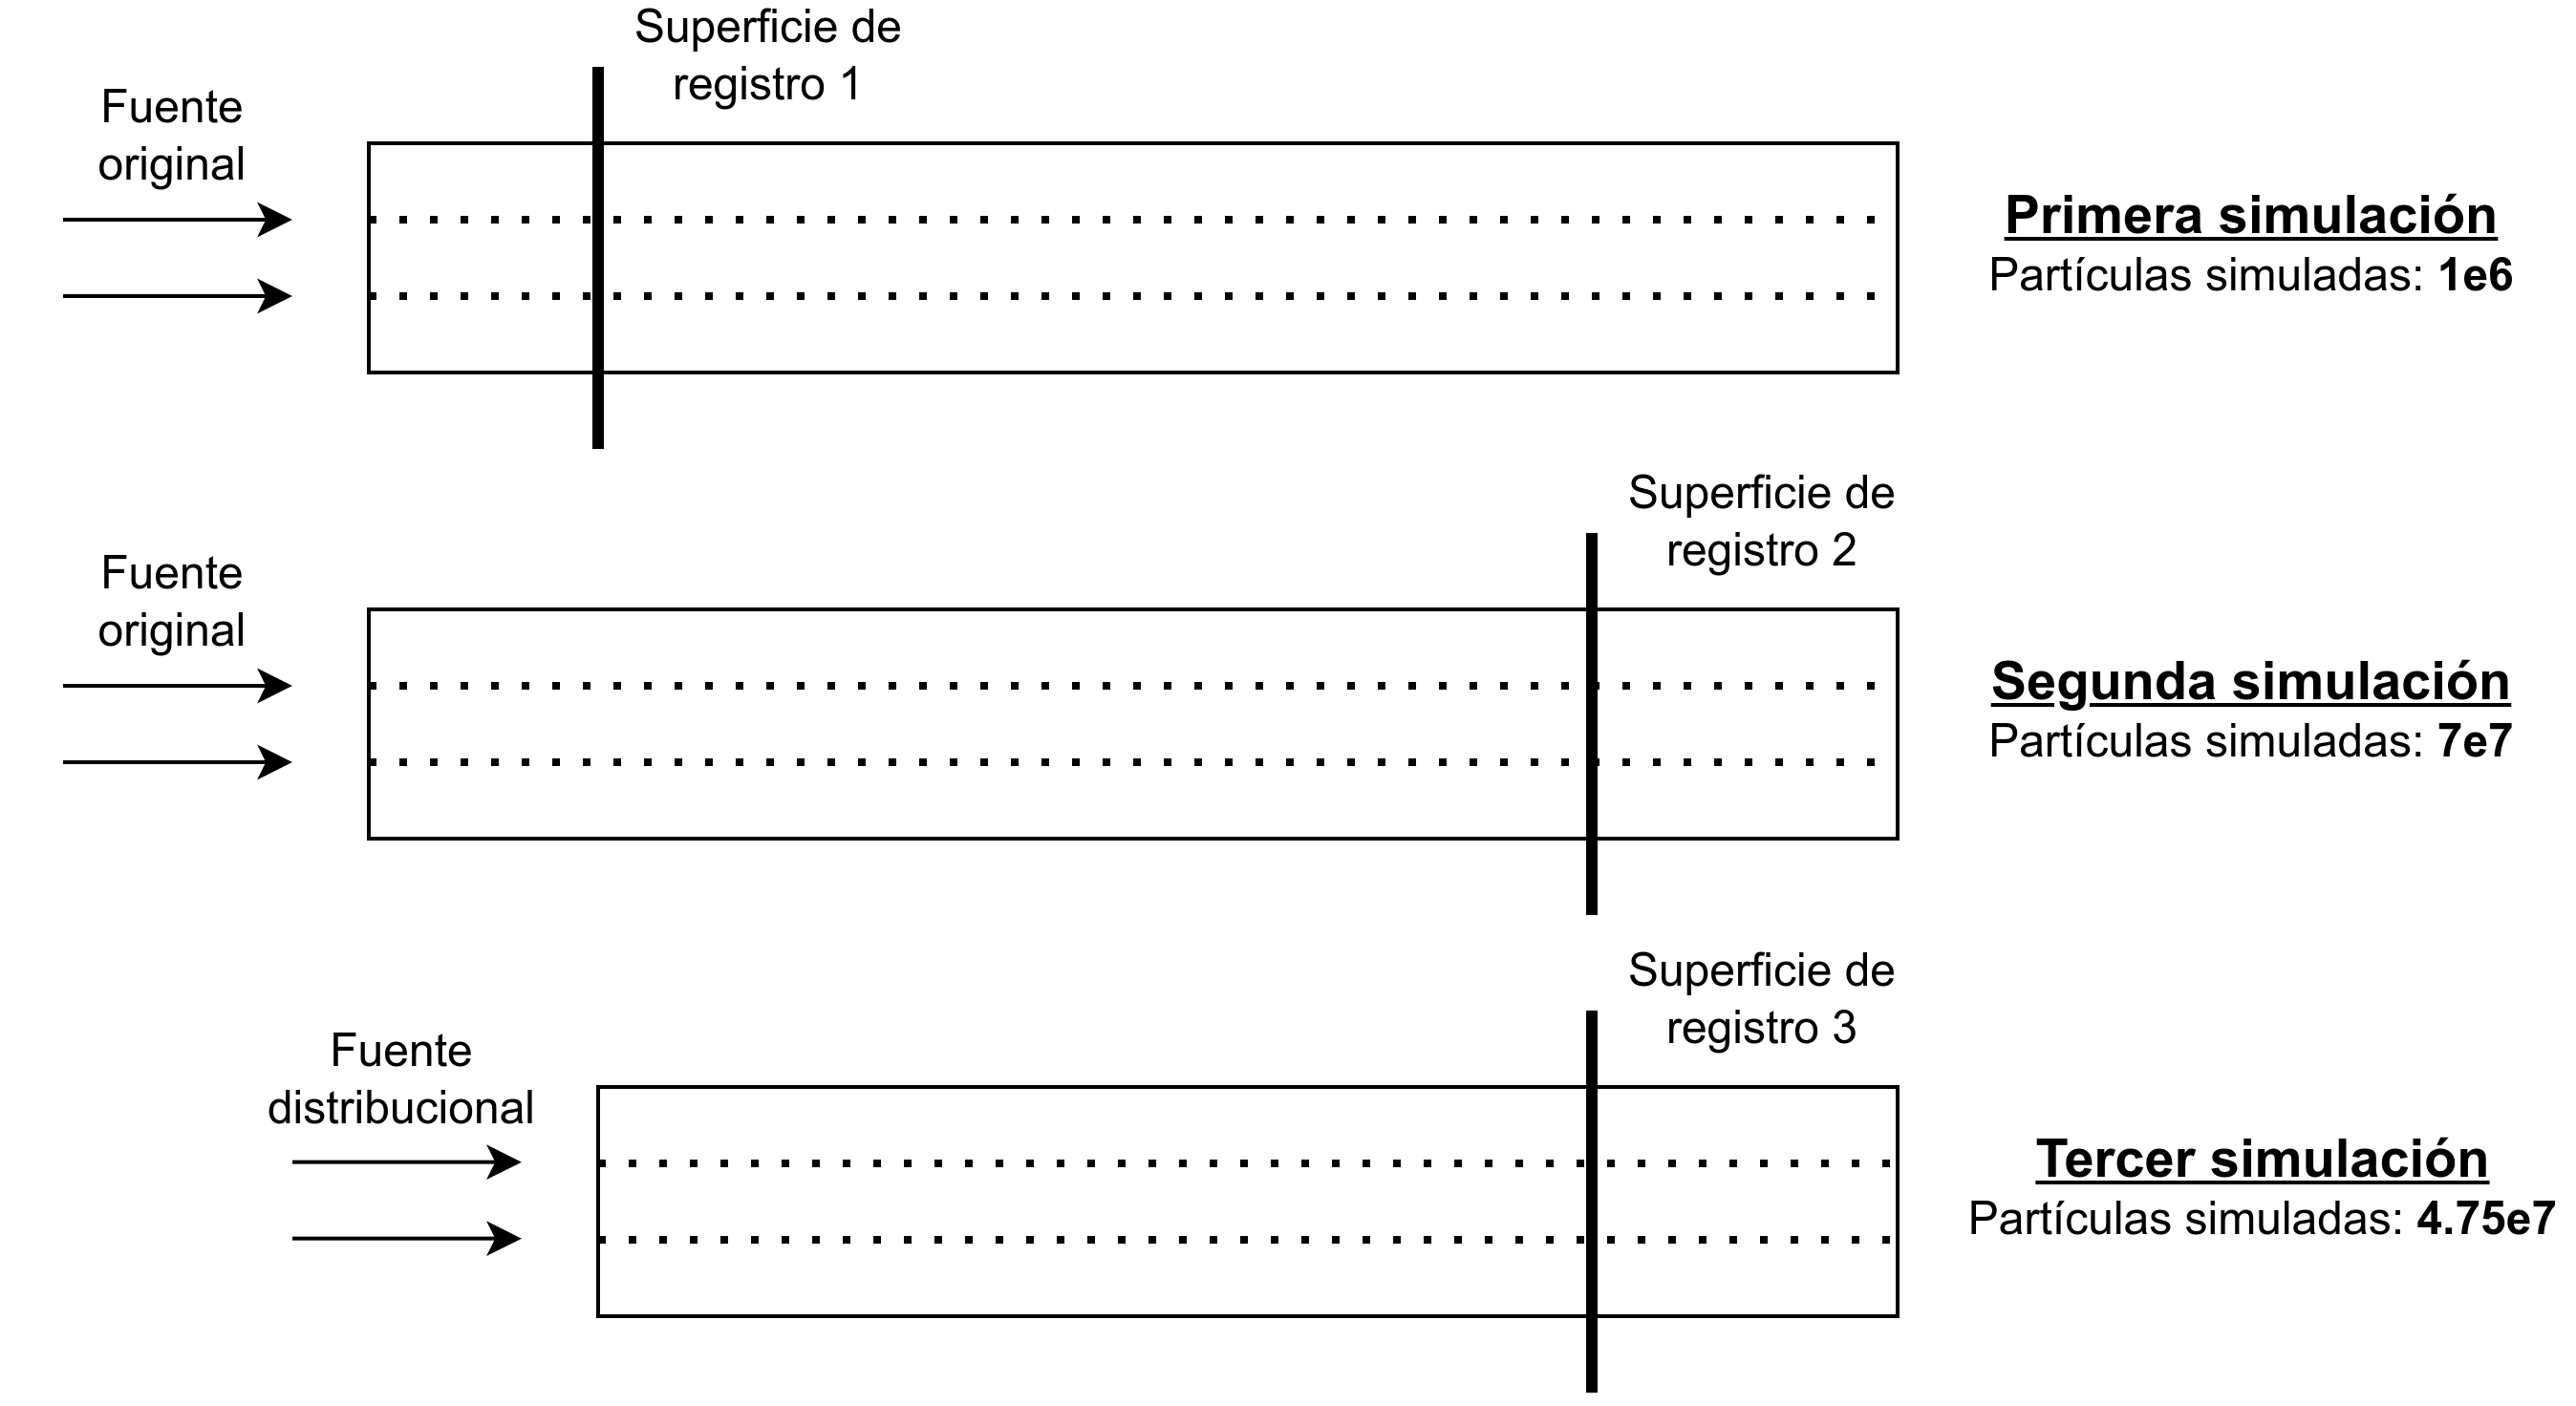
\includegraphics[width=\textwidth]{esquema_paralelepipedo.png}
    \caption{Esquema del proceso de remuestreo y validación del método implementado.}
    \label{fig:esquema_remuestreo}
\end{figure}

\section{Descripción del modelo simulado en \texttt{OpenMC}}

El modelo utilizado en las simulaciones consiste en un canal interno de vacío rodeado lateralmente por agua liviana. El sistema se diseñó como un paralelepípedo de agua con dimensiones $15\,\text{cm} \times 15\,\text{cm} \times 100\,\text{cm}$, que alberga en su interior un canal de vacío con sección transversal cuadrada de $3\,\text{cm} \times 3\,\text{cm}$, orientado en dirección del eje $z$. En la Figura \ref{fig:modelo_simulado_openmc} se presenta un esquema del modelo implementado en \texttt{OpenMC}.

\begin{figure}[h]
    \centering
    \includegraphics[width=\textwidth]{paralelepipedo_3.png}
    \caption{Esquema del modelo simulado en \texttt{OpenMC}.}
    \label{fig:modelo_simulado_openmc}
\end{figure}

La fuente de neutrones utilizada se definió sobre la cara de entrada del sistema (ubicada en $z = 0,\text{cm}$) y consistió en neutrones monoenergéticos con energía de $E = 1\,\text{MeV}$ y colimados en dirección del eje $z$ (con coseno direccional $\mu = \cos(\theta) = 1$). Esta configuración genera dos poblaciones de neutrones claramente diferenciadas: la primera, formada por neutrones que atraviesan el canal de vacío sin colisiones y mantienen tanto su energía inicial como su dirección; y la segunda, constituida por neutrones que interactúan con el moderador de agua, sufriendo dispersión angular y pérdida energética.

Para el análisis y posterior generación de la fuente, se registró un archivo de partículas sobre una superficie intermedia situada en $z = 15\,\text{cm}$. Este archivo contiene información sobre ambas poblaciones mencionadas, es decir, neutrones no colisionados y neutrones dispersados.

Durante las simulaciones se determinó el flujo escalar neutrónico a lo largo del canal, tanto dentro del canal de vacío como en el moderador circundante.

Para optimizar la estadística en regiones con baja presencia de partículas, particularmente en el agua, se implementó la técnica de ventanas de peso disponible en \texttt{OpenMC}. Este método actualiza los pesos de las partículas durante la simulación, permitiendo obtener mejorar estadística.

\section{Descripción del archivo de partículas original} 

El archivo de partículas fue registrado en una primera simulación del tubo de vacío desde el comienzo de la geometría. Corresponde a partículas registradas en una superficie ubicada a 15cm del inicio de la geometría. La lista contiene tanto neutrones que atraviesan la sección del canal, como neutrones que viajan por el agua. Sin embargo, la mayor proporción de peso estadístico se encuentra dentro del tubo de vacío, lo cual se corrobora tanto en la proyección $X$-$Y$, donde se observa una distribución más intensa contenida en un cuadrado correspondiente a la sección del tubo, como en la Tabla \ref{tab:particulas_pesos}, que presenta la cantidad de partículas y peso estadístico registrado por región. La Figura \ref{fig:trackfile1_x_y} muestra la proyección de los neutrones en el plano $X$-$Y$.

\begin{table}[H]
    \centering
    \begin{tabular}{lccccc}
        \toprule
        & & \multicolumn{2}{c}{Cantidad registrada [\#]} & \multicolumn{2}{c}{Densidad [\#/cm$^2$]} \\
        \cmidrule(lr){3-4} \cmidrule(lr){5-6}
        Región & Área [cm$^2$] & Partículas & Peso estad. & Partículas & Peso estad. \\
        \midrule
        Vacío & 9 & 62.523 & 46.862 & 6.947 & 5.207 \\
        Agua  & 216 & 390.412 & 44.938 & 1.807 & 208 \\
        \midrule
        Total & 225 & 452.935 & 91.800 & -- & -- \\
        \bottomrule
    \end{tabular}
    \caption{Resumen de partículas y peso estadístico registrados en la superficie intermedia ($z = 15$~cm) para cada región. Se informa también el área de cada región, así como la densidad de partículas y peso estadístico.}
    \label{tab:particulas_pesos}
\end{table}

\begin{figure}[H]
    \centering
    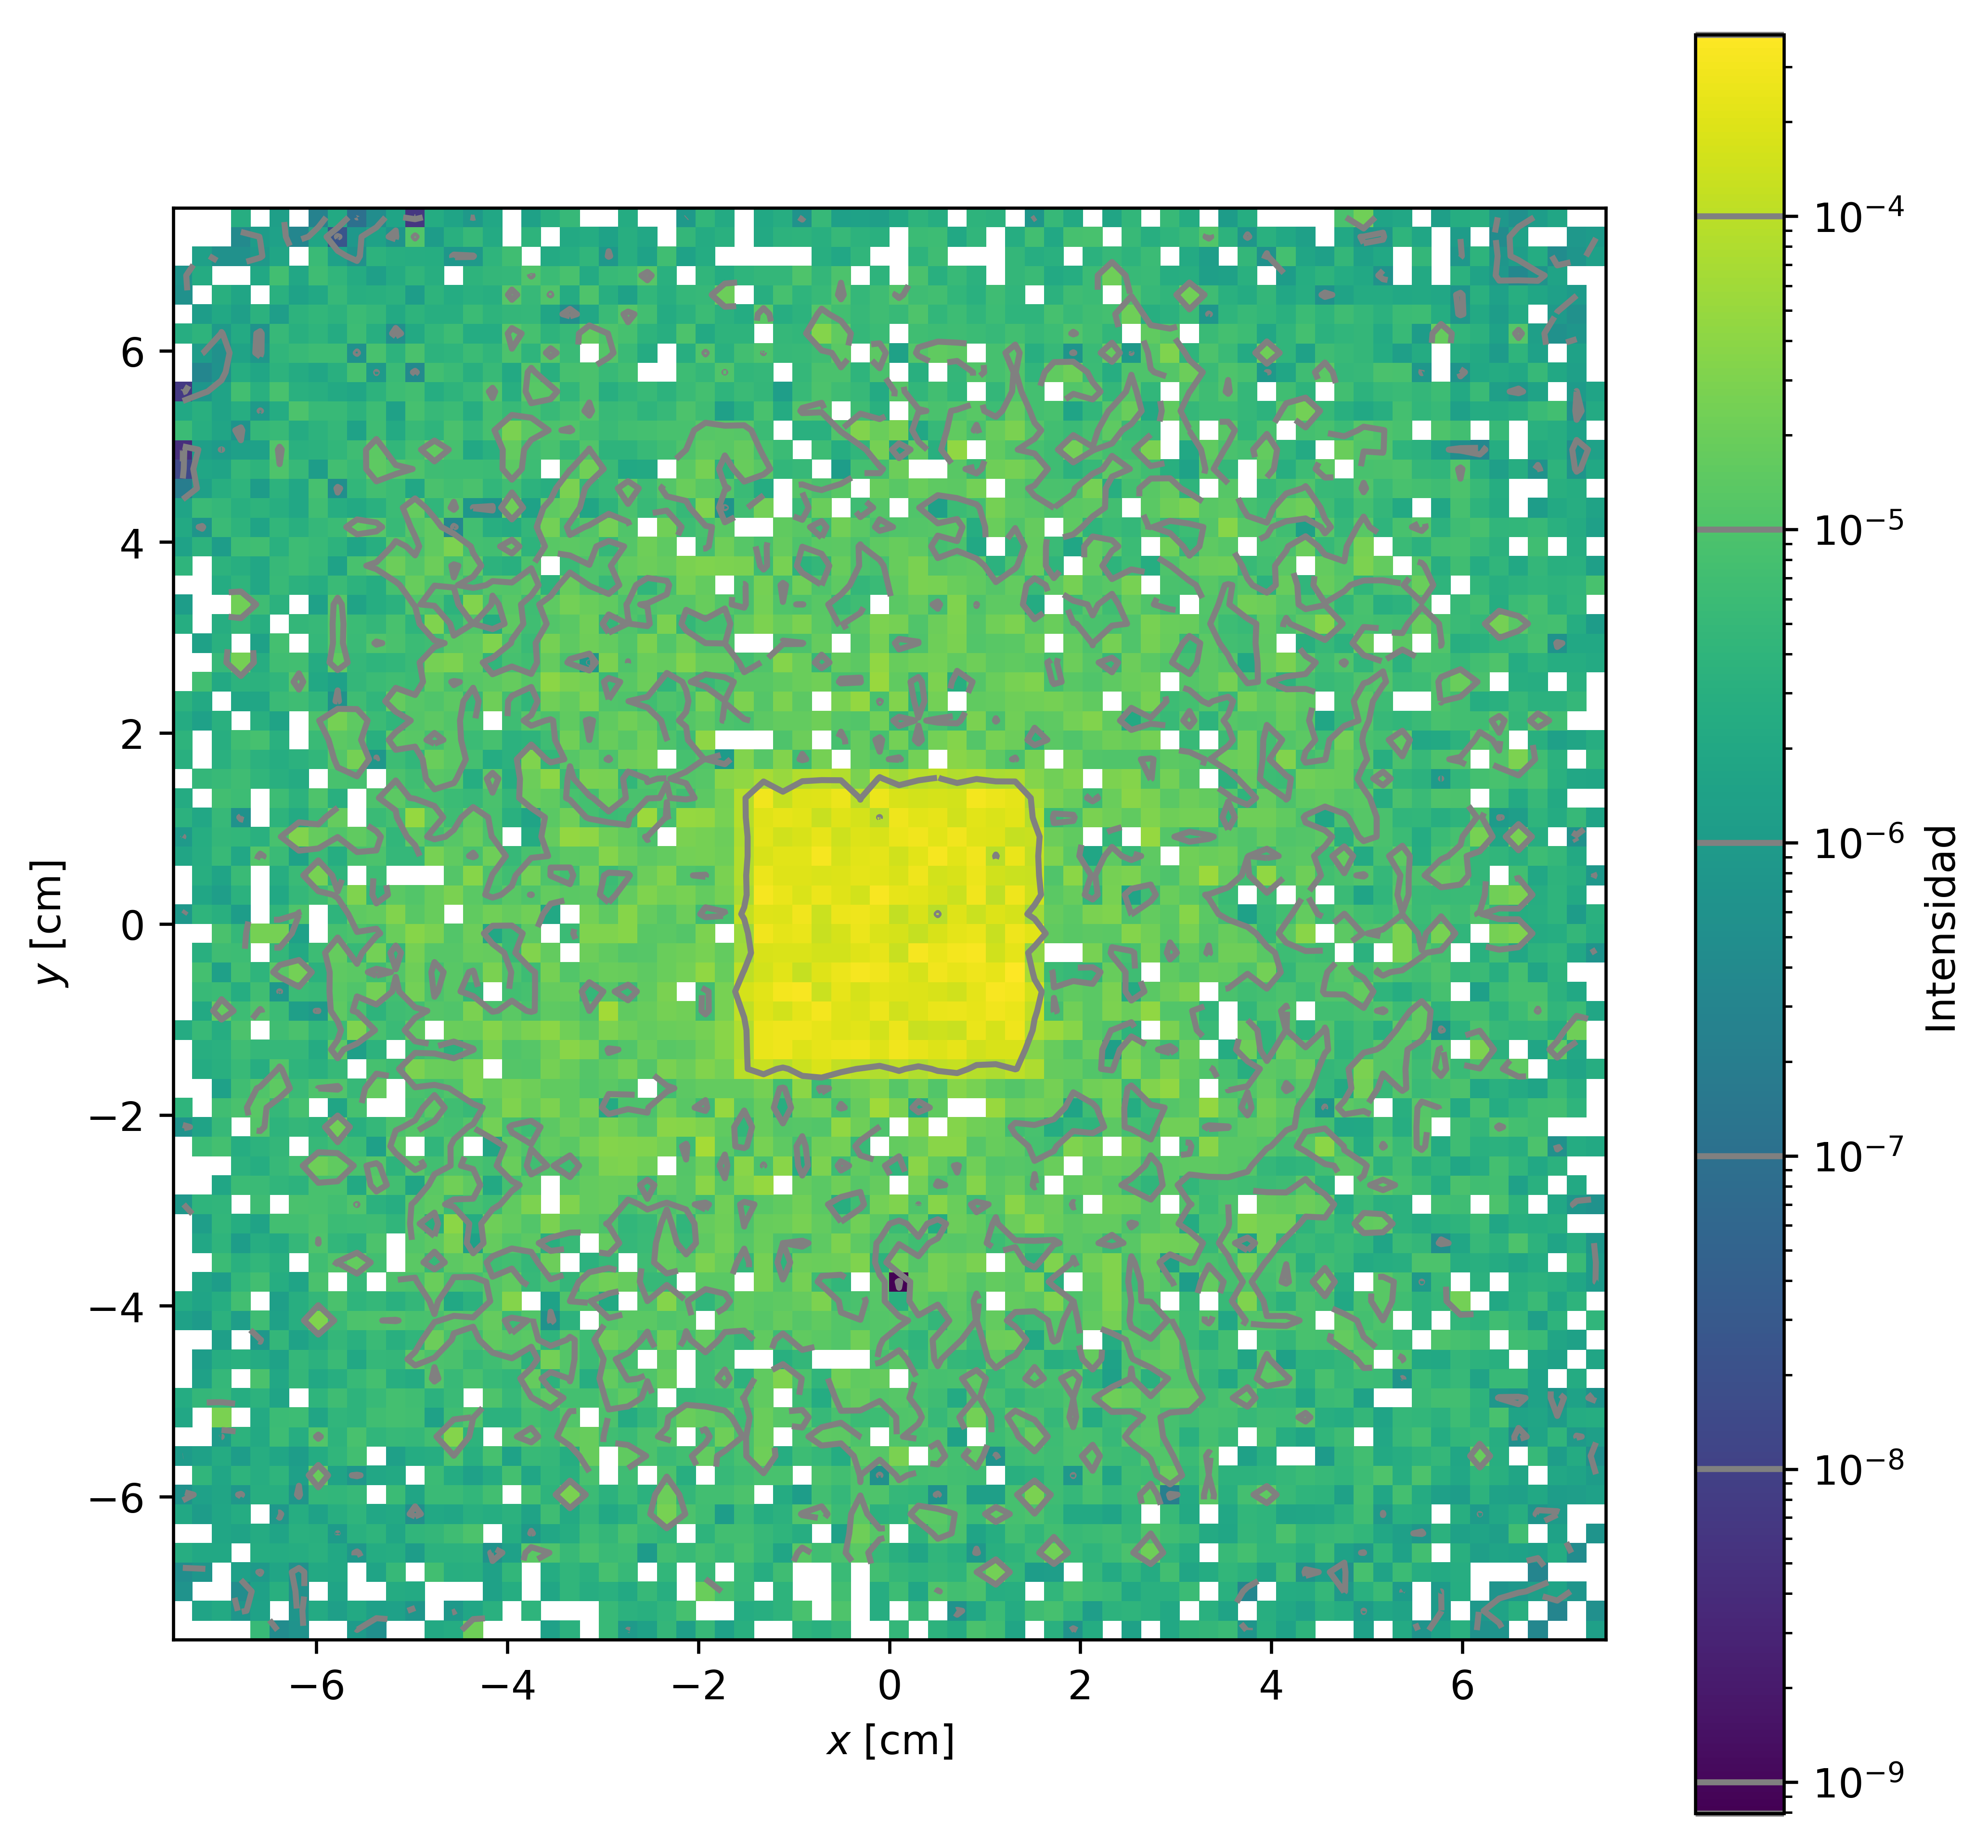
\includegraphics[width=0.75\textwidth]{figs/fig4_1.png}
    \caption{Distribución de $X$ vs $Y$ para el archivo de partículas registrado en la primera simulación del tubo de vacío.}
    \label{fig:trackfile1_x_y}
\end{figure}

Este conjunto contiene dos poblaciones de neutrones claramente diferenciadas. La primera corresponde a neutrones que no han sufrido colisiones: todos ellos presentan dirección $\mu = 1$ y una letargía fija correspondiente a una energía de $E = 1~MeV$, donde $\textit{letargía} = ln(E_0/E)$ con $E_0 = 20~MeV$. Estos valores coinciden con la configuración de la fuente original, la cual fue definida como perfectamente colimada y monoenergética. La segunda población está compuesta por neutrones que han interactuado con el medio: en este caso, las distribuciones de $\mu$ y letargía se extienden de forma continua, reflejando los efectos introducidos por las colisiones. Este comportamiento se observa en la Figura\ref{fig:trackfile1_letargia_mu}, donde se presentan las distribuciones de letargía y $\mu$ correspondientes al archivo de partículas registrado en la primera simulación del tubo de vacío.

Este conjunto contiene dos poblaciones de neutrones claramente diferenciadas. La primera corresponde a neutrones que no han sufrido colisiones: todos ellos poseen dirección $\mu = 1$ y una letargía fija, correspondiente a $E = 1~MeV$, sin dispersión alguna, lo cual concuerda con que la fuente original fue configurada con estos valores de forma determinista. La segunda población incluye neutrones que han colisionado: en este caso, las distribuciones de $\mu$ y letargía son más amplias y continuas, reflejando la dispersión introducida por las interacciones. Este comportamiento se observa en la Figura \ref{fig:trackfile1_letargia_mu}, donde se presentan las distribuciones de letargía y $\mu$ para el archivo de partículas registrado en la primera simulación del tubo de vacío. 

\begin{figure}[H]
    \centering
    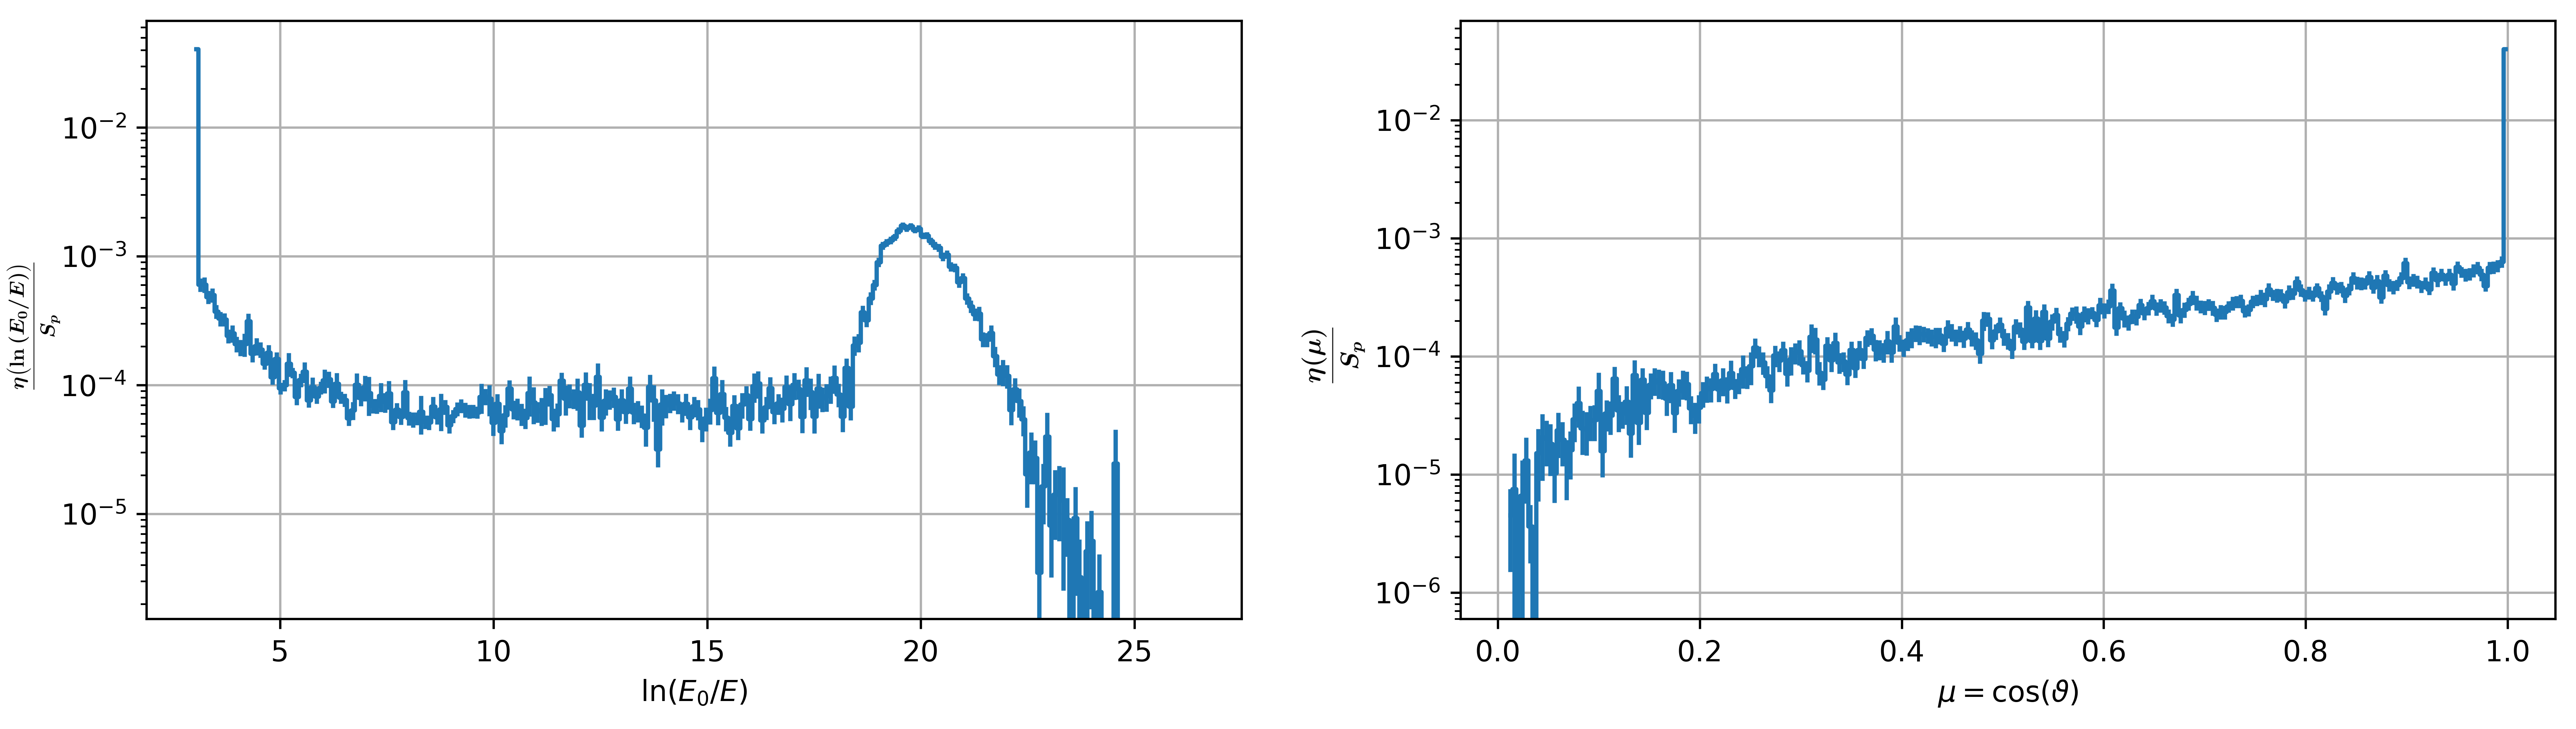
\includegraphics[width=\textwidth]{figs/fig4_2.png}
    \caption{Distribuciones de letargía y $\mu$ para el archivo de partículas registrado en la primera simulación del tubo de vacío, con escala logarítmica en el eje y. Se observa la presencia de dos poblaciones: una concentrada en $\mu = 1$ y letargía fija correspondiente a una energía de $E = 1~MeV$, montada sobre una distribución continua de neutrones colisionados.}
    \label{fig:trackfile1_letargia_mu}
\end{figure}

Esta doble estructura se evidencia particularmente en los gráficos bidimensionales de letargía vs. $\mu$, donde ambas poblaciones aparecen como conjuntos diferenciados. Tal como se muestra en la Figura \ref{fig:trackfile1_letargia_mu_2}, los neutrones no colisionados se concentran en un único punto en $\mu = 1$ y letargía fija correspondiente a una energía de $E = 1~MeV$, mientras que los neutrones colisionados forman una distribución extendida continua, con un agrupamiento en la región de termalización. Este fenómeno plantea un desafío para los métodos de muestreo, al requerir una representación precisa tanto de distribuciones tipo delta como de distribuciones extendidas.


Tanto en la Figura~\ref{fig:trackfile1_x_y} como en la Figura~\ref{fig:trackfile1_letargia_mu_2} puede observarse que existen regiones del espacio de fases donde no se registran neutrones. Esto se debe a que el archivo de partículas original contiene una cantidad finita de neutrones, lo que limita la cobertura en determinadas regiones del espacio de fases. El objetivo del método propuesto consiste en remuestrear dicho archivo original para generar un nuevo conjunto de partículas que preserve las correlaciones presentes, pero que a su vez mejore la estadística en aquellas regiones originalmente poco representadas.


\begin{figure}[H]
    \centering
    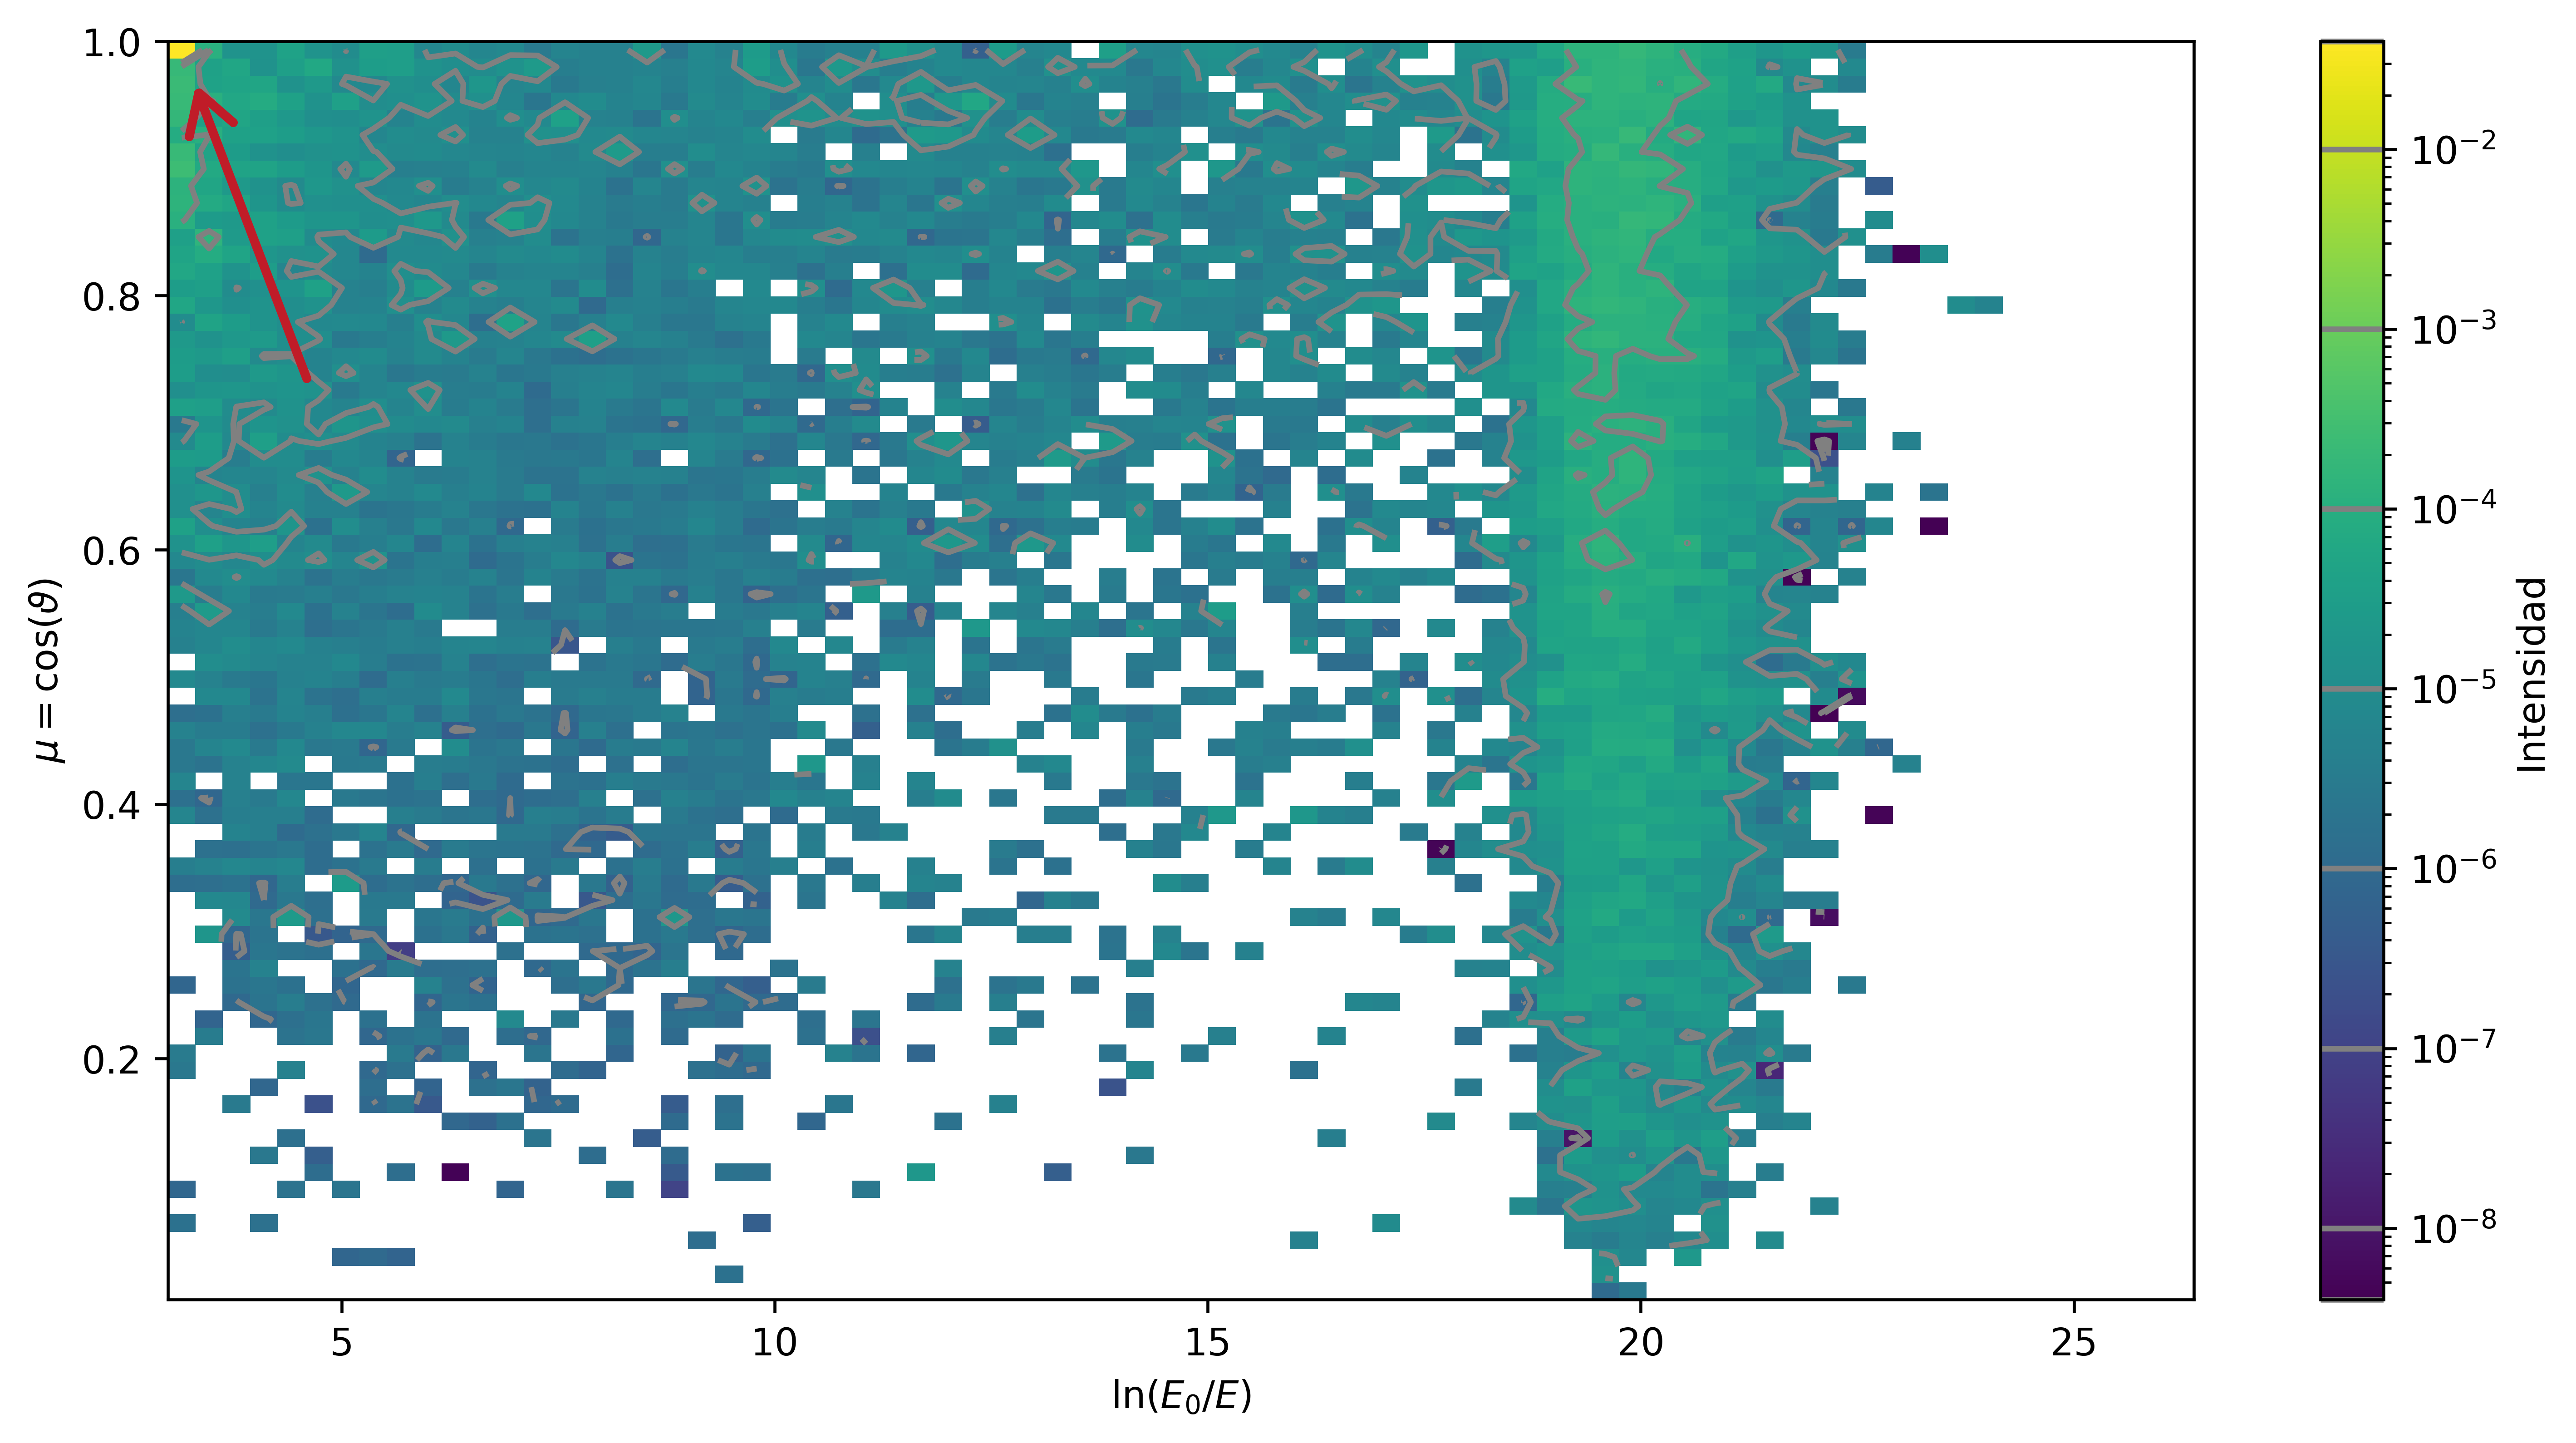
\includegraphics[width=0.9\textwidth]{figs/fig4_3.png}
    \caption{Distribuciones de letargía vs $\mu$ para el archivo de partículas original. Se observa la presencia de un conjunto de neutrones graficados como un píxel en $\mu = 1$ y letargía mínima. A su vez se observa la presencia de un segundo conjunto de neutrones colisionados, que se distribuyen en el plano de forma continua, con un agrupamiento sobre letargía = 20, indicando la termalización de los neutrones.}
    \label{fig:trackfile1_letargia_mu_2}
\end{figure}

\section{Procesamiento preliminar del archivo de partículas}
\subsection{Metodología del análisis}
\label{sec:metodologia-analisis}

El análisis realizado en este capítulo se centra en evaluar la influencia del tipo de bineado aplicado, así como la incorporación de bordes manuales en la segmentación del espacio de fases. Los tipos de bineado considerados son:
\begin{itemize}
    \item Caso 1: bineado uniforme sin bordes manuales.
    \item Caso 2: bineado uniforme con bordes definidos por el usuario.
    \item Caso 3: bineado adaptativo sin bordes manuales.
    \item Caso 4: bineado adaptativo con bordes definidos por el usuario.
\end{itemize}

Los bordes manuales son establecidos debido al conocimiento previo de la fuente utilizada para diferenciar poblaciones de neutrones. Concretamente, se incorporan bordes en la variable letargía y en la dirección cosenoidal ($\mu$) para distinguir los neutrones que no han colisionado. Adicionalmente, se incluyen bordes espaciales en las coordenadas $X$ e $Y$ para separar los neutrones que atraviesan el tubo de vacío respecto de aquellos que interactúan con el agua circundante.

Con el objetivo de realizar un análisis consistente y evitar sesgos derivados del procedimiento, se mantiene constante en todos los casos el orden de procesamiento de las variables y la configuración de los histogramas. Esta etapa preliminar permite una comparación entre los cuatro métodos de bineado evaluados en esta sección. El orden seleccionado para el procesamiento es \texttt{[letargía, X, Y, $\mu$, $\phi$]}. Esta elección responde a que al inicio del procesamiento, la discretización se aplica sobre el conjunto completo de partículas, mientras que las variables procesadas posteriormente actúan sobre subconjuntos cada vez más reducidos. Por este motivo, se eligió comenzar con la letargía para priorizar describir el comportamiento espectral. A continuación se aplican las variables espaciales (\texttt{X} e \texttt{Y}), con el fin de preservar correctamente la ubicación de las partículas en regiones geométricamente diferenciadas (vacío o agua). Finalmente, se dejó para el último lugar la variable \texttt{$\phi$}, cuya distribución se espera relativamente uniforme, por lo que no requiere un nivel de detalle elevado.

Asimismo, se conservan fijos los números de bines utilizados en los histogramas macro y micro: se emplean \texttt{[5, 5, 5, 5]} bines para los macrogrupos y \texttt{[36, 36, 36, 36, 36]} para los microgrupos, respectivamente. Esta configuración constante garantiza que las comparaciones entre métodos se basen únicamente en el esquema de discretizacion utilizado y no en diferencias en la resolución.

Posteriormente, el análisis se estructura en tres partes:

\begin{itemize}
\item \textbf{Distribuciones de letargía:} se presentan y comparan las distribuciones de letargía obtenidas para cada uno de los cuatro esquemas evaluados, comparándolas contra la distribución registrada en el archivo original.
\item \textbf{Distribuciones de $\mu$:} se analizan de forma análoga las distribuciones de la variable direccional $\mu = \cos\theta$, evaluando en qué medida se preserva la estructura angular del haz en cada uno de los casos.

\item \textbf{Distribuciones espaciales $X$–$Y$:} se analizan los resultados mediante mapas bidimensionales para cada una de las configuraciones, comparando las distribuciones generadas contra las distribuciones originales.
\end{itemize}

\subsection{Distribuciones de letargía}
A continuación se analizan las distribuciones remuestreadas de letargía obtenidas mediante los 4 casos de configuración analizados.

En la Figura \ref{fig:let_1}, correspondiente al caso 1 de bineado uniforme sin bordes, se observa que esta configuración presenta limitaciones en regiones de alta densidad estadística. En particular, la delta en la zona de letargía correspondiente a una energía de $E = 1~MeV$ —asociada a neutrones no colisionados— es reemplazada por un escalón con el ancho del bin, perdiéndose el comportamiento tipo delta. Asimismo, en la región de termalización, la resolución es insuficiente para capturar adecuadamente los cambios de forma.

\begin{figure}[H]
    \centering
    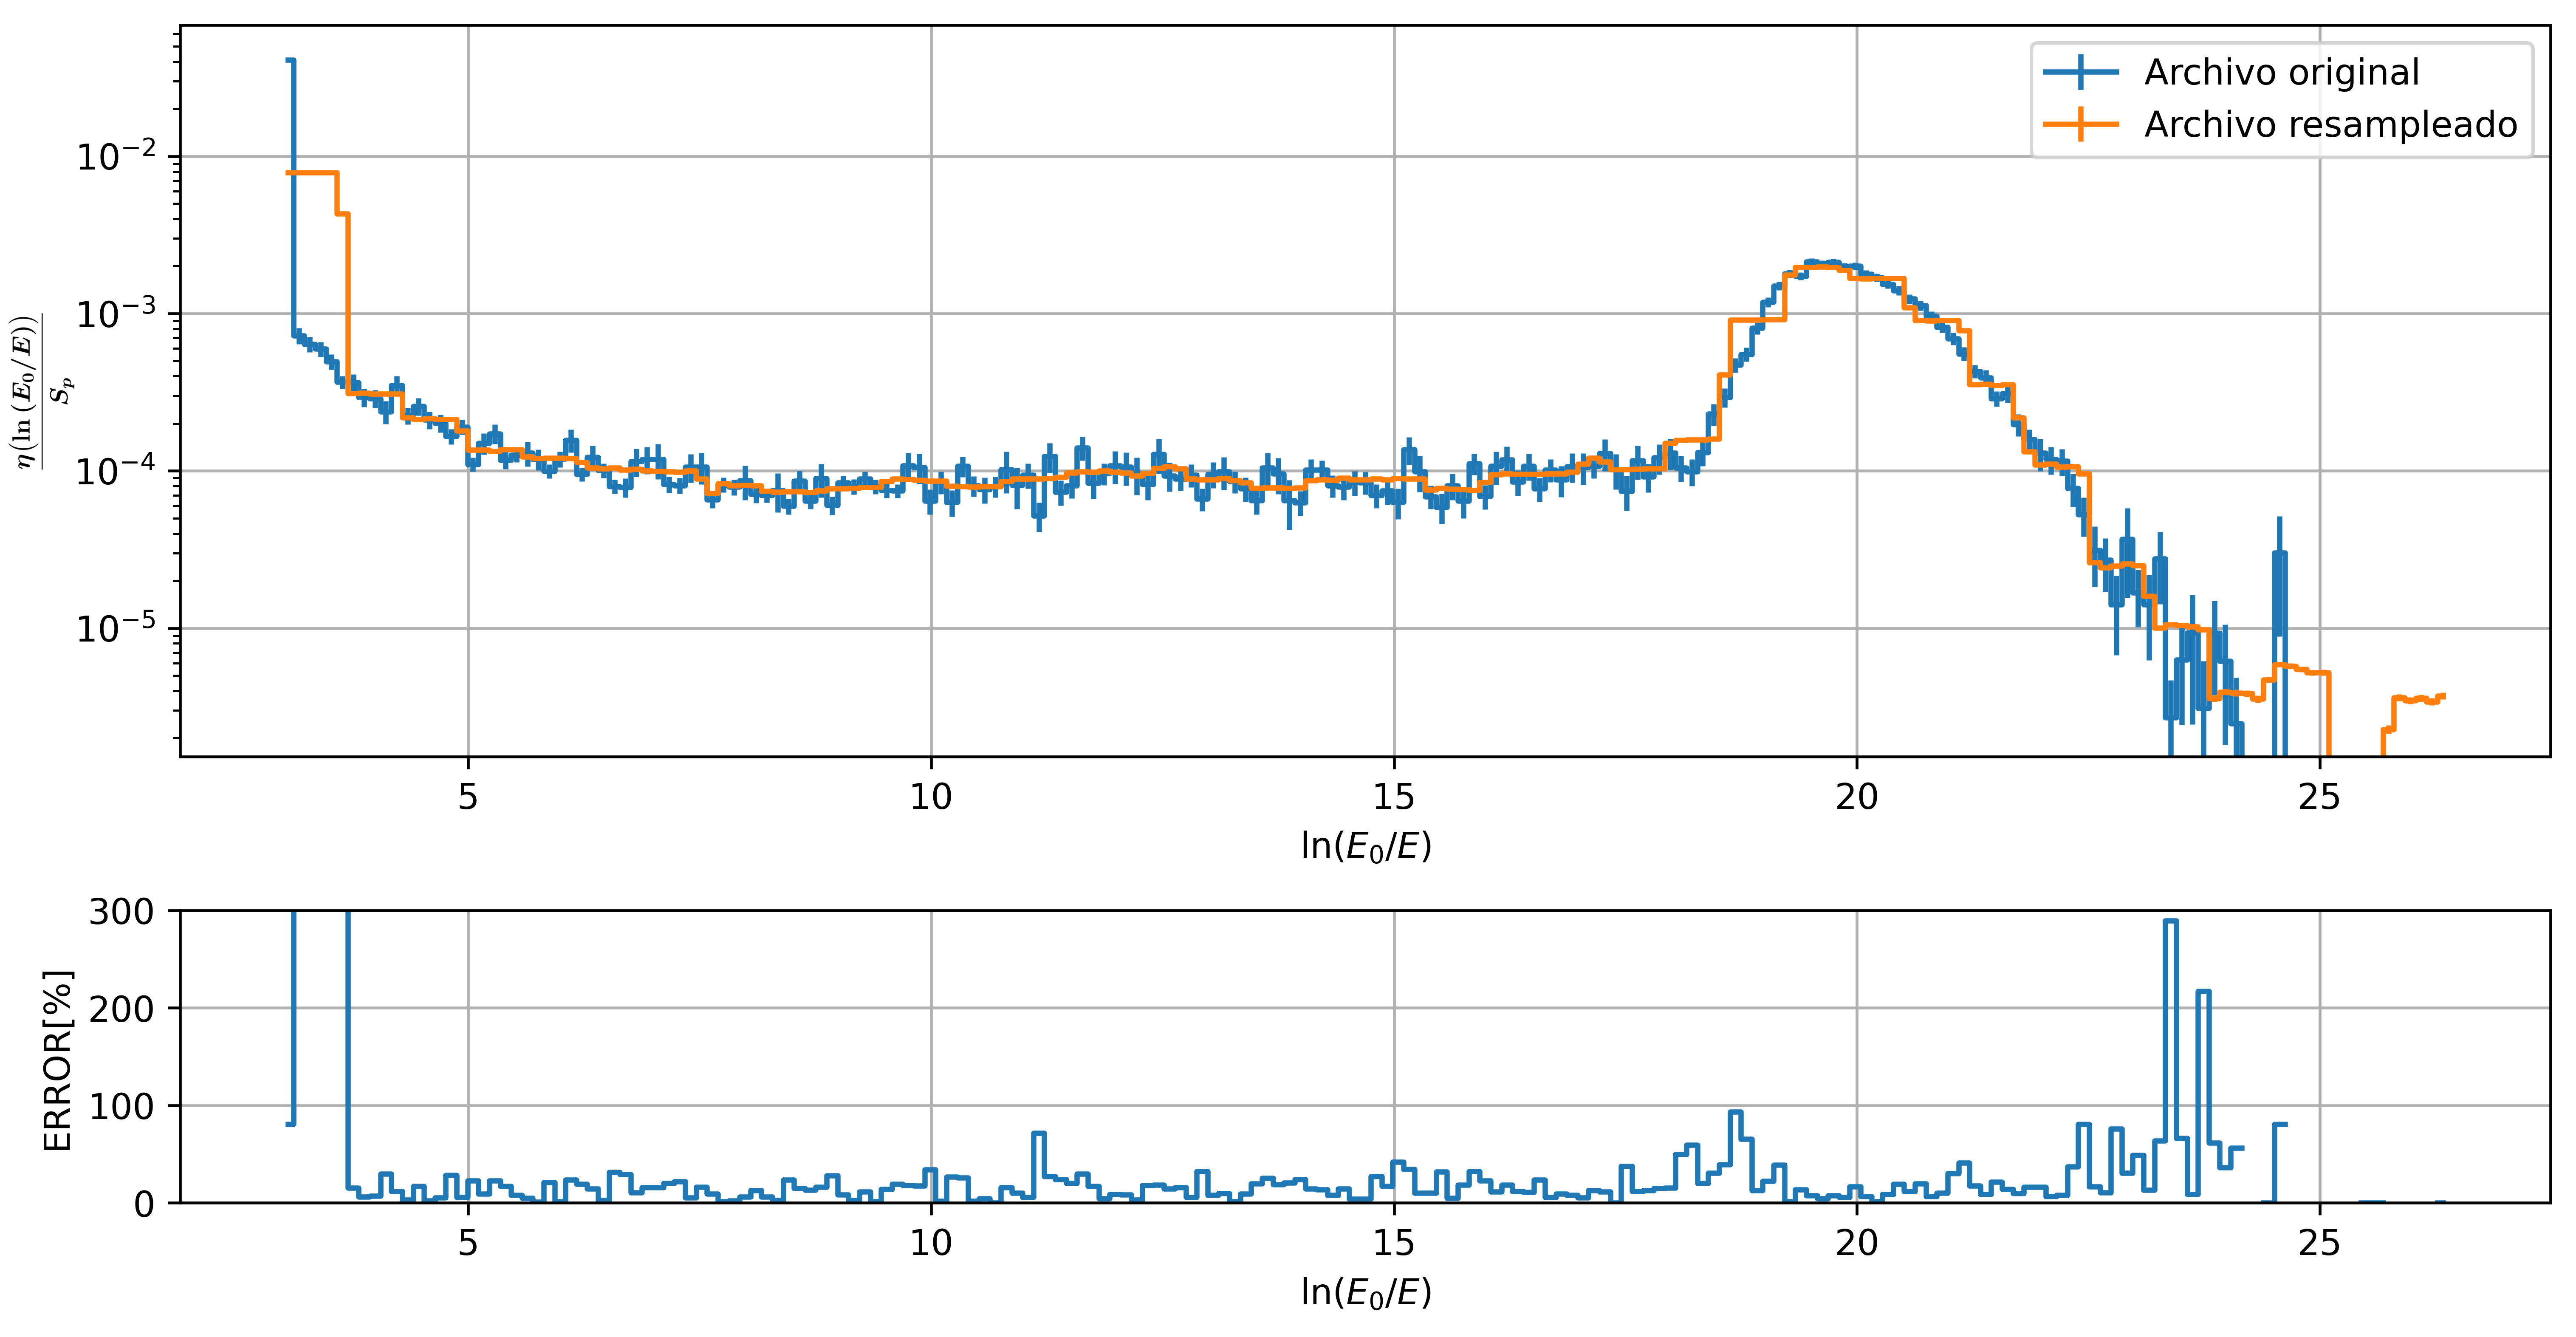
\includegraphics[width=\textwidth]{let_1.png}
    \caption{Distribución remuestreada de letargía para el caso de bineado uniforme sin bordes manuales.}
    \label{fig:let_1}
\end{figure}

La Figura \ref{fig:let_2} muestra el caso 2 en el que se introduce un borde manual para separar la letargía correspondiente a una energía de $E = 1~MeV$. Esta intervención permite mejorar la representación de la delta, capturando con mayor fidelidad los neutrones no colisionados. Sin embargo, el resto de la distribución sigue estando limitada por la resolución uniforme, en particular en la zona de termalización.

En la Figura \ref{fig:let_3}, se presenta el resultado del caso 3 utilizando histogramas adaptativos sin bordes manuales. Este método asigna una mayor densidad de bines en zonas con mayor estadística, lo que permite una mejor representación tanto de la delta en letargía correspondiente a una energía de $E = 1~MeV$ como de la región de termalización. Se observa un seguimiento más suave y detallado de la distribución, y una reducción del error relativo en las zonas relevantes.

\begin{figure}[H]
    \centering
    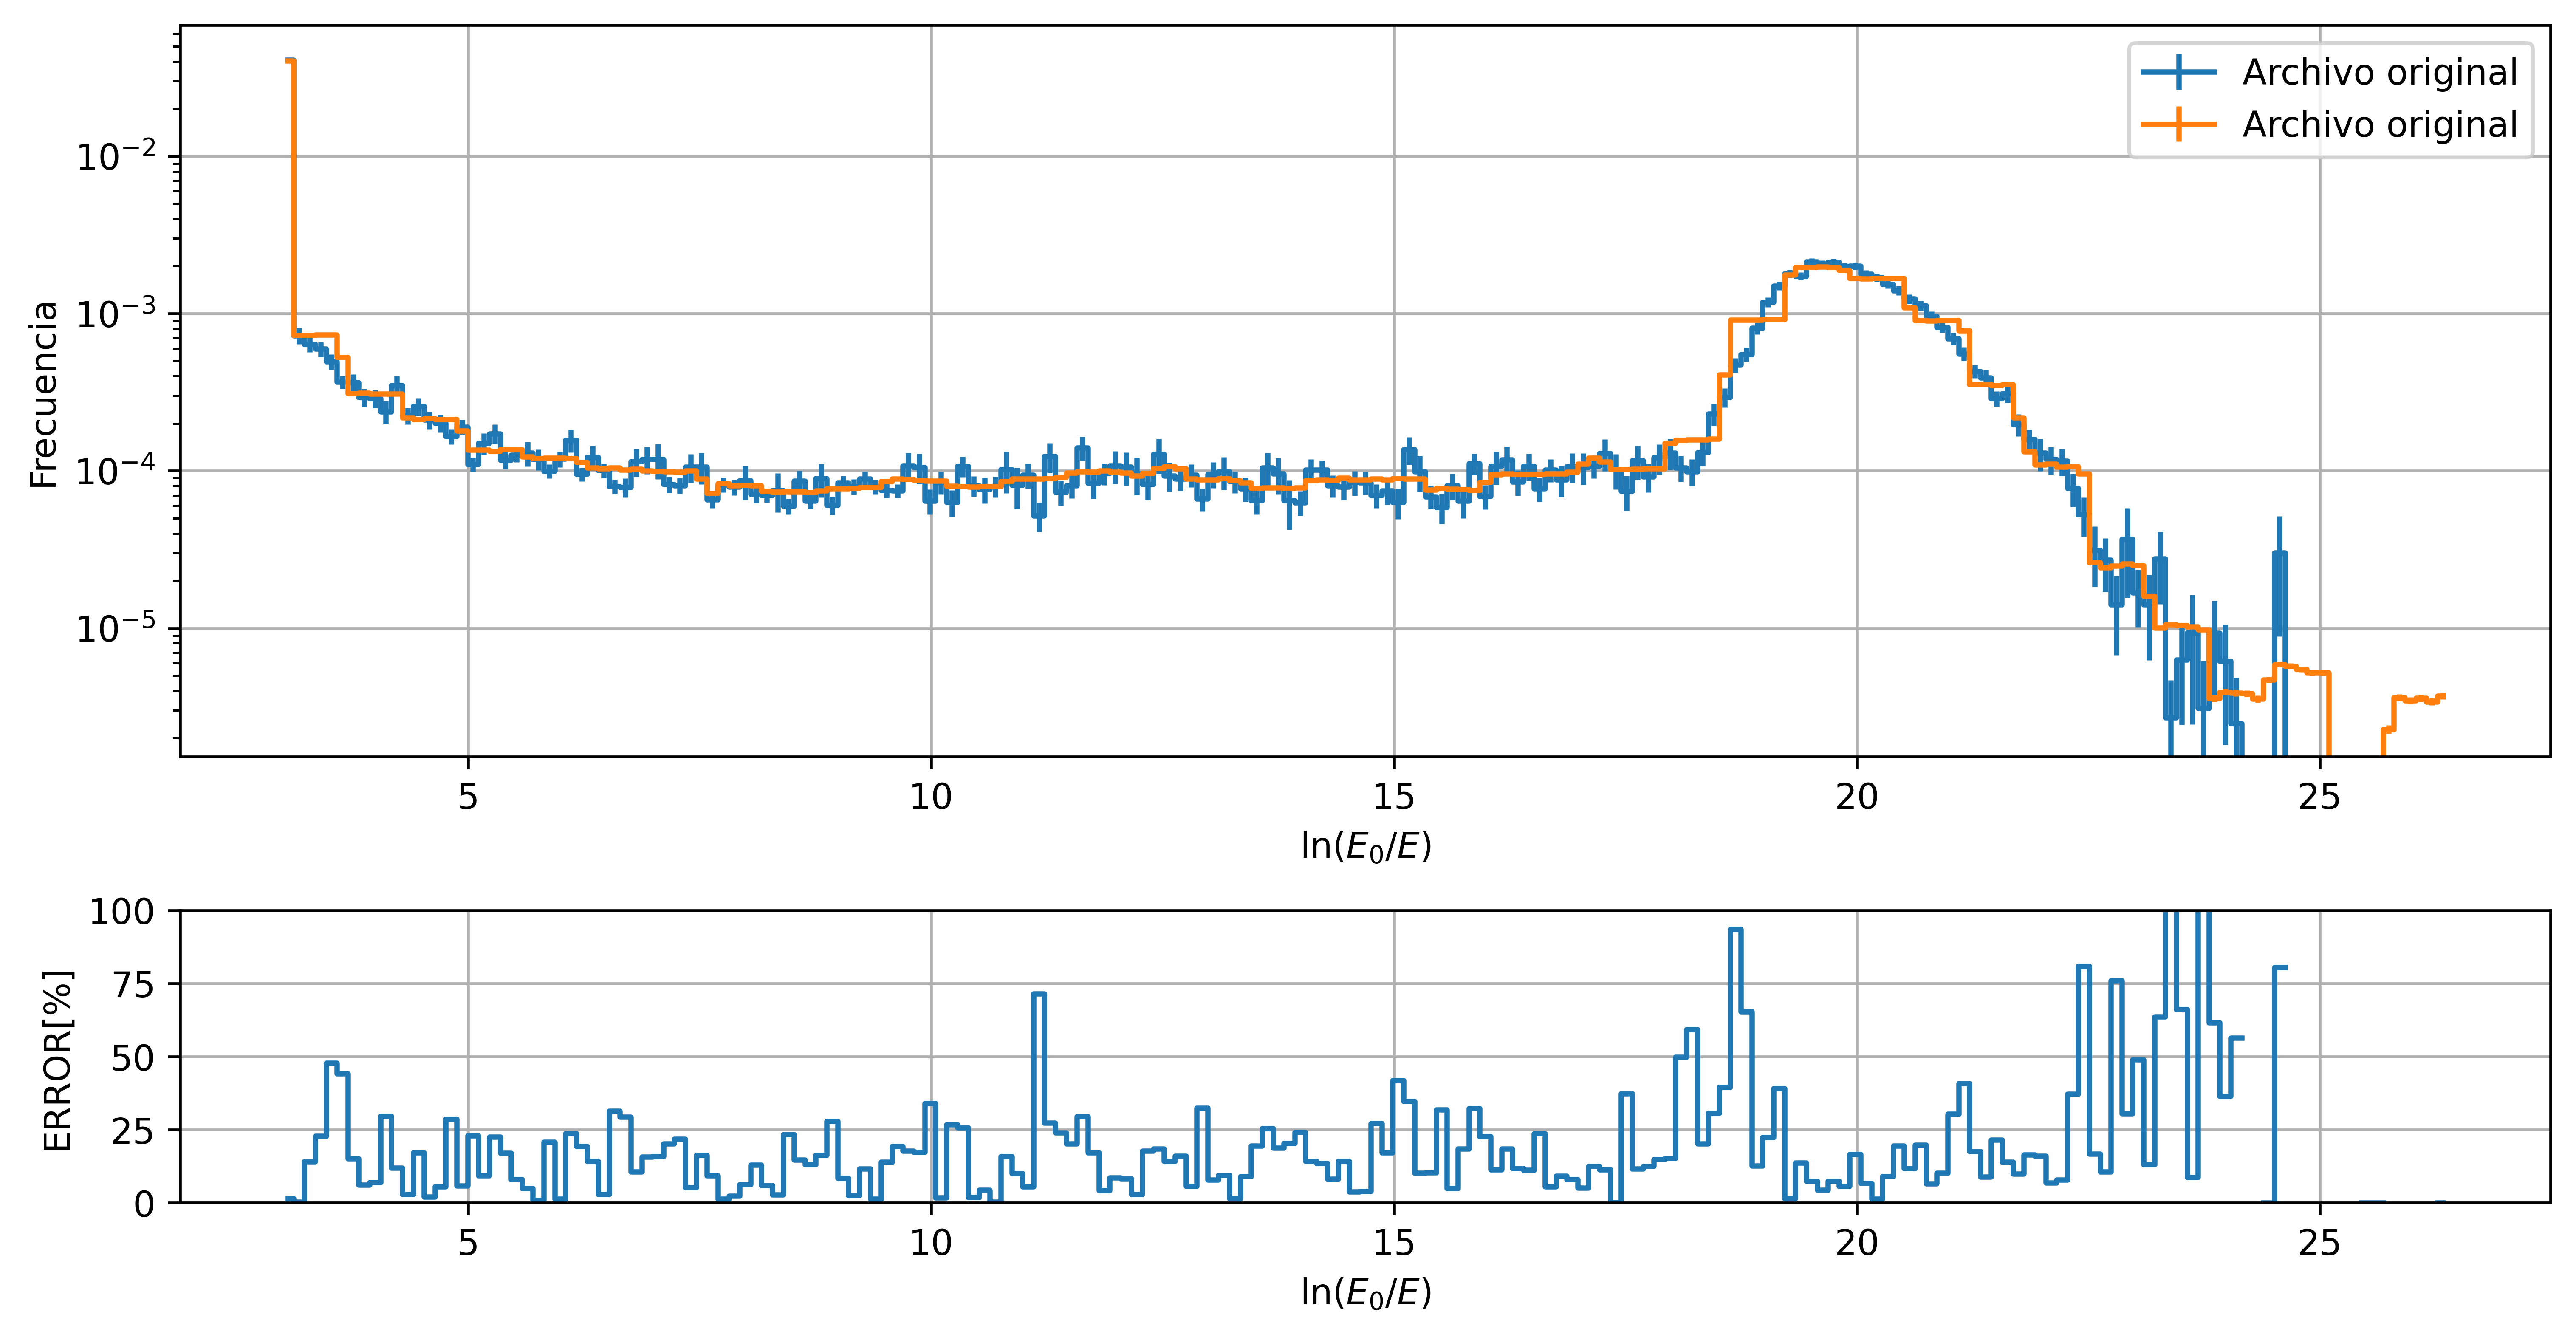
\includegraphics[width=\textwidth]{let_2.png}
    \caption{Distribución remuestreada de letargía para el caso de bineado uniforme con borde manual en la zona de letargía correspondiente a una energía de $E = 1~MeV$.}
    \label{fig:let_2}
\end{figure}

Finalmente, en la Figura \ref{fig:let_4}, se muestra el resultado del caso 4 con el método adaptativo con bordes manuales. No se observan diferencias significativas con respecto al caso sin bordes, lo que demuestra que el algoritmo es capaz de identificar y segmentar eficientemente las zonas relevantes de forma autónoma, incluso sin información previa de la fuente brindada por el borde manual.

\begin{figure}[H]
    \centering
    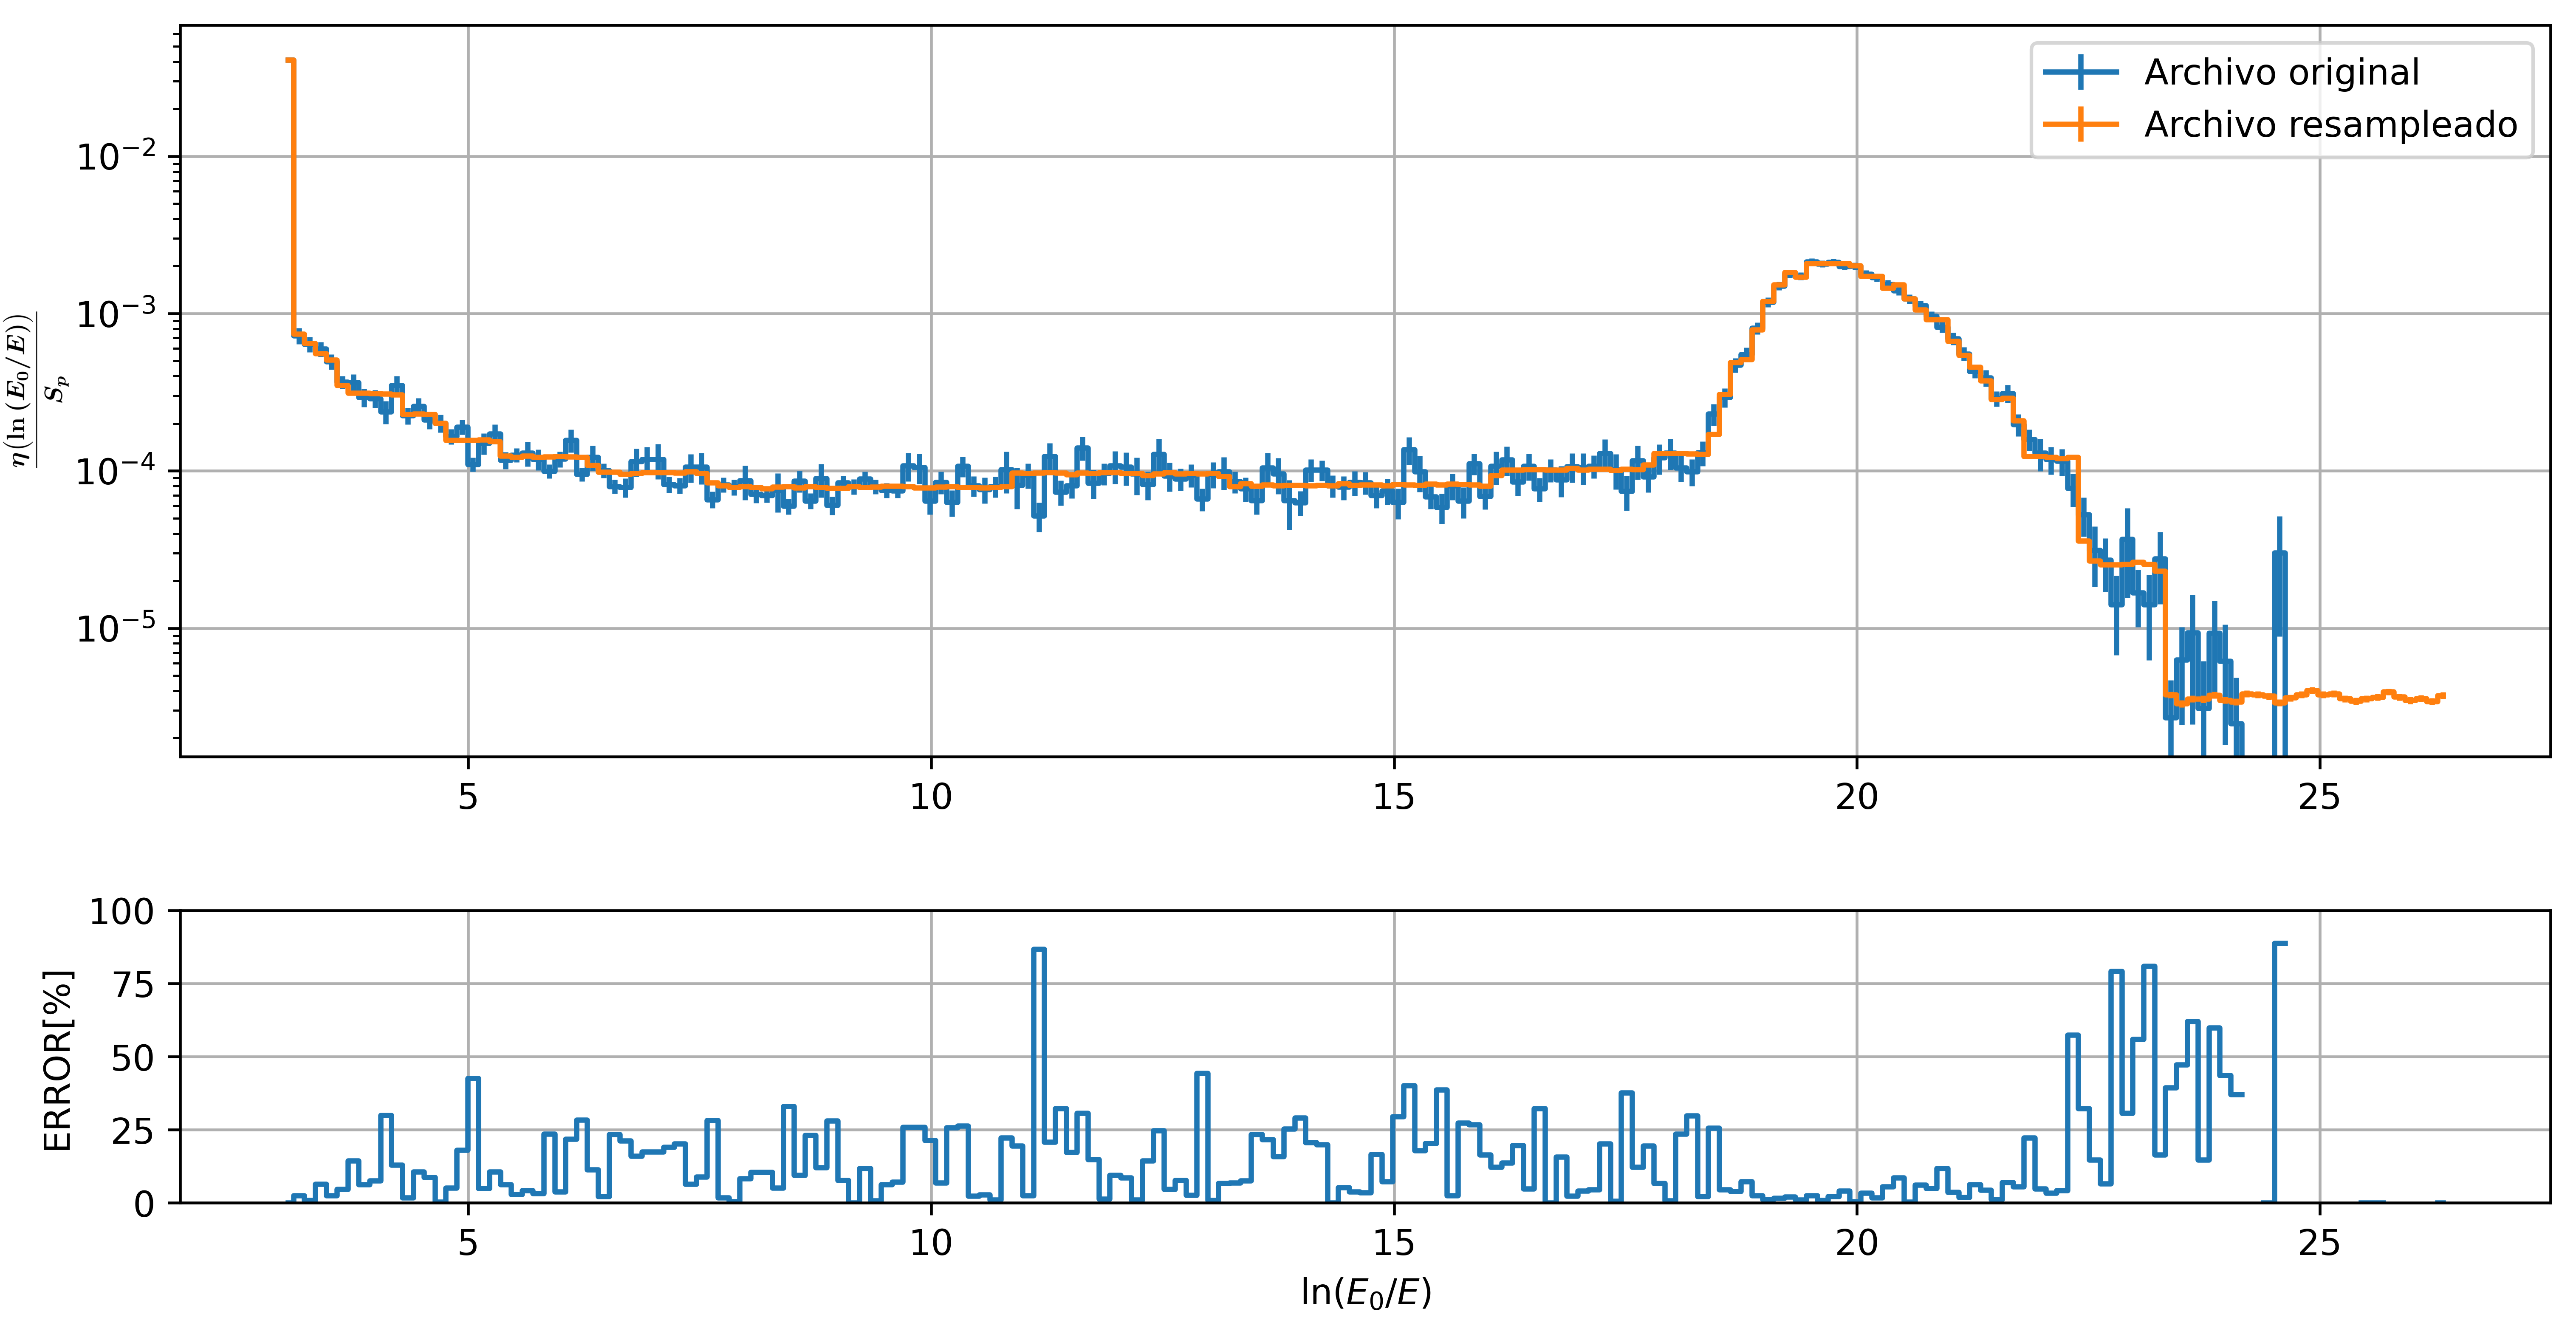
\includegraphics[width=\textwidth]{let_3.png}
    \caption{Distribución remuestreada de letargía para el caso de bineado adaptativo sin bordes manuales.}
    \label{fig:let_3}
\end{figure}

\begin{figure}[H]
    \centering
    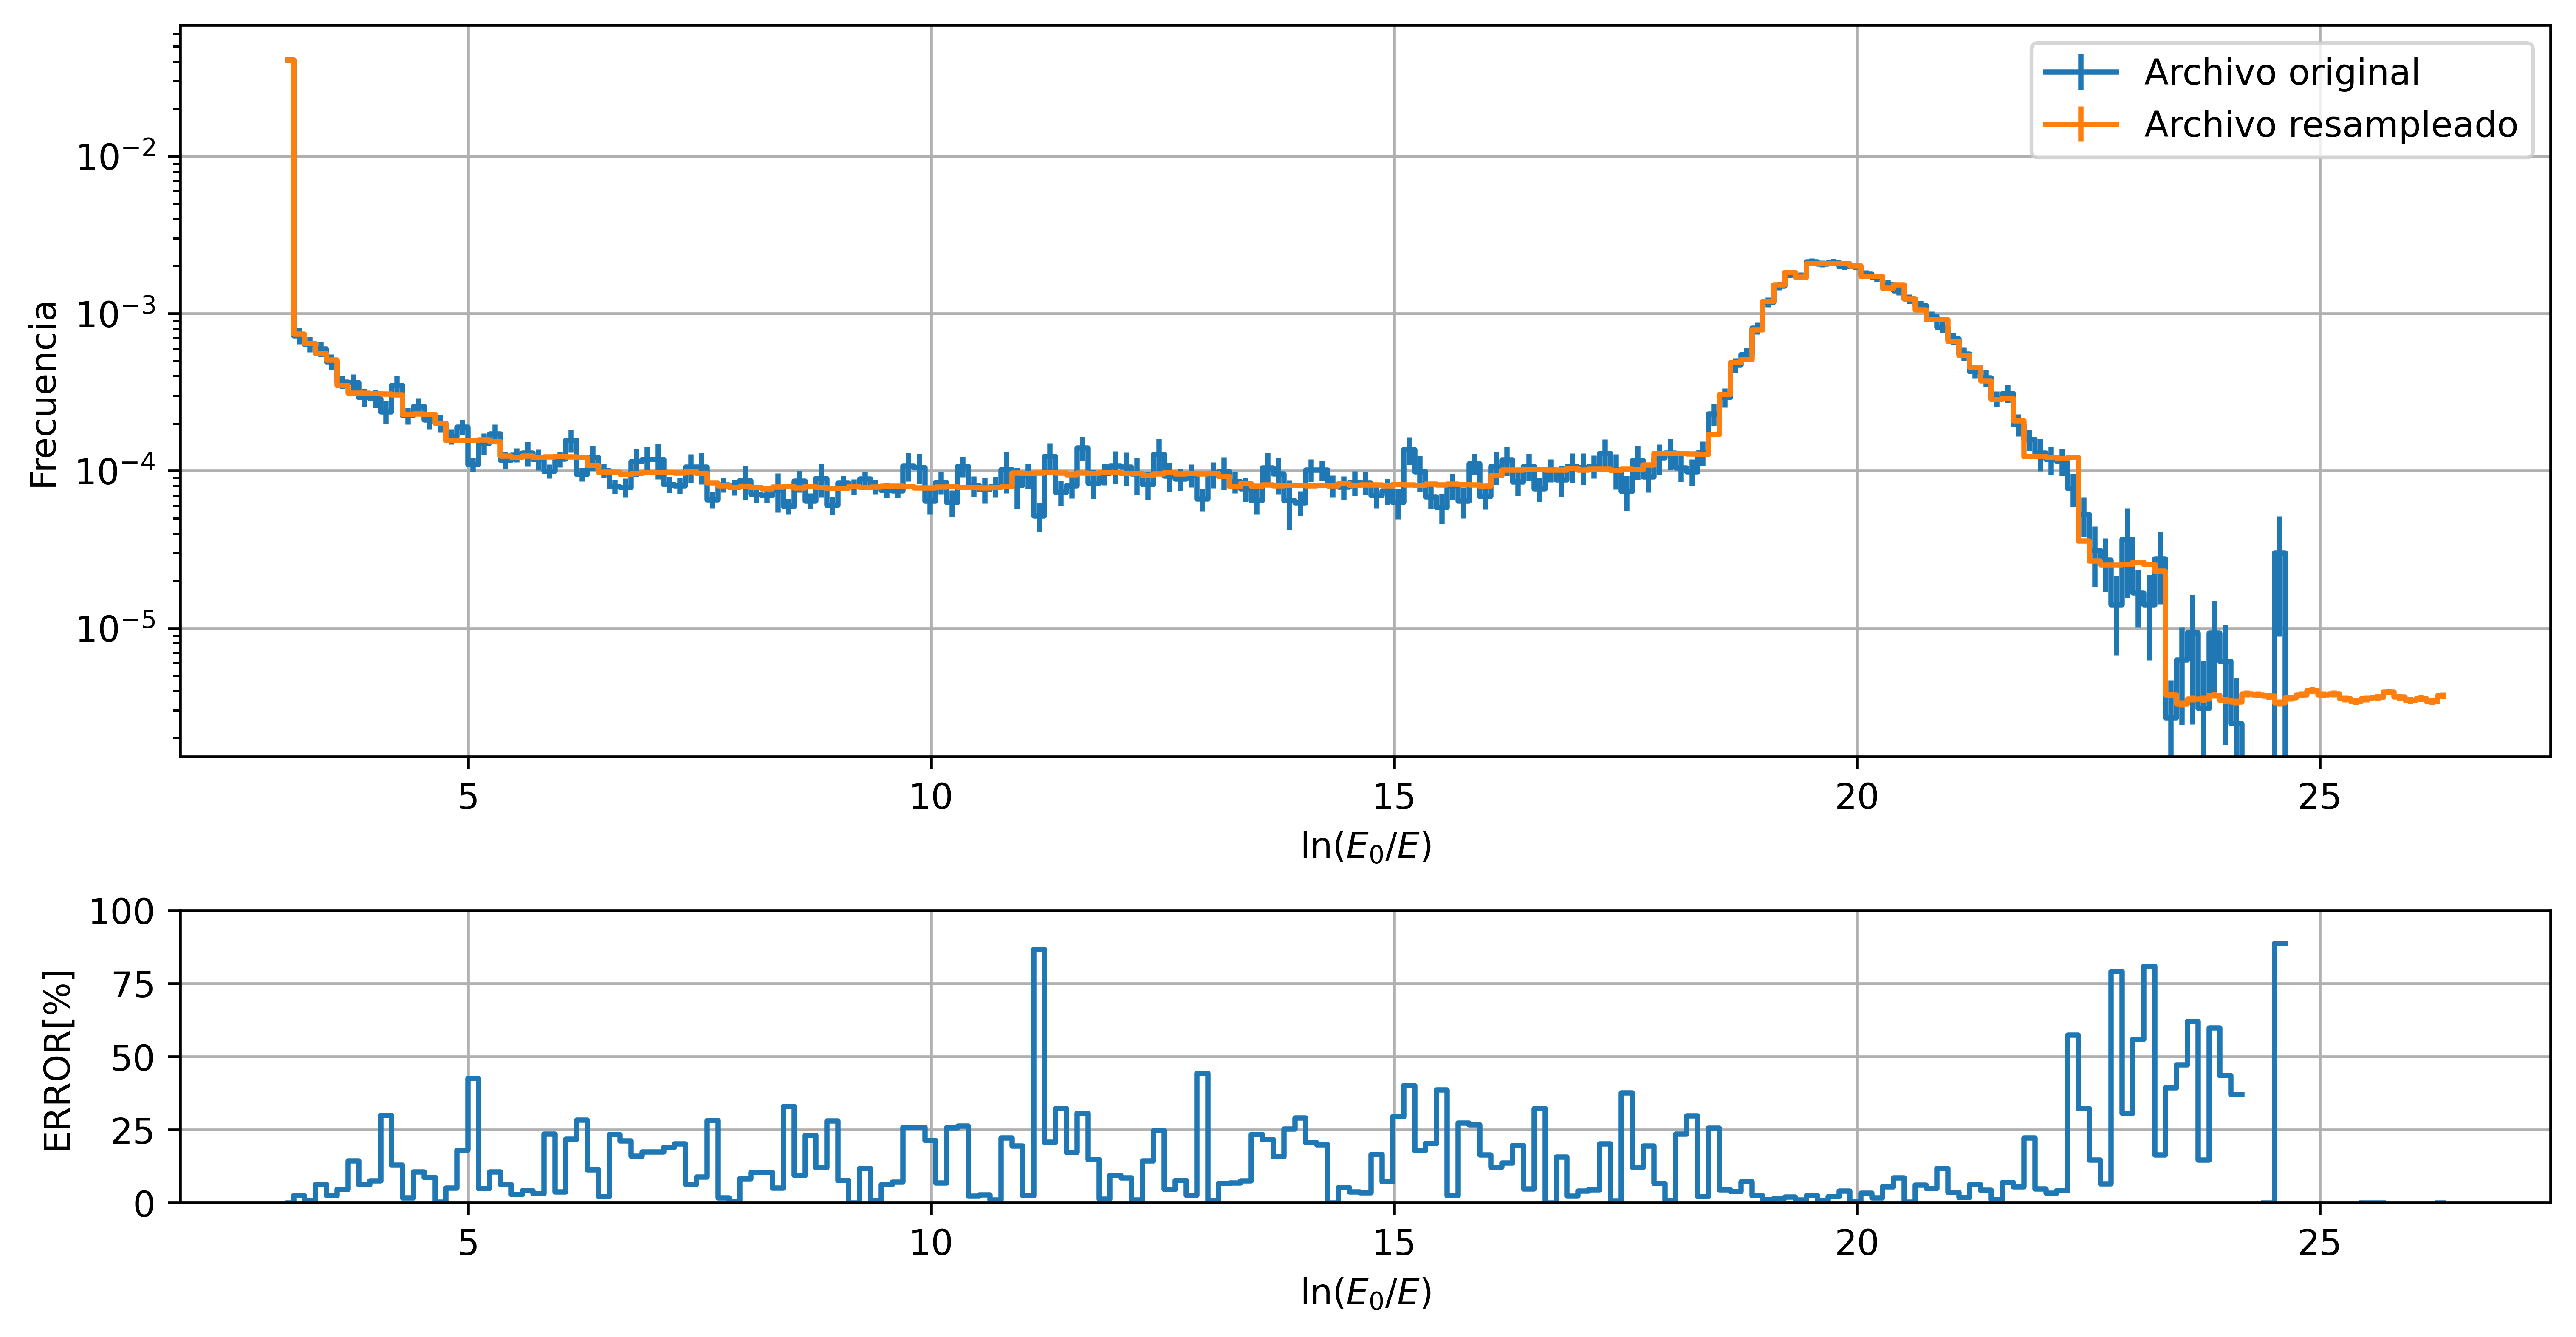
\includegraphics[width=\textwidth]{let_4.png}
    \caption{Distribución remuestreada de letargía para el caso de bineado adaptativo con borde manual en la zona de letargía correspondiente a una energía de $E = 1~MeV$.}
    \label{fig:let_4}
\end{figure}

\subsection{Distribuciones de $\mu$}
Se analizan a continuación las distribuciones remuestreadas de la variable direccional $\mu = \cos(\theta)$, obtenidas mediante las 4 configuraciones analizadas. Se evalúa la capacidad de cada método para representar adecuadamente la delta asociada a partículas colimadas ($\mu = 1$) y el comportamiento general de la distribución.

En la Figura \ref{fig:mu_1}, correspondiente al caso 1 de bineado uniforme sin bordes manuales, se observa que la delta en $\mu = 1$ es reemplazada por un escalón, debido a que el bin abarca toda la región colimada. Este efecto deteriora significativamente la representación en esa zona. Sin embargo, el resto de la distribución es tratada de forma aceptable, suavizando la distribución.

En la Figura \ref{fig:mu_2}, se introduce un borde manual para formar un bin de ancho $10^{-9}$ en la zona de $\mu = 1$, lo que permite aislar correctamente la región colimada. Como resultado, se recupera la forma tipo delta en esa zona, y se mantiene una buena representación en el resto de la distribución.

\begin{figure}[H]
    \centering
    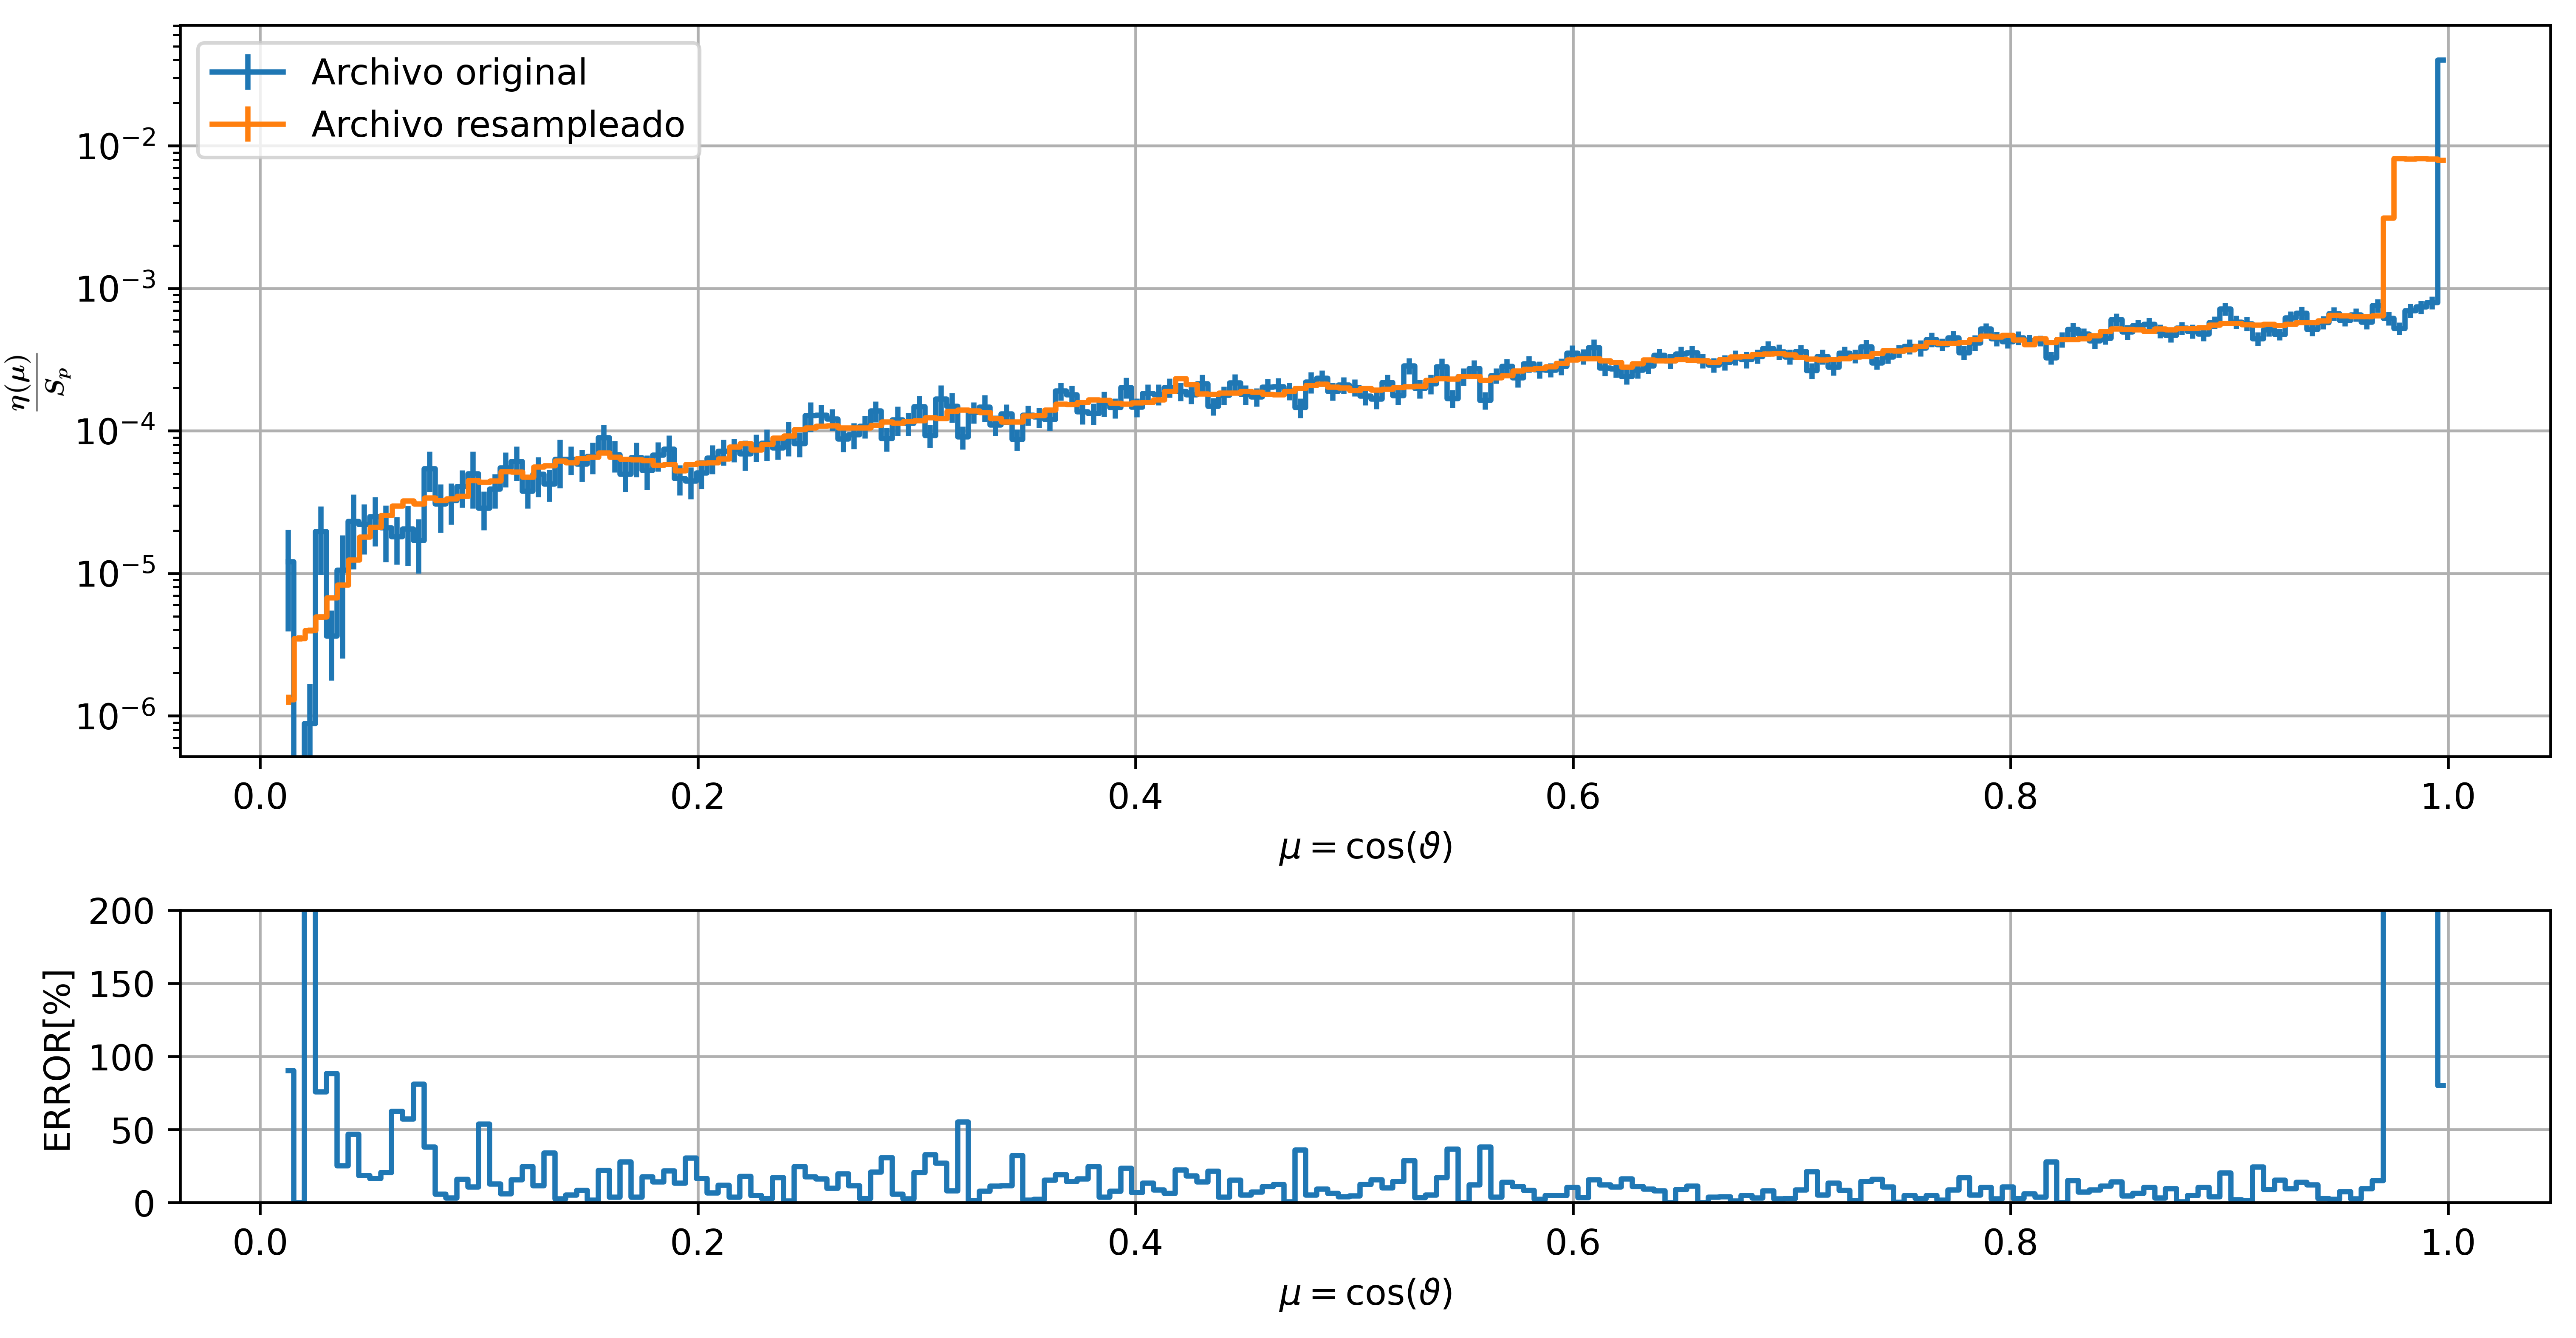
\includegraphics[width=\textwidth]{mu_1.png}
    \caption{Distribución remuestreada de $\mu$ para el caso 1 de bineado uniforme sin bordes manuales.}
    \label{fig:mu_1}
\end{figure}

\begin{figure}[H]
    \centering
    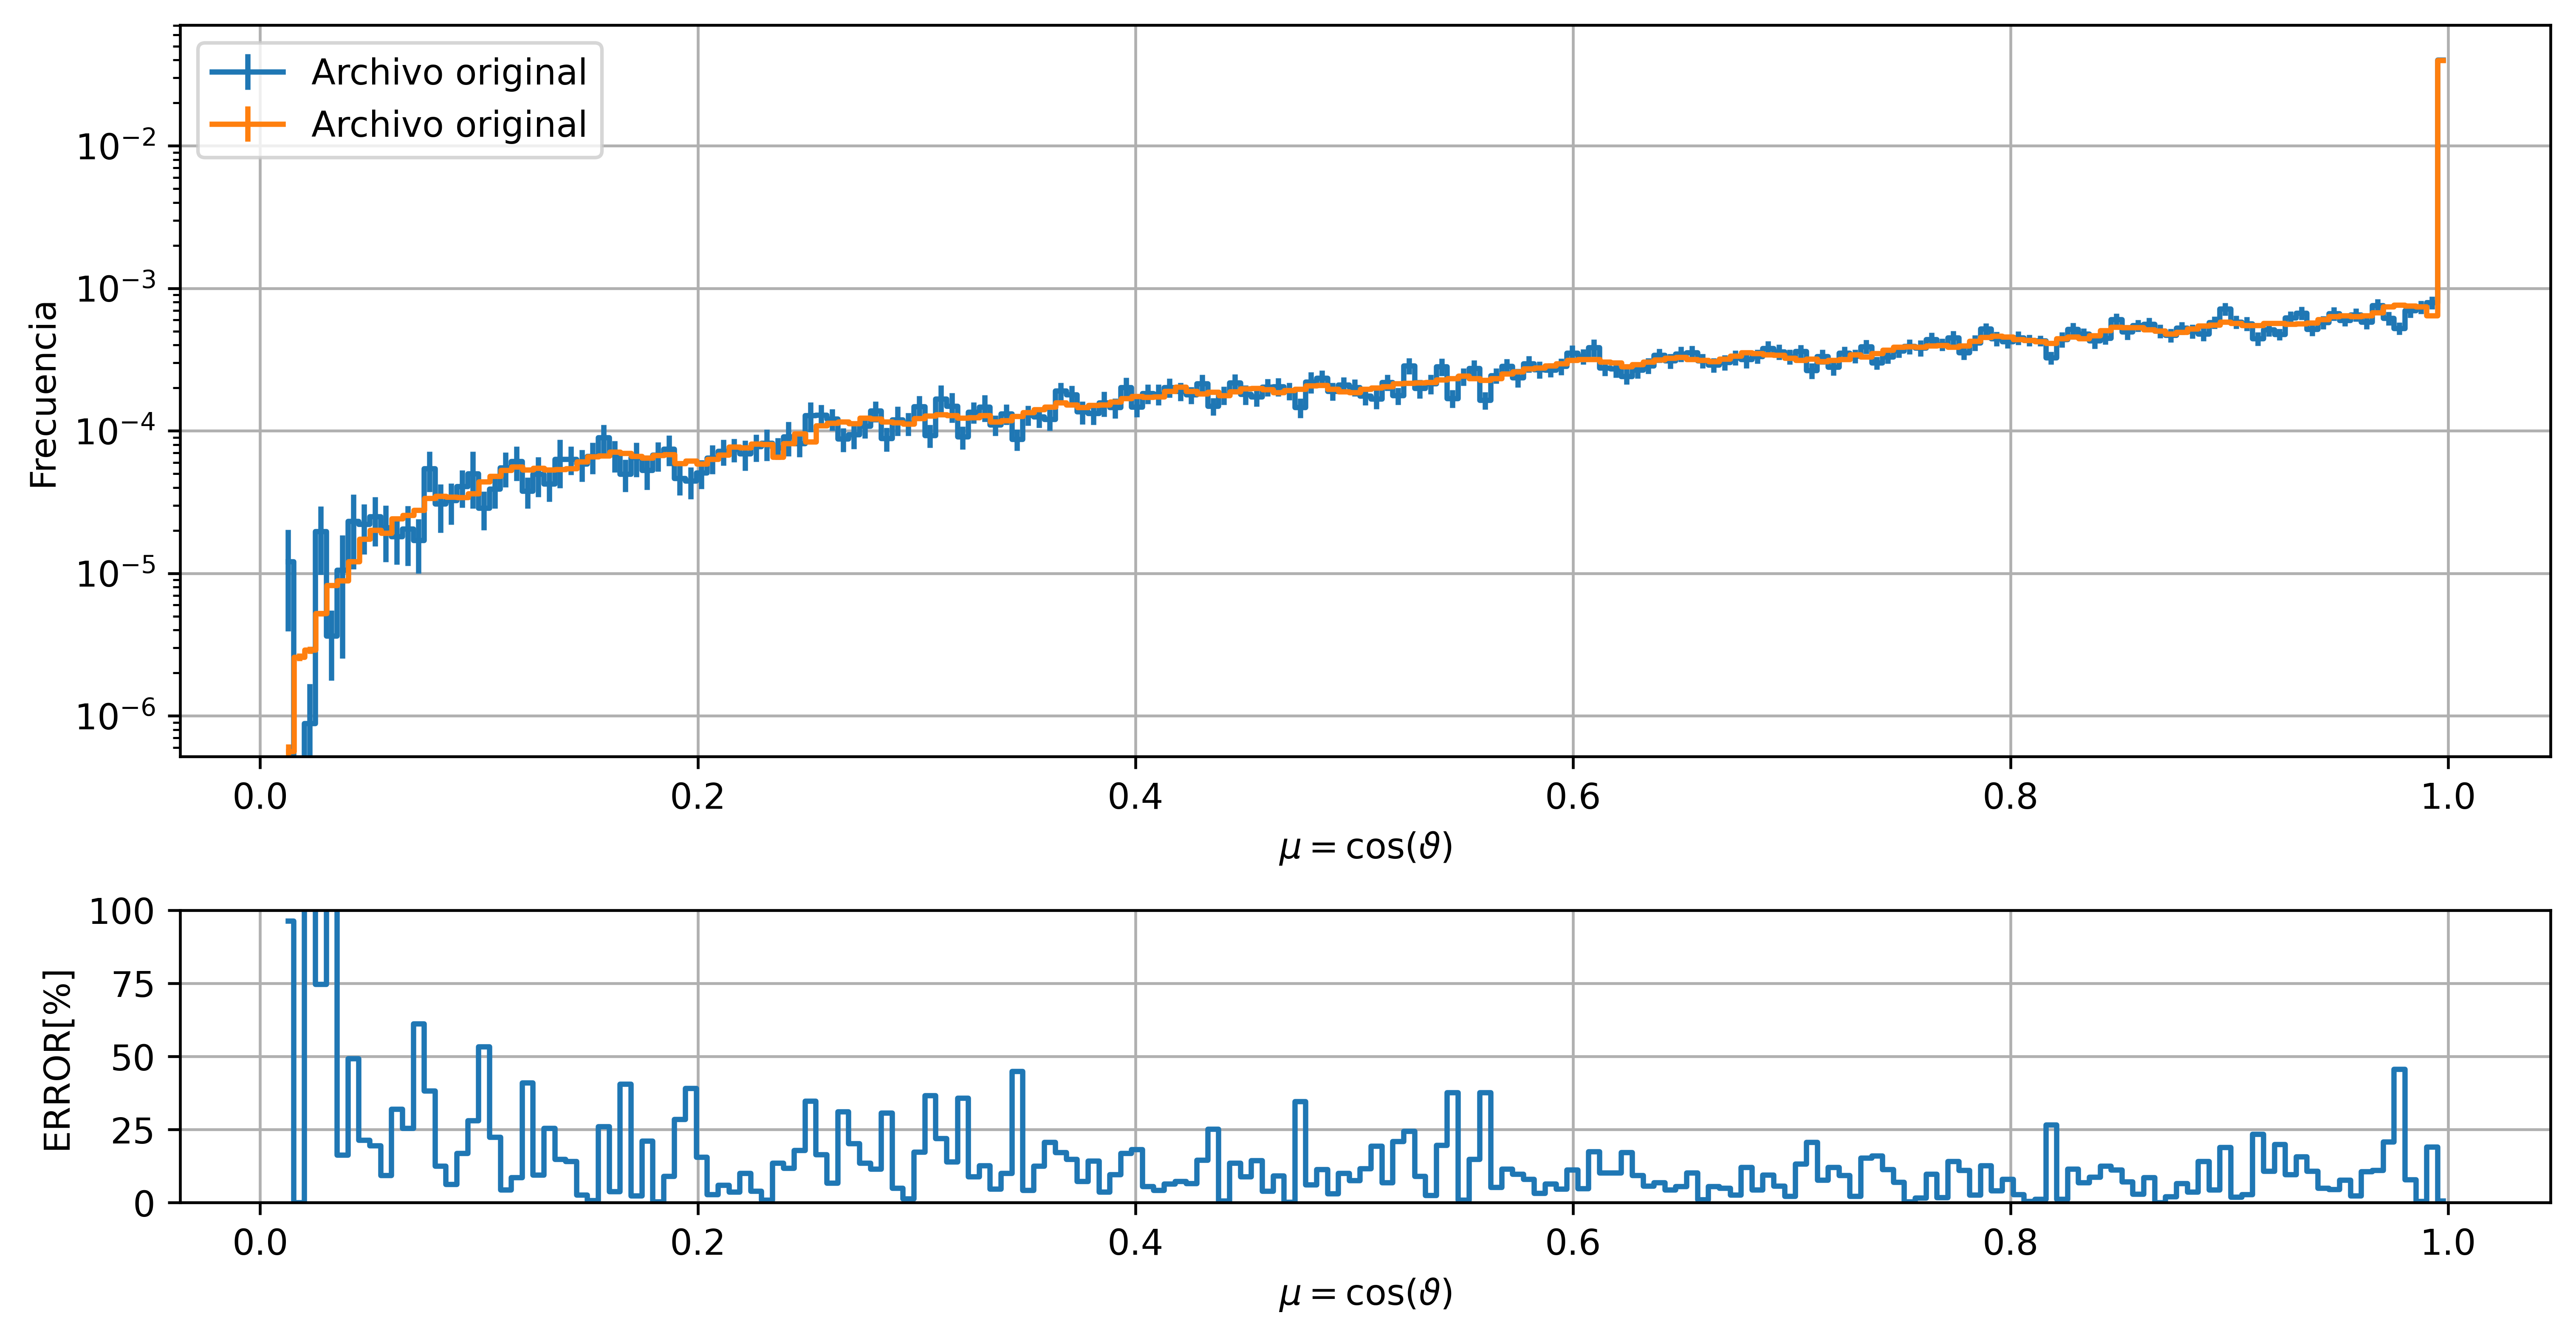
\includegraphics[width=\textwidth]{mu_2.png}
    \caption{Distribución remuestreada de $\mu$ para el caso 2 de bineado uniforme con borde manual en $\mu \approx 1$.}
    \label{fig:mu_2}
\end{figure}

La Figura \ref{fig:mu_3} muestra los resultados del caso 3 obtenidos con histogramas adaptativos sin bordes manuales. En este caso, el método logra seguir de manera precisa la forma original, tanto en la delta como en el resto de la distribución. Sin embargo, este seguimiento resulta excesivo, reproduciendo el ruido estadístico del archivo de partículas original, lo cual no es deseable. Este efecto se debe a la elevada cantidad de bines asignados: como $\mu$ es la cuarta variable en el orden de segmentación, se trabaja sobre subconjuntos reducidos de partículas, lo cual hace que 36 bines resulte una resolución desproporcionada.

\begin{figure}[H]
    \centering
    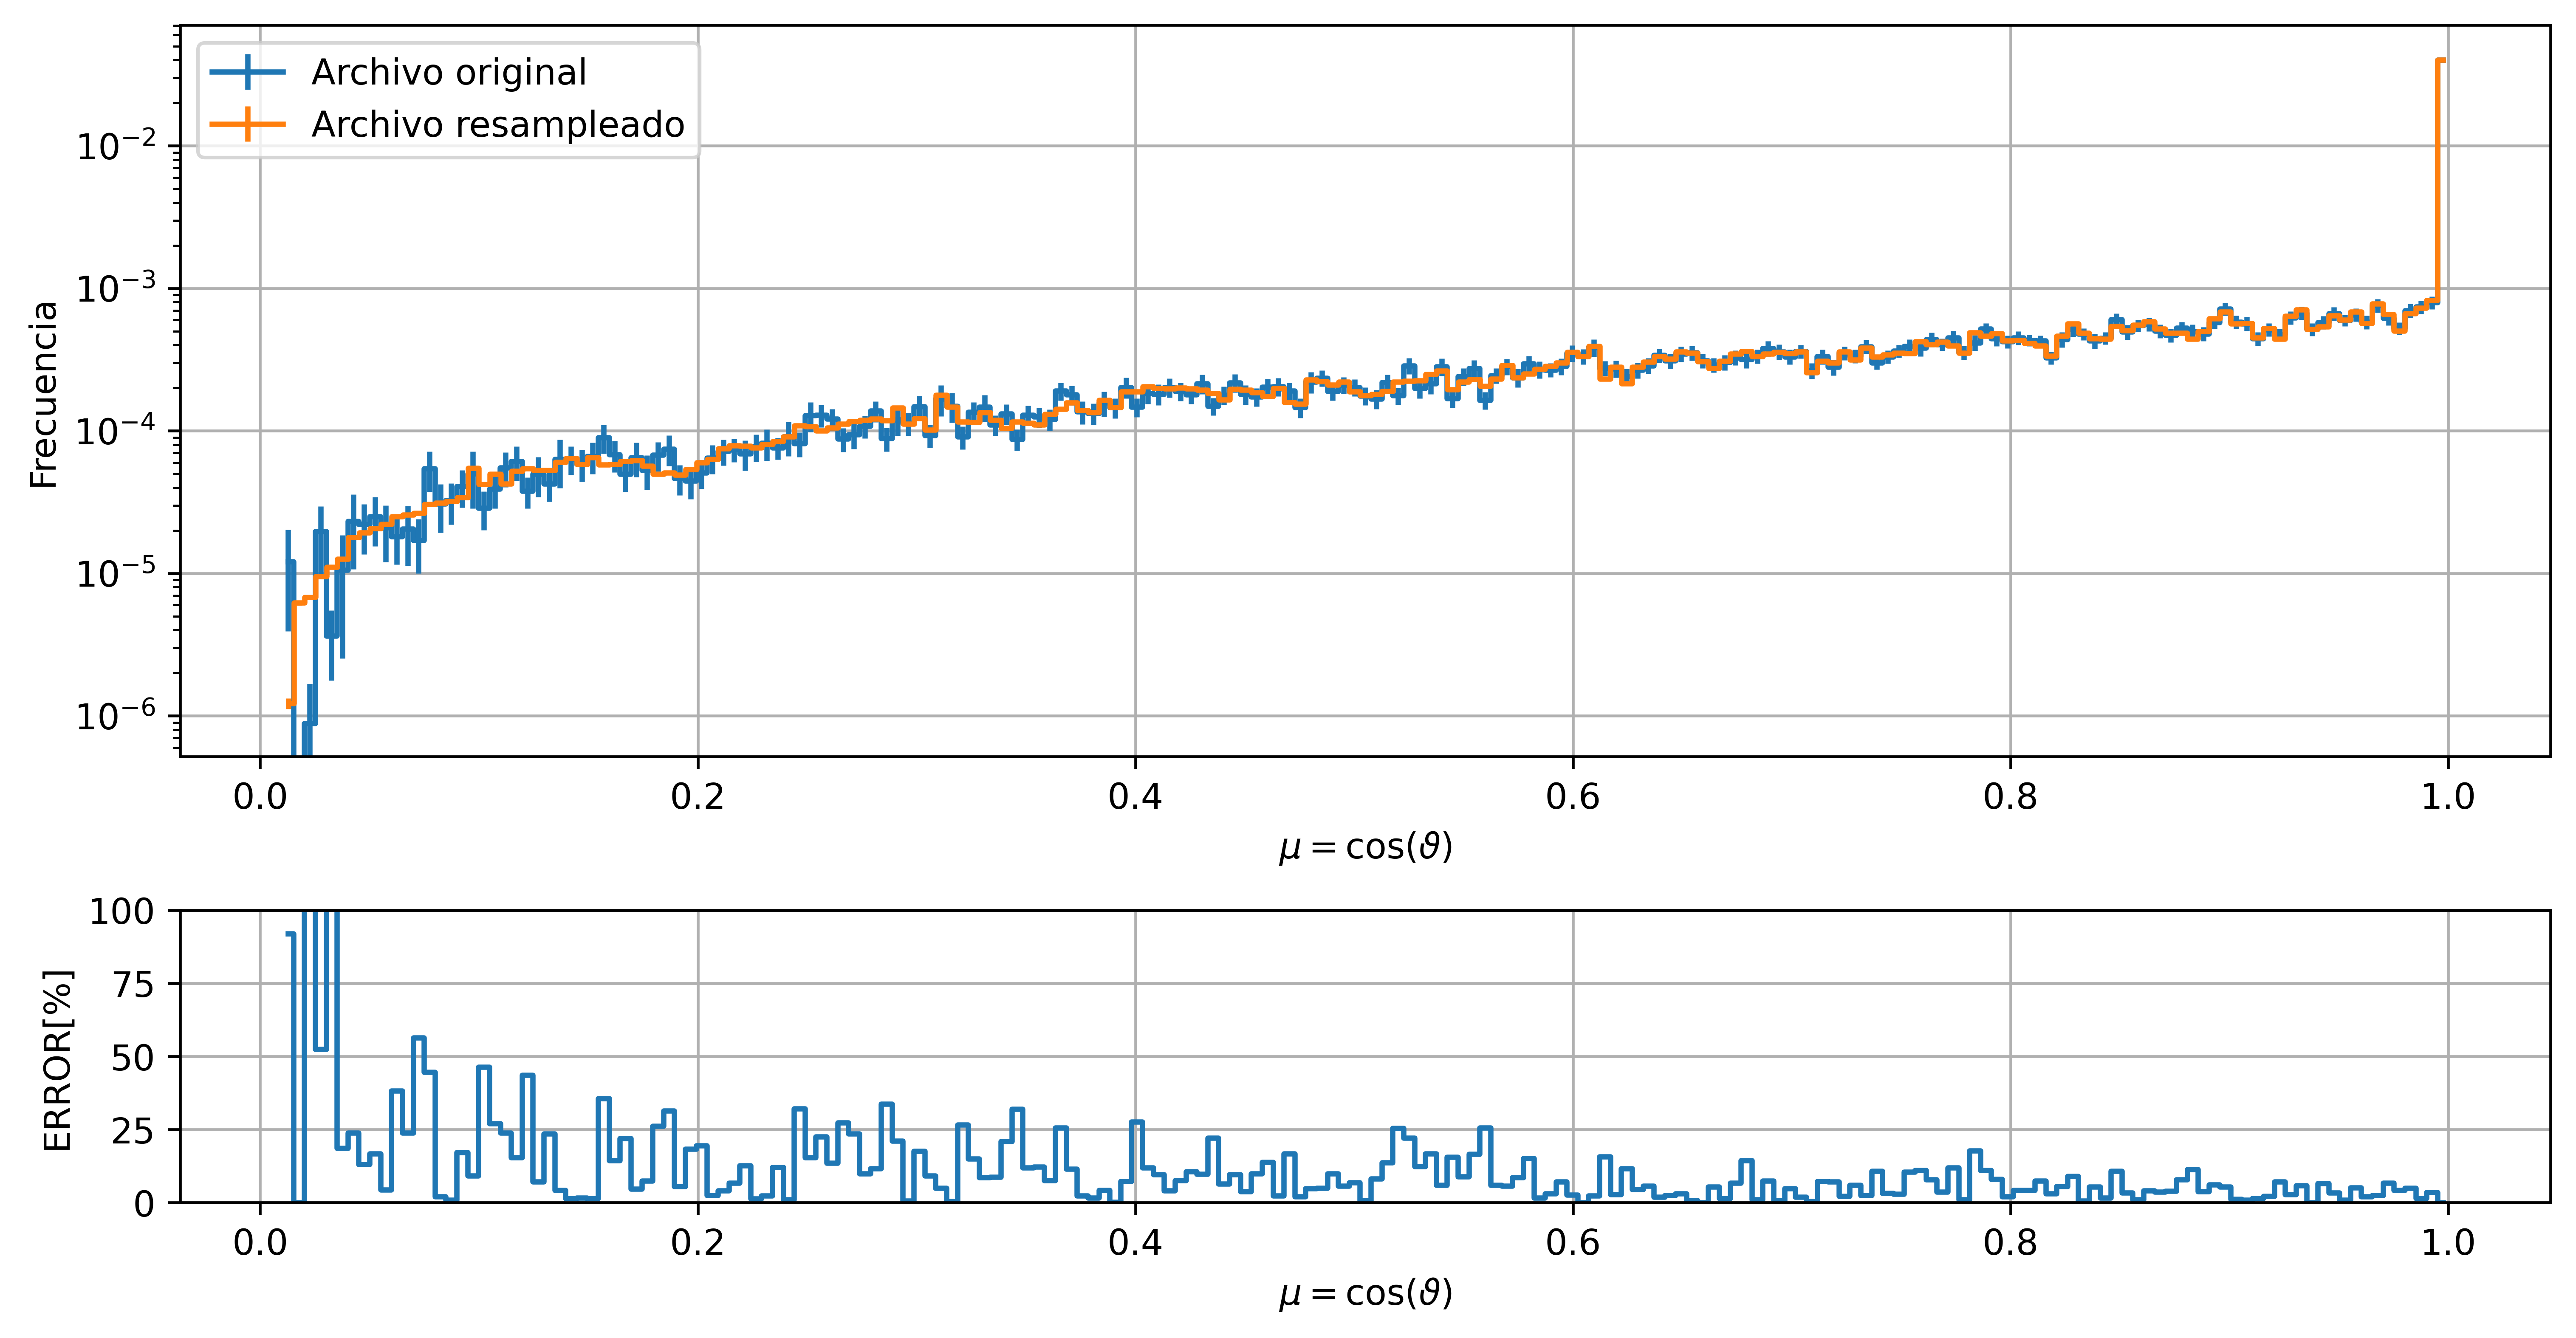
\includegraphics[width=\textwidth]{mu_3.png}
    \caption{Distribución remuestreada de $\mu$ para el caso 3 de bineado adaptativo sin bordes manuales.}
    \label{fig:mu_3}
\end{figure}

En la Figura \ref{fig:mu_4}, se incorpora un borde manual en la zona colimada, pero no se observan cambios relevantes con respecto al caso anterior. Esto evidencia que el algoritmo adaptativo es capaz de detectar y segmentar adecuadamente esta región sin intervención adicional, siempre que la resolución no sea excesiva.

\begin{figure}[H]
    \centering
    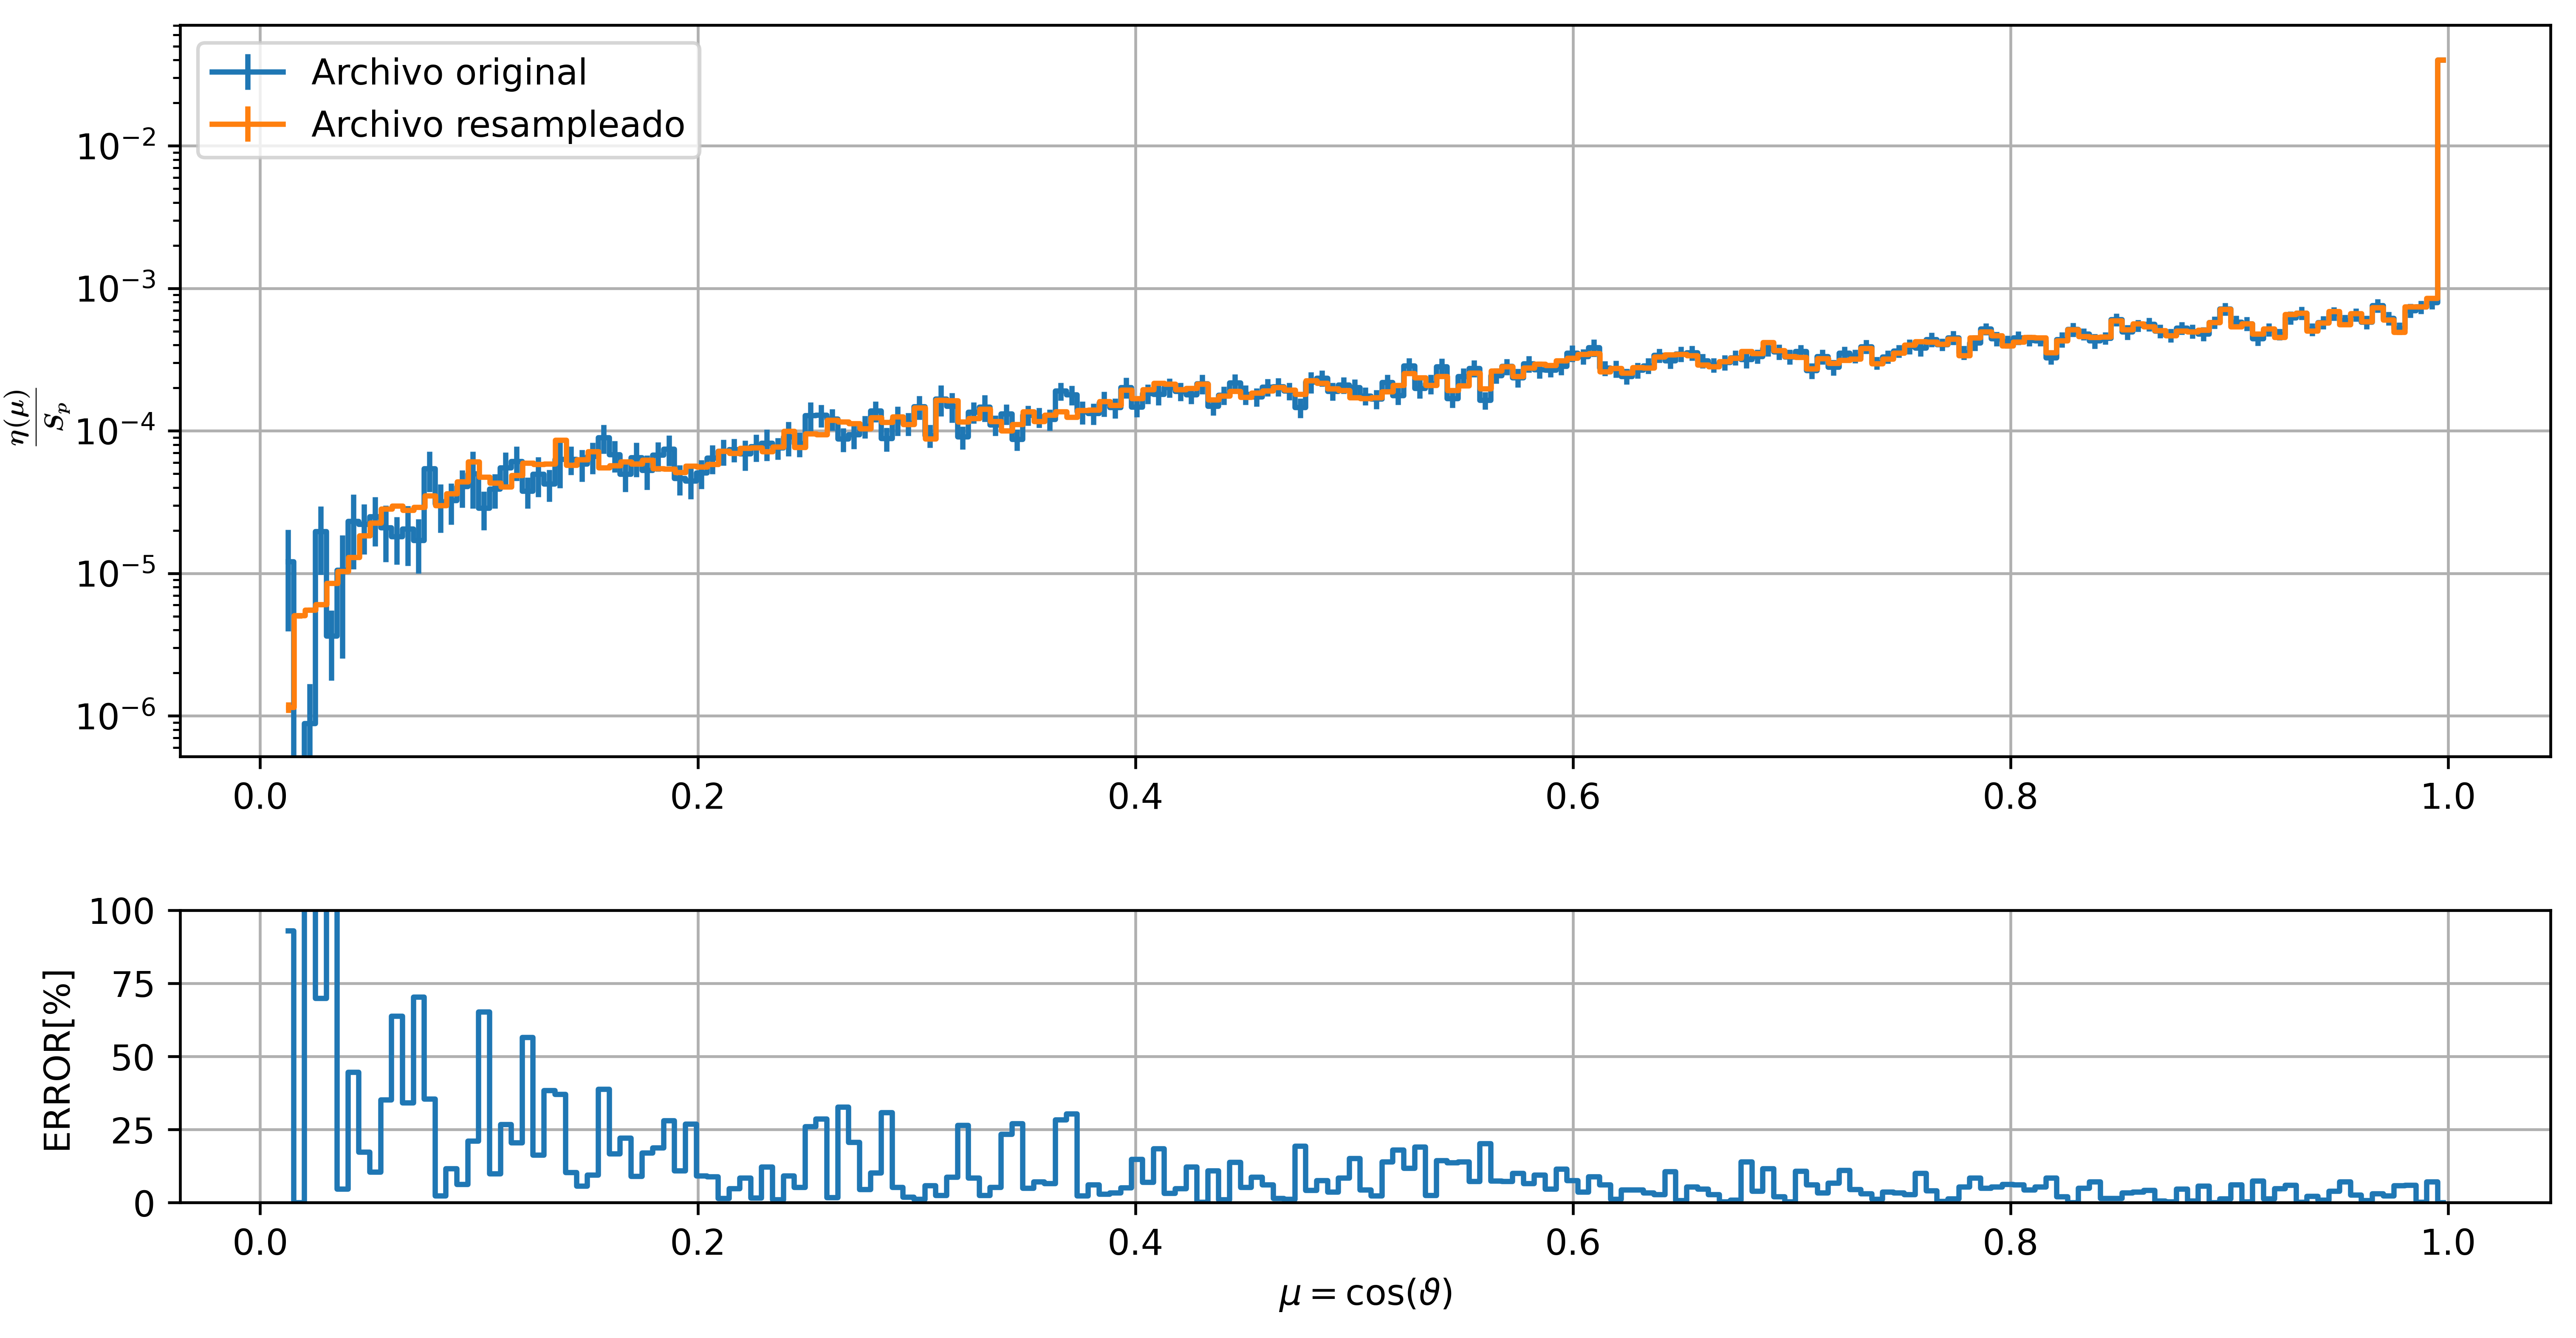
\includegraphics[width=\textwidth]{mu_4.png}
    \caption{Distribución remuestreada de $\mu$ para el caso 4 de bineado adaptativo con borde manual en $\mu \approx 1$.}
    \label{fig:mu_4}
\end{figure}

\subsection{Distribuciones espaciales $X$–$Y$}

En esta sección se detallan las distribuciones espaciales en el plano $X$–$Y$ para las 4 configuraciones analizadas. Se evalúa particularmente la capacidad de cada método para representar correctamente la geometría del sistema, especialmente en torno a la interfaz agua–vacío definida por el tubo.
    
En la Figura \ref{fig:xy_1}, correspondiente al caso 1 de bineado uniforme sin bordes, se observa un suavizado de la estadística entre regiones físicamente distintas. En particular, aparecen partículas remuestreadas en el agua que originalmente deberían haberse generado dentro del tubo de vacío. Este efecto se debe a que los histogramas uniformes no capturan la interfaz geométrica del sistema: un mismo bin puede contener partículas tanto dentro como fuera del tubo, y al remuestrear, se reparten en ambas regiones.

\begin{figure}[H]
    \centering
    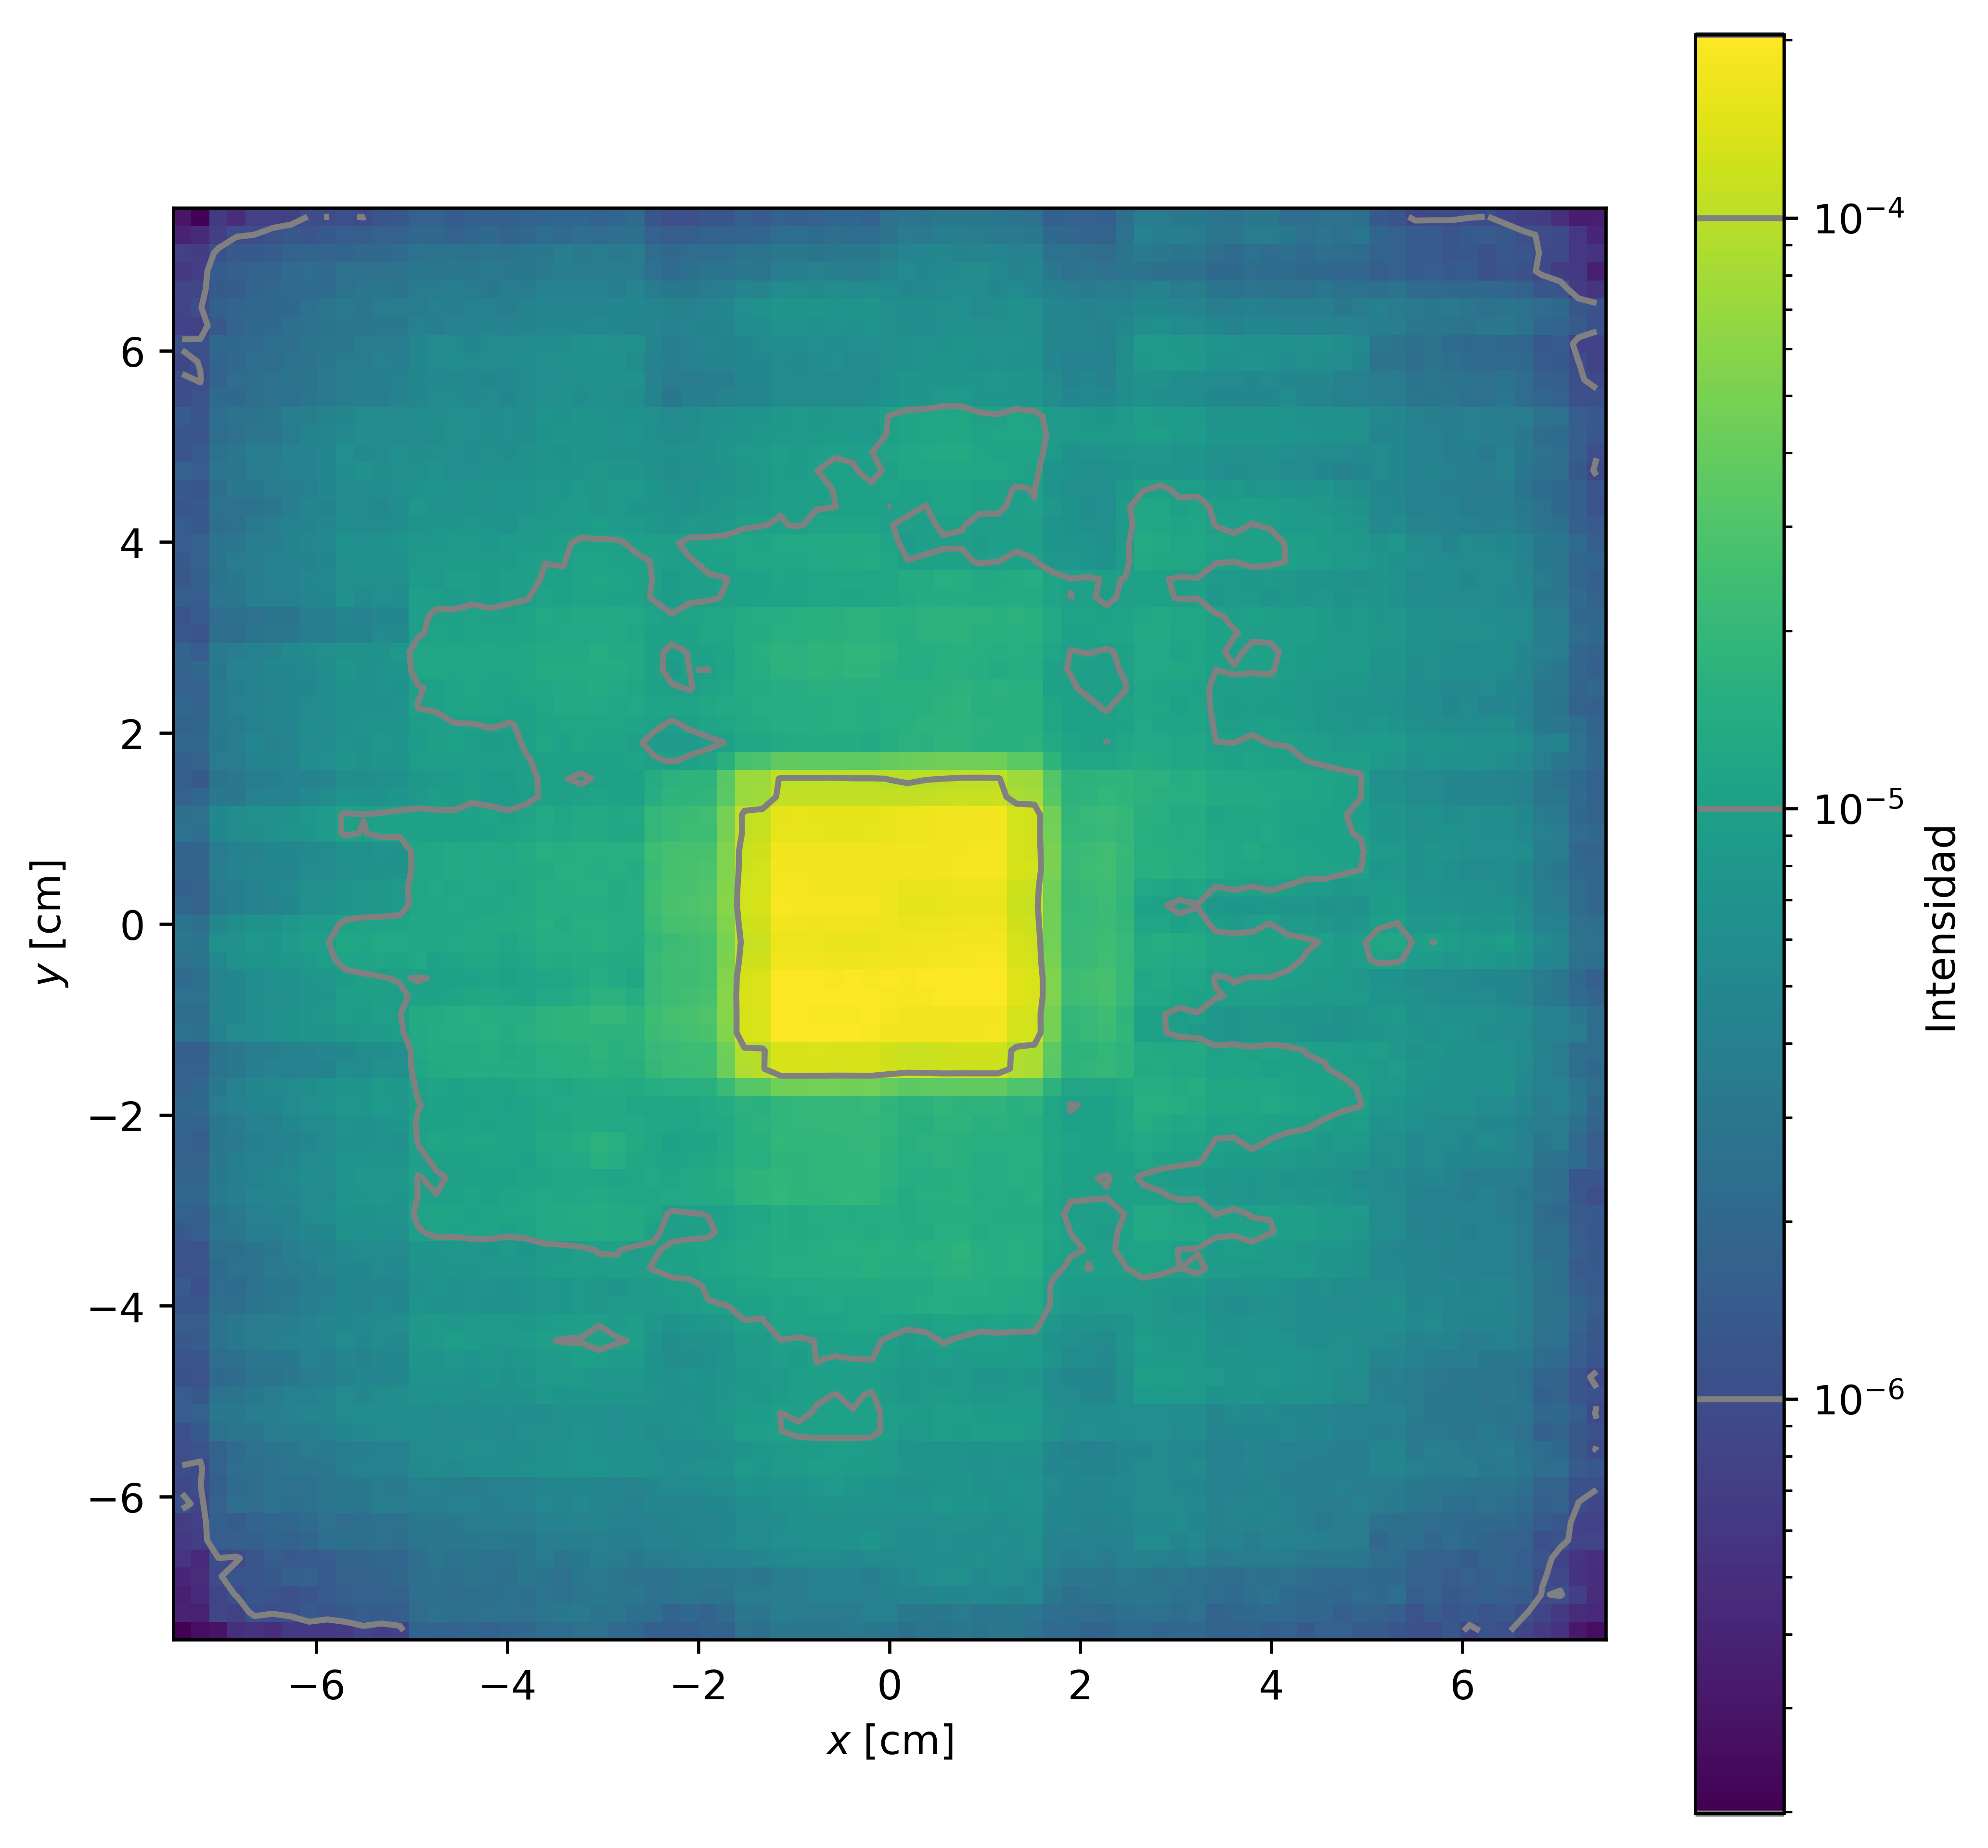
\includegraphics[width=0.6\textwidth]{xy_1.png}
    \caption{Distribución remuestreada en el plano $X$–$Y$ para el caso 1 de bineado uniforme sin bordes manuales.}
    \label{fig:xy_1}
\end{figure}

En la Figura \ref{fig:xy_2}, se incorporan bordes manuales para delimitar la región correspondiente al canal de vacío. Este ajuste mejora la segmentación espacial, concentrando la estadística dentro del tubo y evitando que partículas aparezcan en el agua. Sin embargo, se observa una estructura cuadriculada en el agua, debido a la baja estadística original combinada con la discretización forzada en grupos debido al bineado uniforme de los histogramas macro.

\begin{figure}[H]
    \centering
    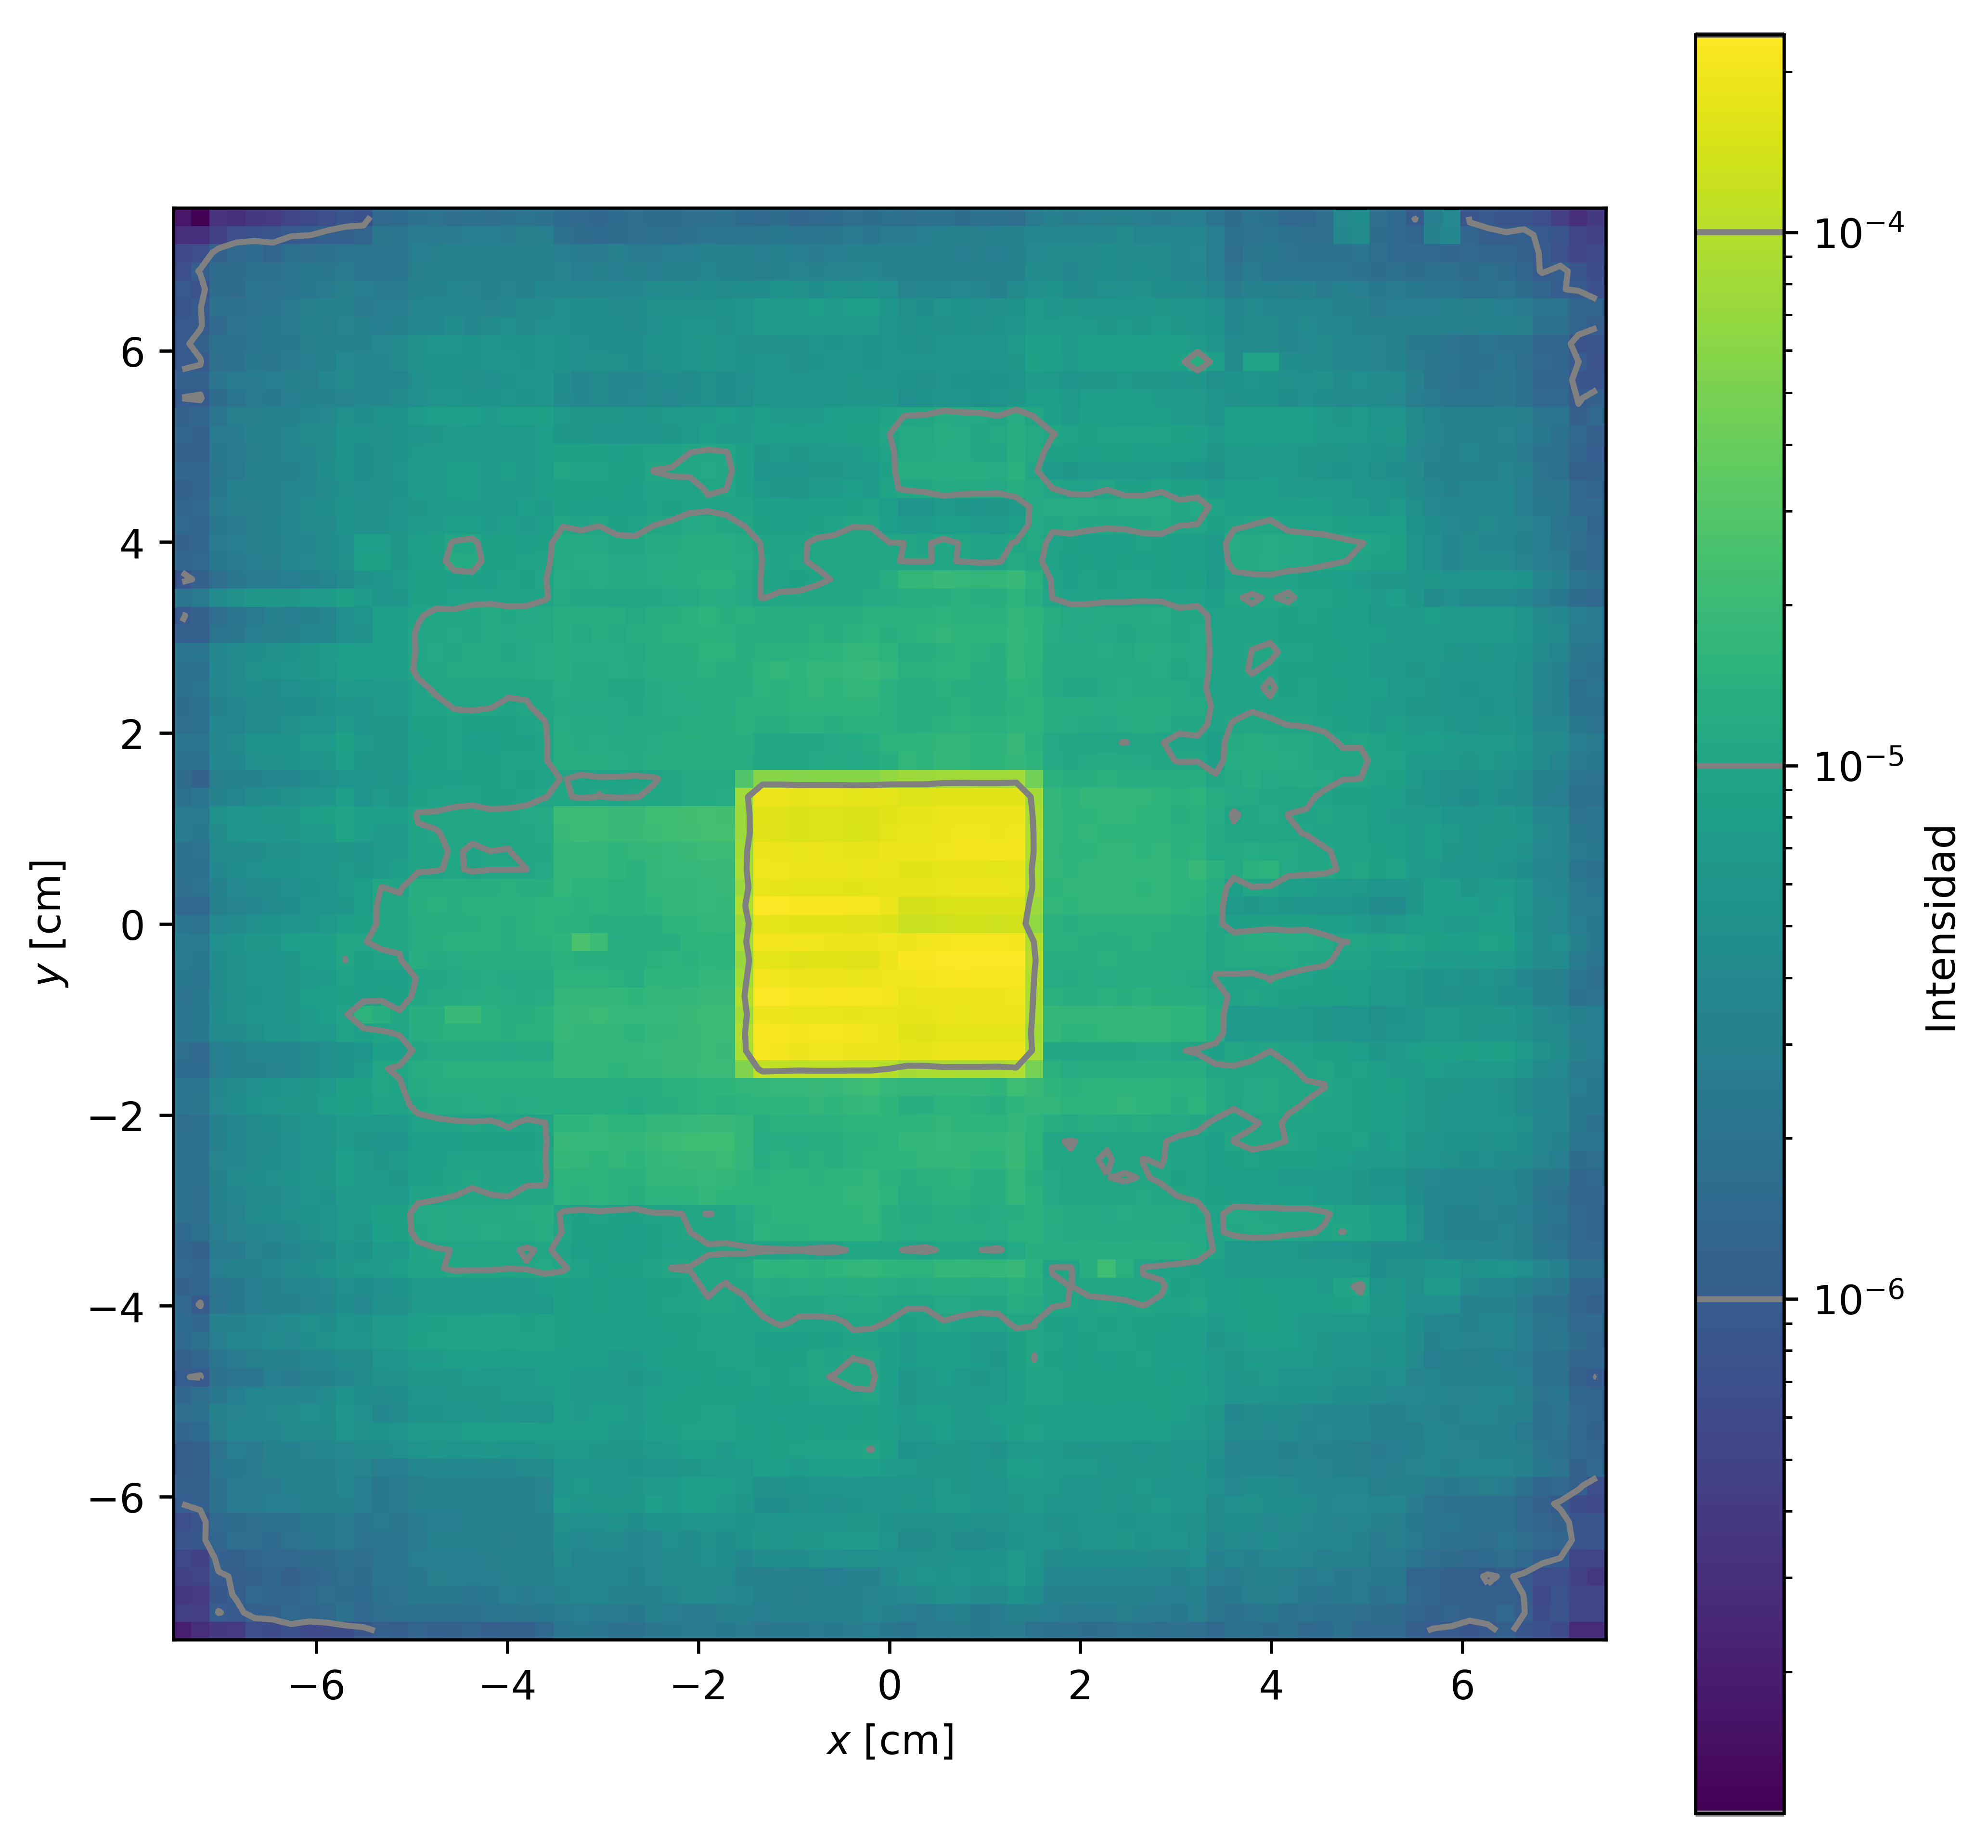
\includegraphics[width=0.6\textwidth]{xy_2.png}
    \caption{Distribución remuestreada en el plano $X$–$Y$ para el caso 2 de bineado uniforme con bordes manuales en la interfaz agua–vacío.}
    \label{fig:xy_2}
\end{figure}

La Figura \ref{fig:xy_3} presenta el resultado del caso 3 de bineado adaptativo sin bordes definidos por el usuario. En este caso, se observa que el método logra capturar adecuadamente la transición entre regiones, evitando la aparición de partículas en zonas del agua donde no correspondía. La distribución dentro del agua se muestra más homogénea que en el caso anterior, debido a que el algoritmo adaptativo no fuerza la segmentación en regiones con baja estadística.

\begin{figure}[H]
    \centering
    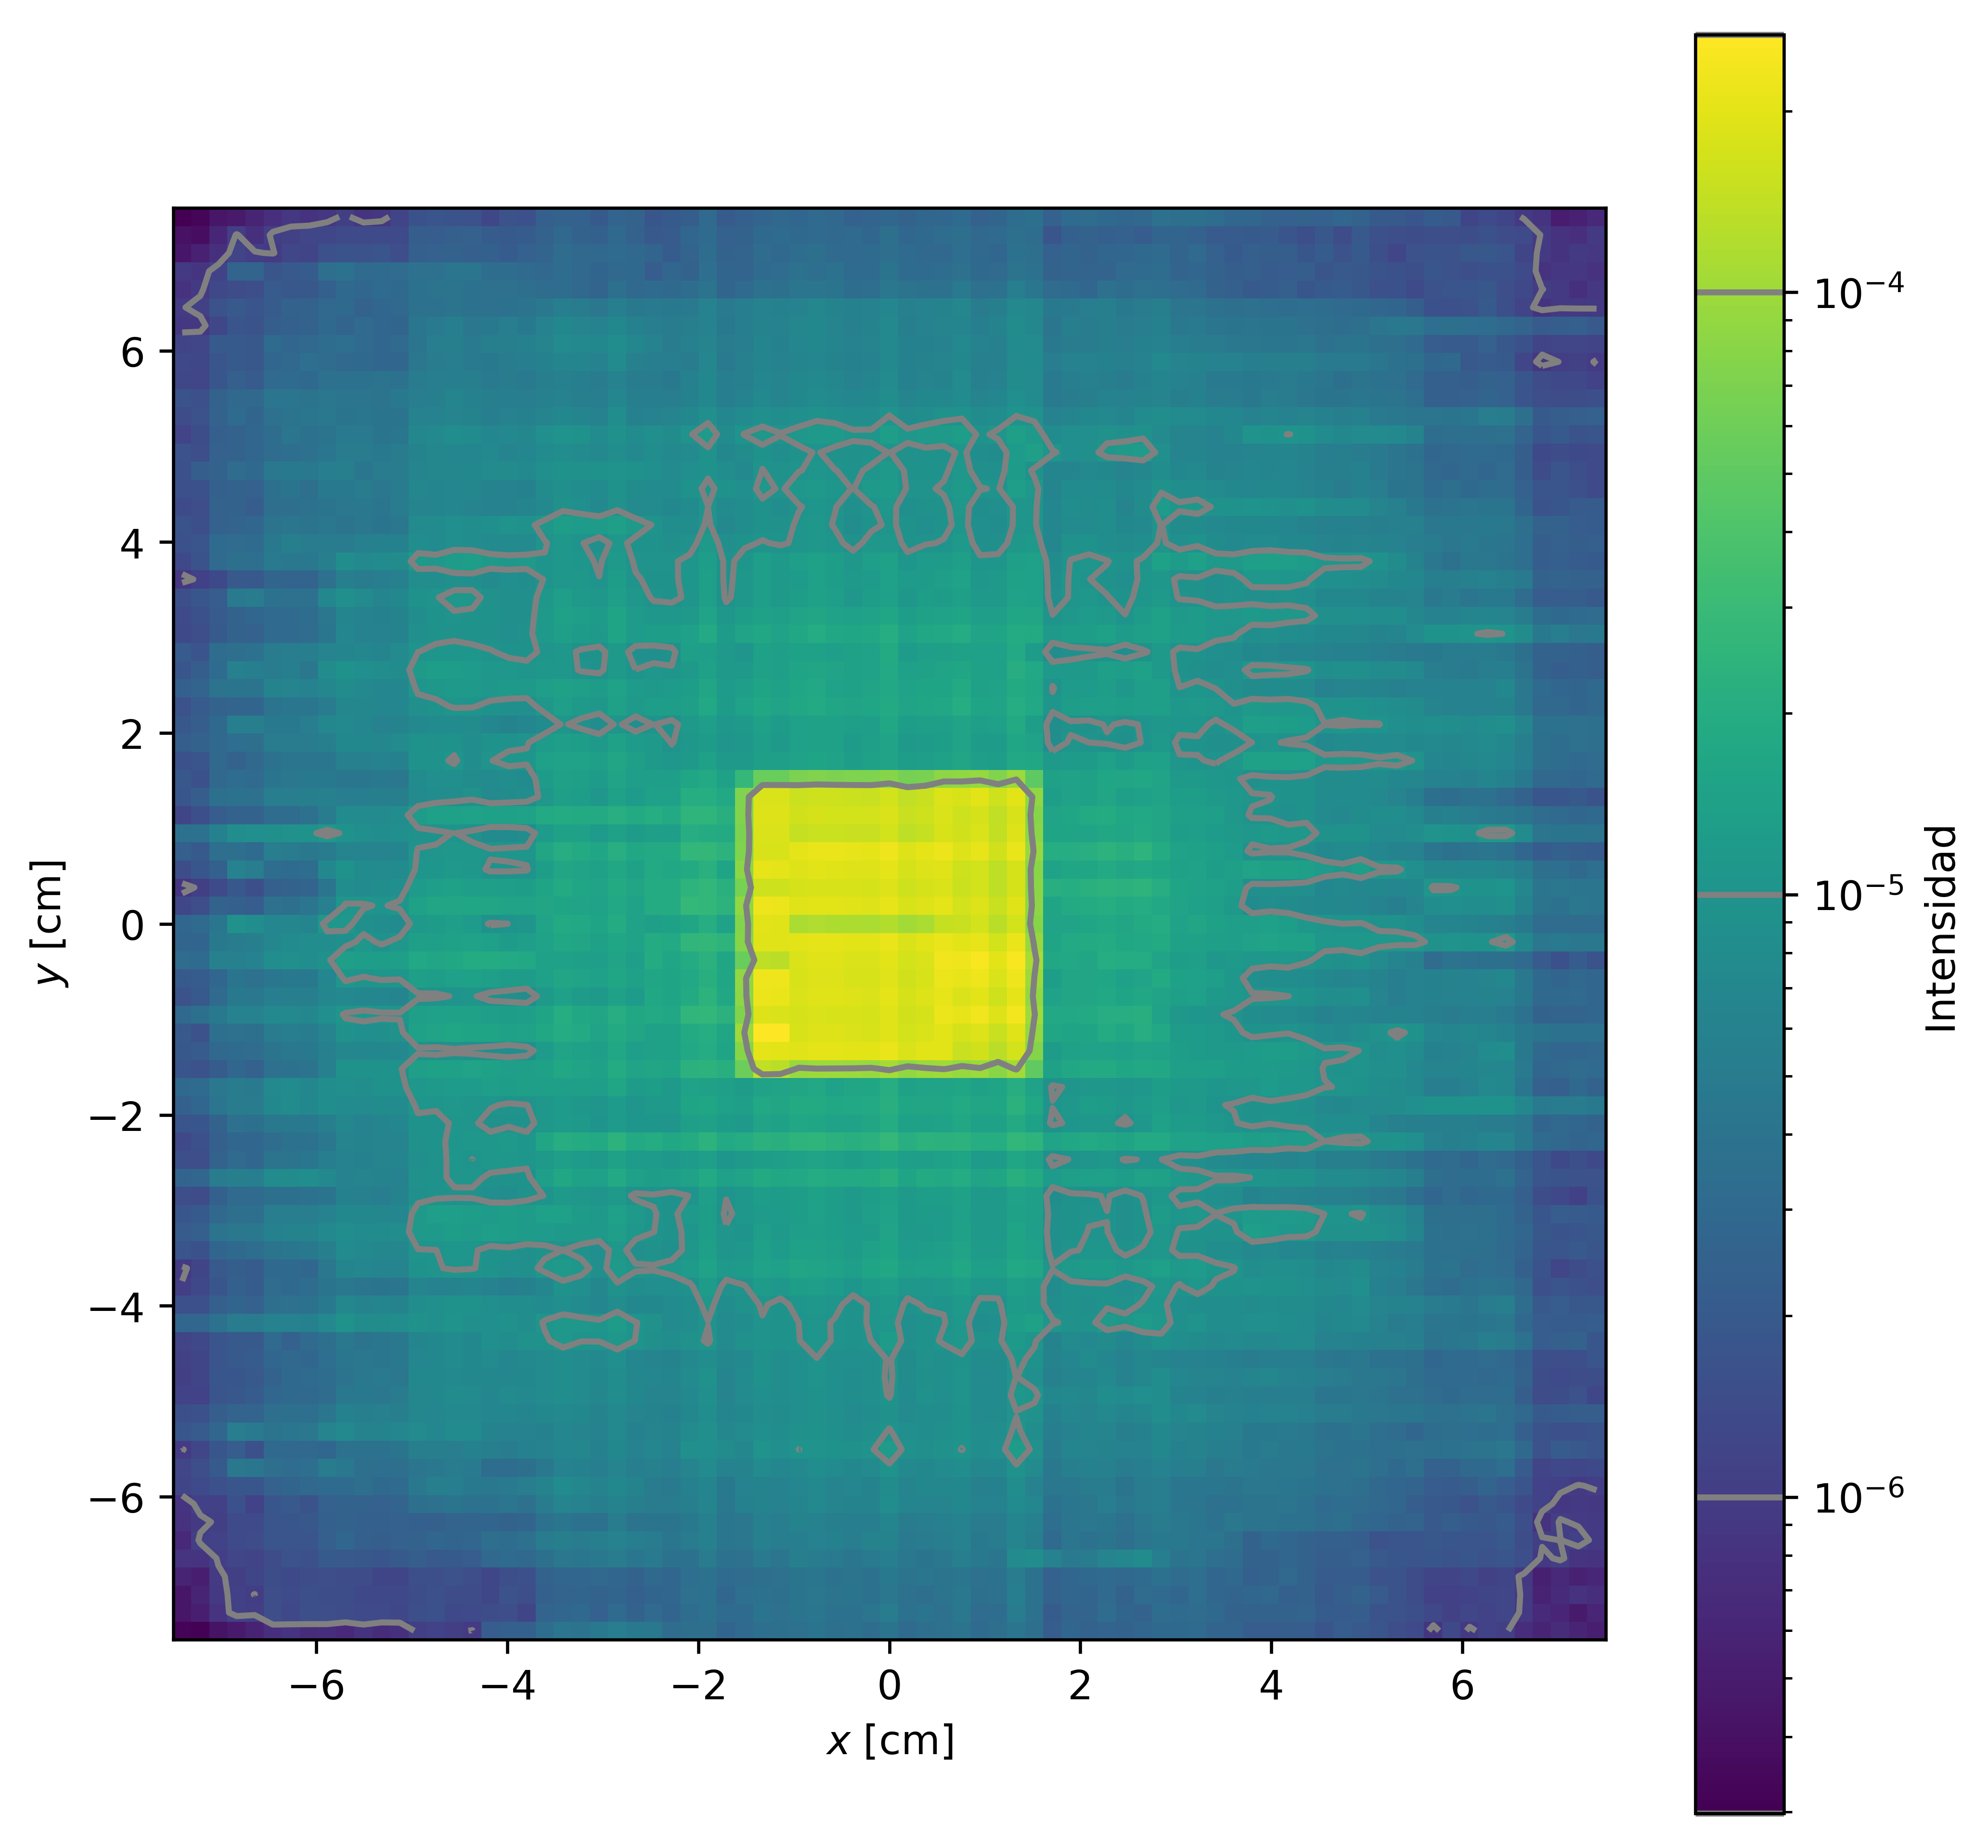
\includegraphics[width=0.6\textwidth]{xy_3.png}
    \caption{Distribución remuestreada en el plano $X$–$Y$ para el caso 3 de bineado adaptativo sin bordes manuales.}
    \label{fig:xy_3}
\end{figure}

En la Figura \ref{fig:xy_4}, se observa el caso 4 de bineado adaptativo con bordes definidos por el usuario en la interfaz. Si bien los resultados son visualmente similares a los del caso sin bordes, puede señalarse que aquí los límites del canal de vacío están representados de forma más precisa, dado que se han especificado explícitamente. No obstante, el método adaptativo sin bordes ya proporciona una aproximación razonable, por lo que la mejora en este caso es leve.

\begin{figure}[H]
    \centering
    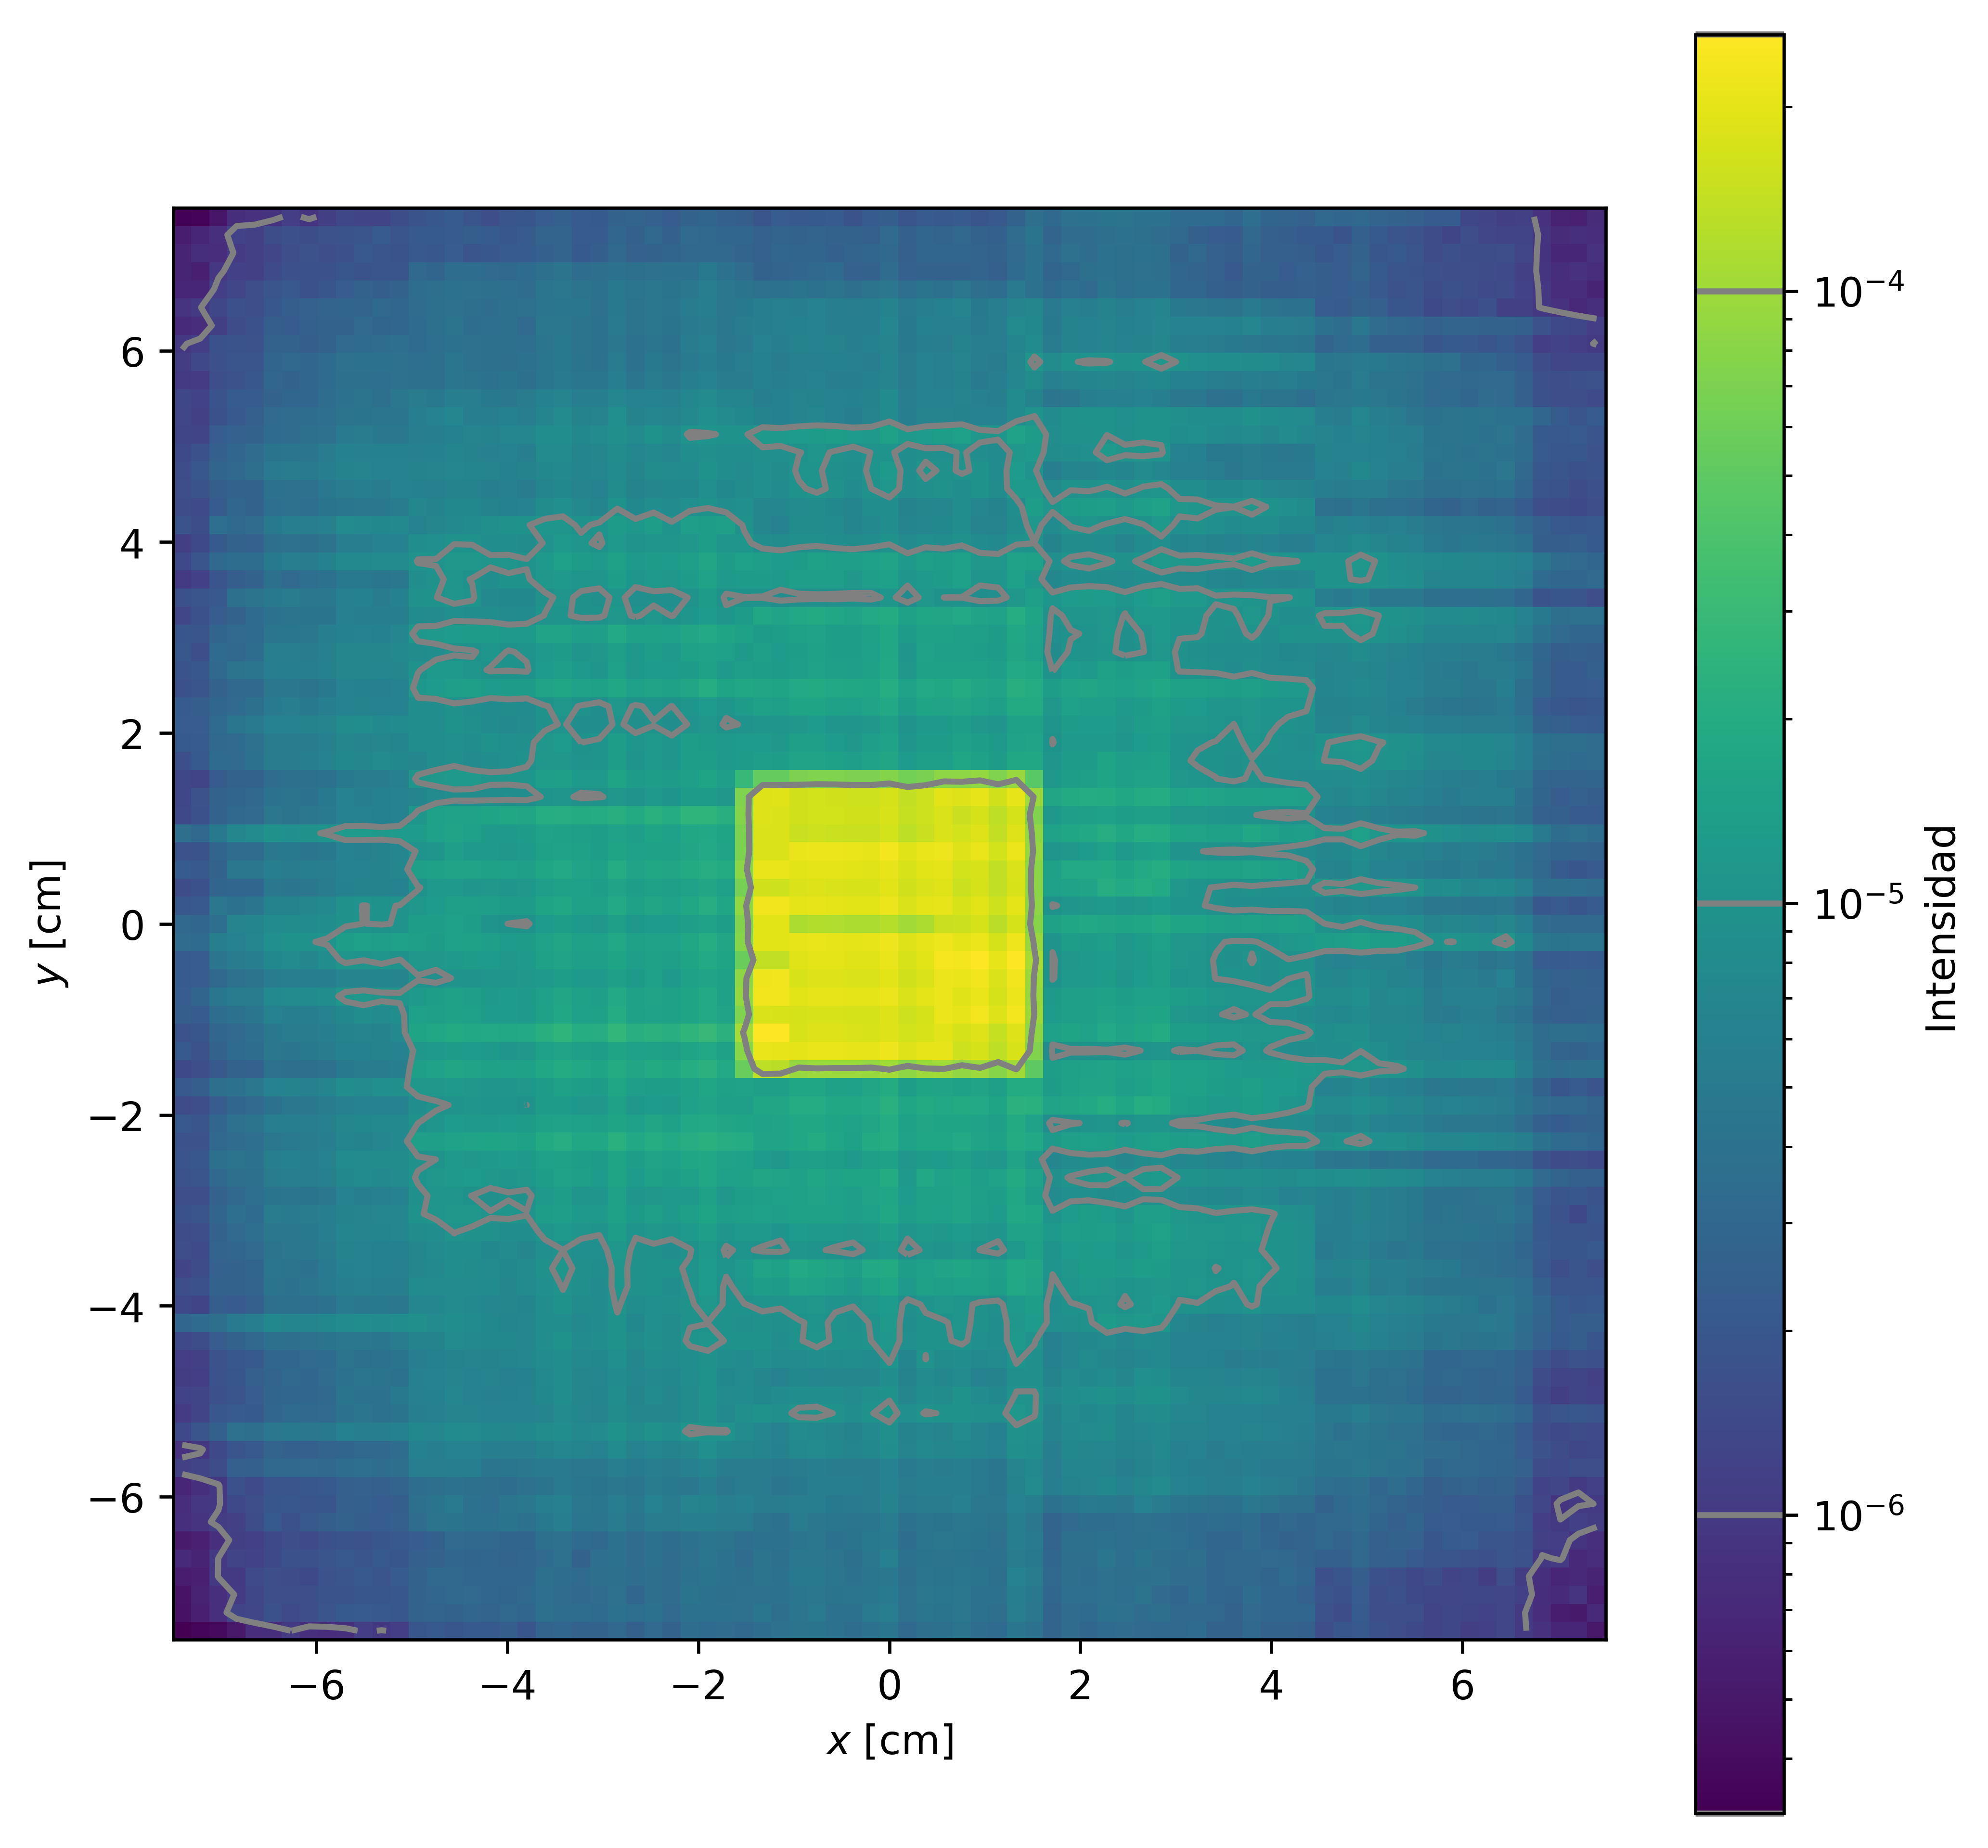
\includegraphics[width=0.6\textwidth]{xy_4.png}
    \caption{Distribución remuestreada en el plano $X$–$Y$ para el caso 4 de bineado adaptativo con bordes definidos por el usuario.}
    \label{fig:xy_4}
\end{figure}

\subsection{Análisis preliminar de los resultados}

El análisis realizado en esta sección permitió evaluar las 4 configuraciones de bineado. Se evidenció que los histogramas adaptativos ofrecen una representación más fiel del comportamiento original, incluso en ausencia de bordes manuales, en comparación con los esquemas de bineado uniforme.

Sin embargo, también se observó que la incorporación de bordes definidos por el usuario continúa siendo una herramienta útil cuando se dispone de conocimiento previo de la fuente. Estos bordes permiten guiar al algoritmo, segmentando zonas relevantes, lo que facilita a asignar mayor resolución a otras zonas del espacio de fases.

Por otro lado, se identificaron limitaciones en el esquema adaptativo. En particular, el análisis de la variable direccional $\mu$ —cuarta en el orden de las variables— evidenció un exceso de bines debido a la baja cantidad de partículas en los subconjuntos. Esta excesiva resolución produce la reproducción del ruido estadístico en lugar de su suavizado.

Para mitigar este efecto, se propone reducir progresivamente la cantidad de bines de los histogramas tanto macro como micro a medida que se avanza en el orden de segmentación. Este ajuste permitiría conservar la capacidad de detección fina en las primeras variables, mientras se evita la sobresegmentación en etapas siguientes donde la estadística es más limitada.

En la siguiente sección, se aplicará esta estrategia a modo de configuración definitiva: se volverá a procesar el archivo de partículas original empleando un esquema de segmentación jerárquica con reducción progresiva de la cantidad de bines.

\section{Procesamiento optimizado del archivo de partículas}

Con base en los resultados del procesamiento preliminar, se definió una configuración optimizada para generar la fuente distribucional. El objetivo fue preservar la fidelidad de la representación estadística, evitando al mismo tiempo la sobresegmentación de los subconjuntos que se observó en configuraciones anteriores.

Para minimizar la fragmentación del conjunto de datos, se optó por utilizar la menor cantidad posible de macrogrupos, manteniendo el orden de las variables usado previamente. La configuración seleccionada fue: 
\[
n_\text{macro} = [3, 5, 3, 3]
\]
Este esquema permitió trabajar con subconjuntos de mayor estadística en las etapas siguientes del procesamiento, mejorando así el procesamiento de los histogramas micro.

Asimismo, se eligió una cantidad reducida de microgrupos que garantizara una representación adecuada con un nivel de suavizado compatible con la estadística disponible. El esquema utilizado fue:
\[
n_\text{micro} = [30, 10, 9, 16, 4]
\]
Este conjunto es decreciente con el orden de segmentación, excepto en el caso de $\mu$, donde se incrementó el número de bines para mejorar la resolución en la zona cercana a $\mu \approx 0$.


La Figura \ref{fig:let_5} muestra la distribución remuestreada de letargía obtenida con esta configuración. Se observa una representación precisa de la delta correspondiente a la letargía mínima, así como una buena resolución en la región de termalización. En la zona intermedia, donde la densidad estadística es menor, el suavizado logrado resulta adecuado y coherente con la tendencia de la distribución original.

\begin{figure}[H]
    \centering
    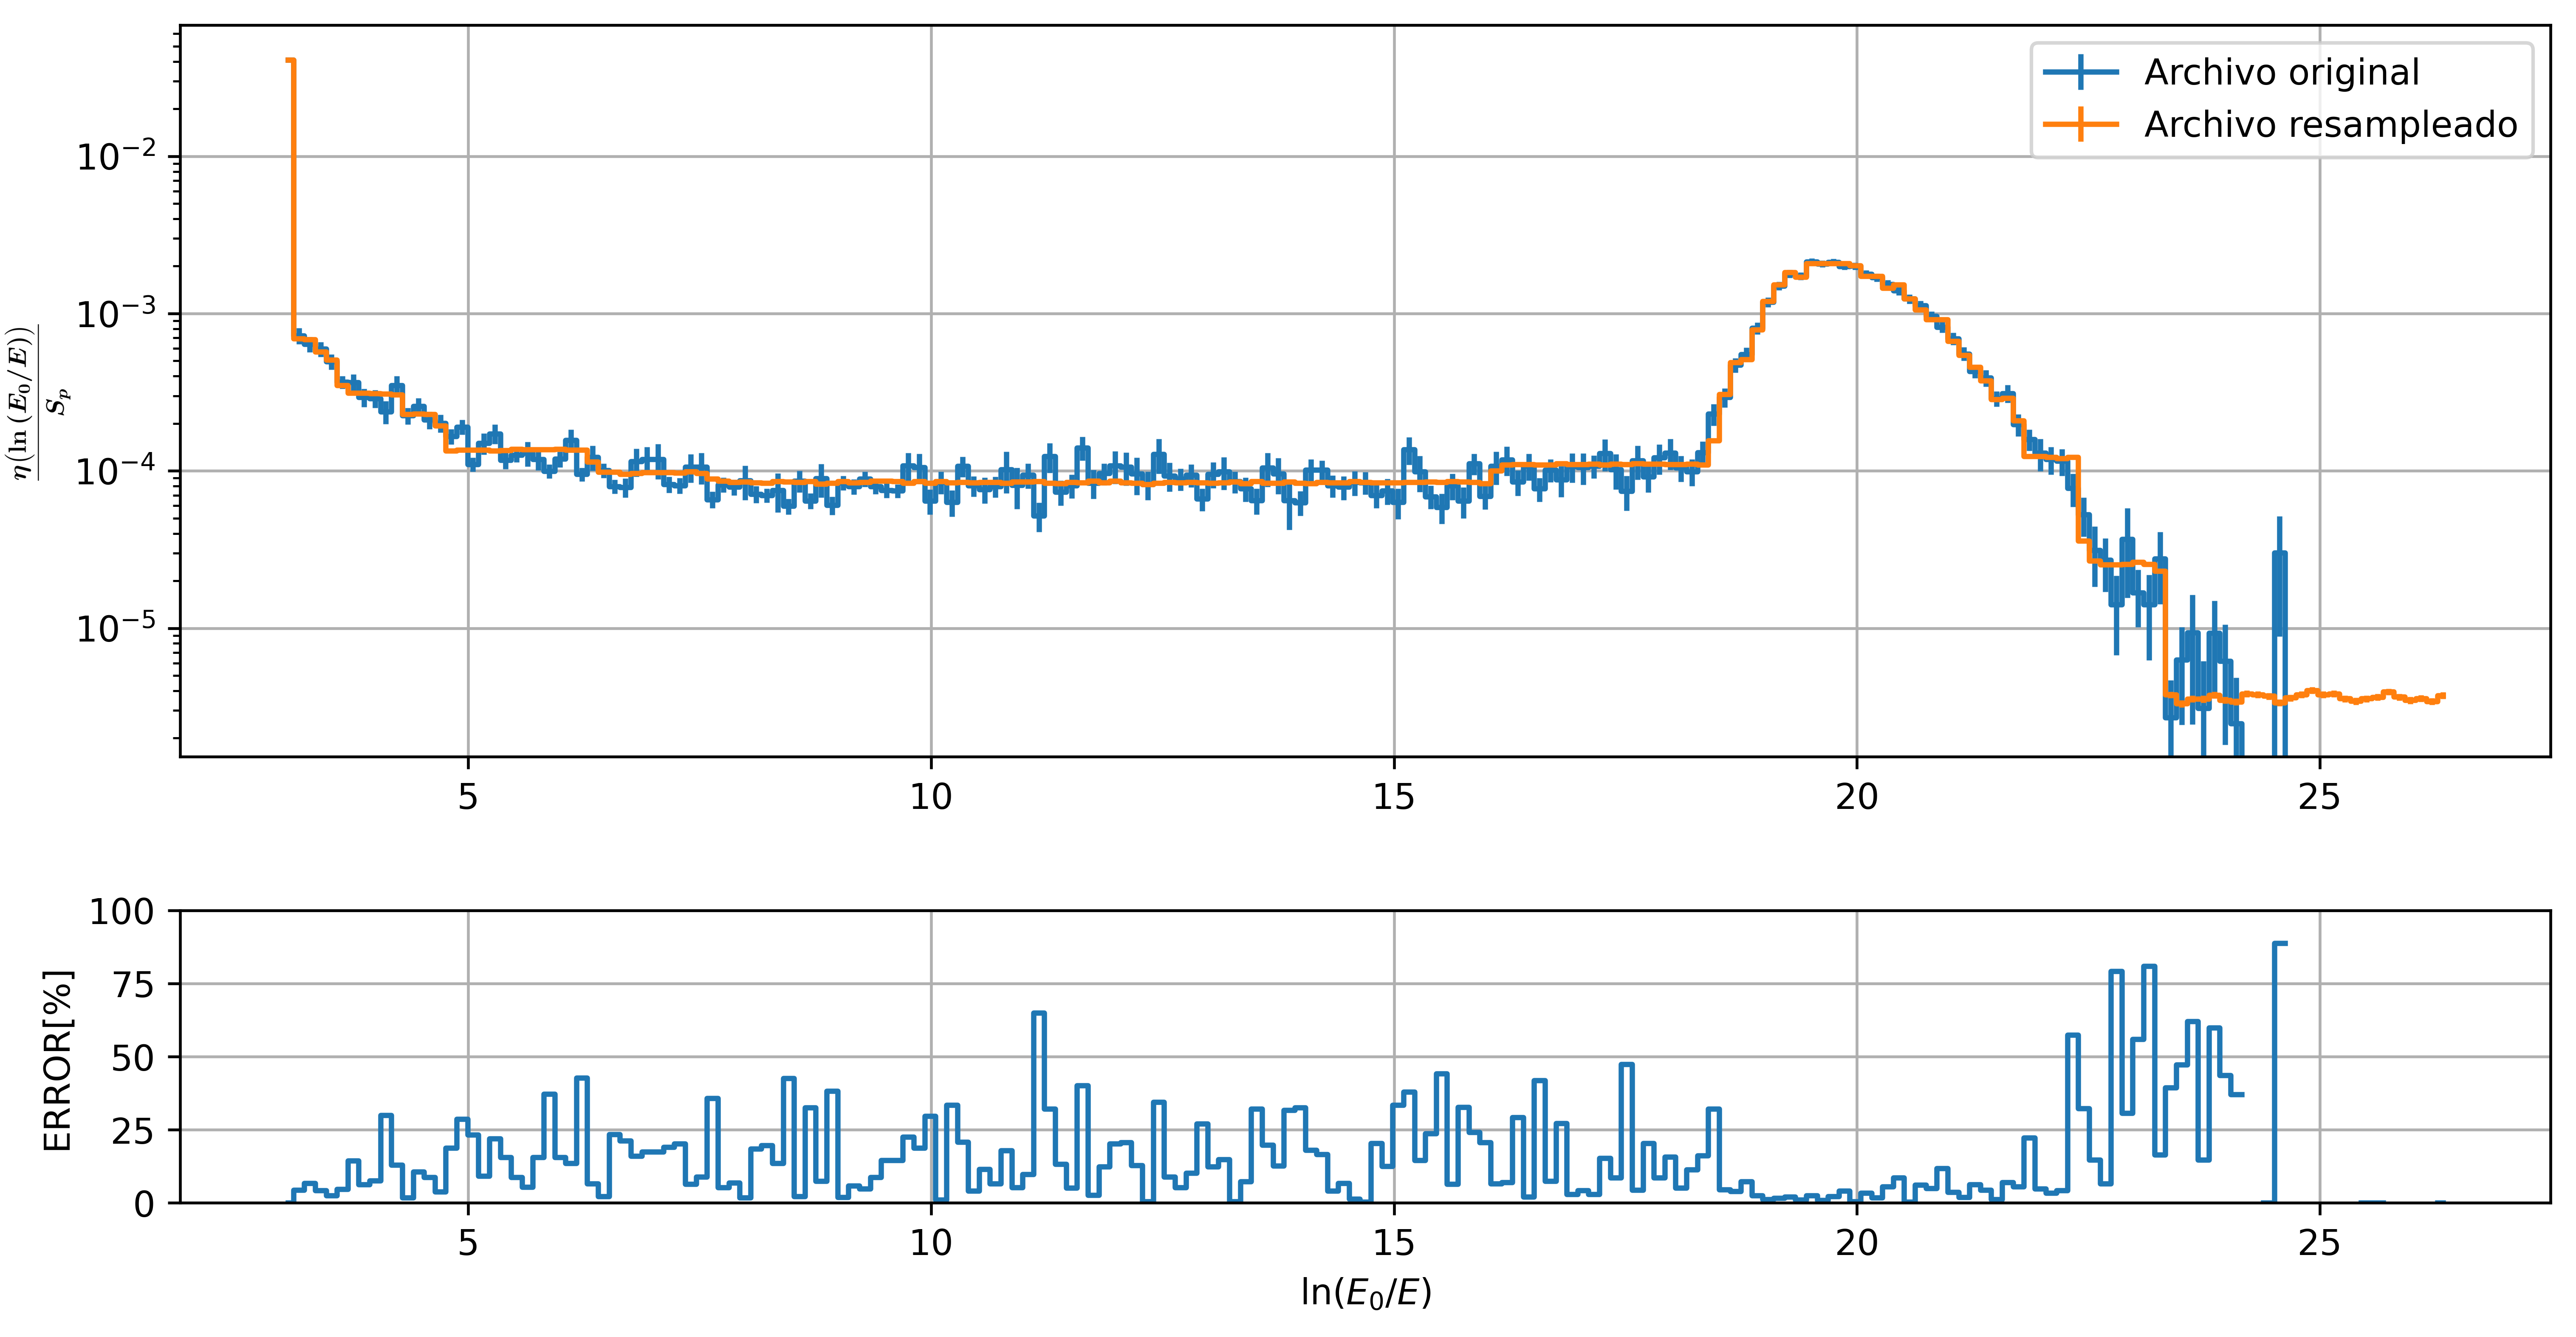
\includegraphics[width=\textwidth]{let_5.png}
    \caption{Distribución remuestreada de letargía utilizando la configuración optimizada de macro y microgrupos.}
    \label{fig:let_5}
\end{figure}

En la Figura \ref{fig:mu_5} se muestra la distribución remuestreada de $\mu$. Se obtiene una correcta representación del pico en $\mu = 1$, asociado a neutrones colimados, así como un buen seguimiento en el resto del dominio, sin evidencia de ruido estadístico excesivo.

\begin{figure}[H]
    \centering
    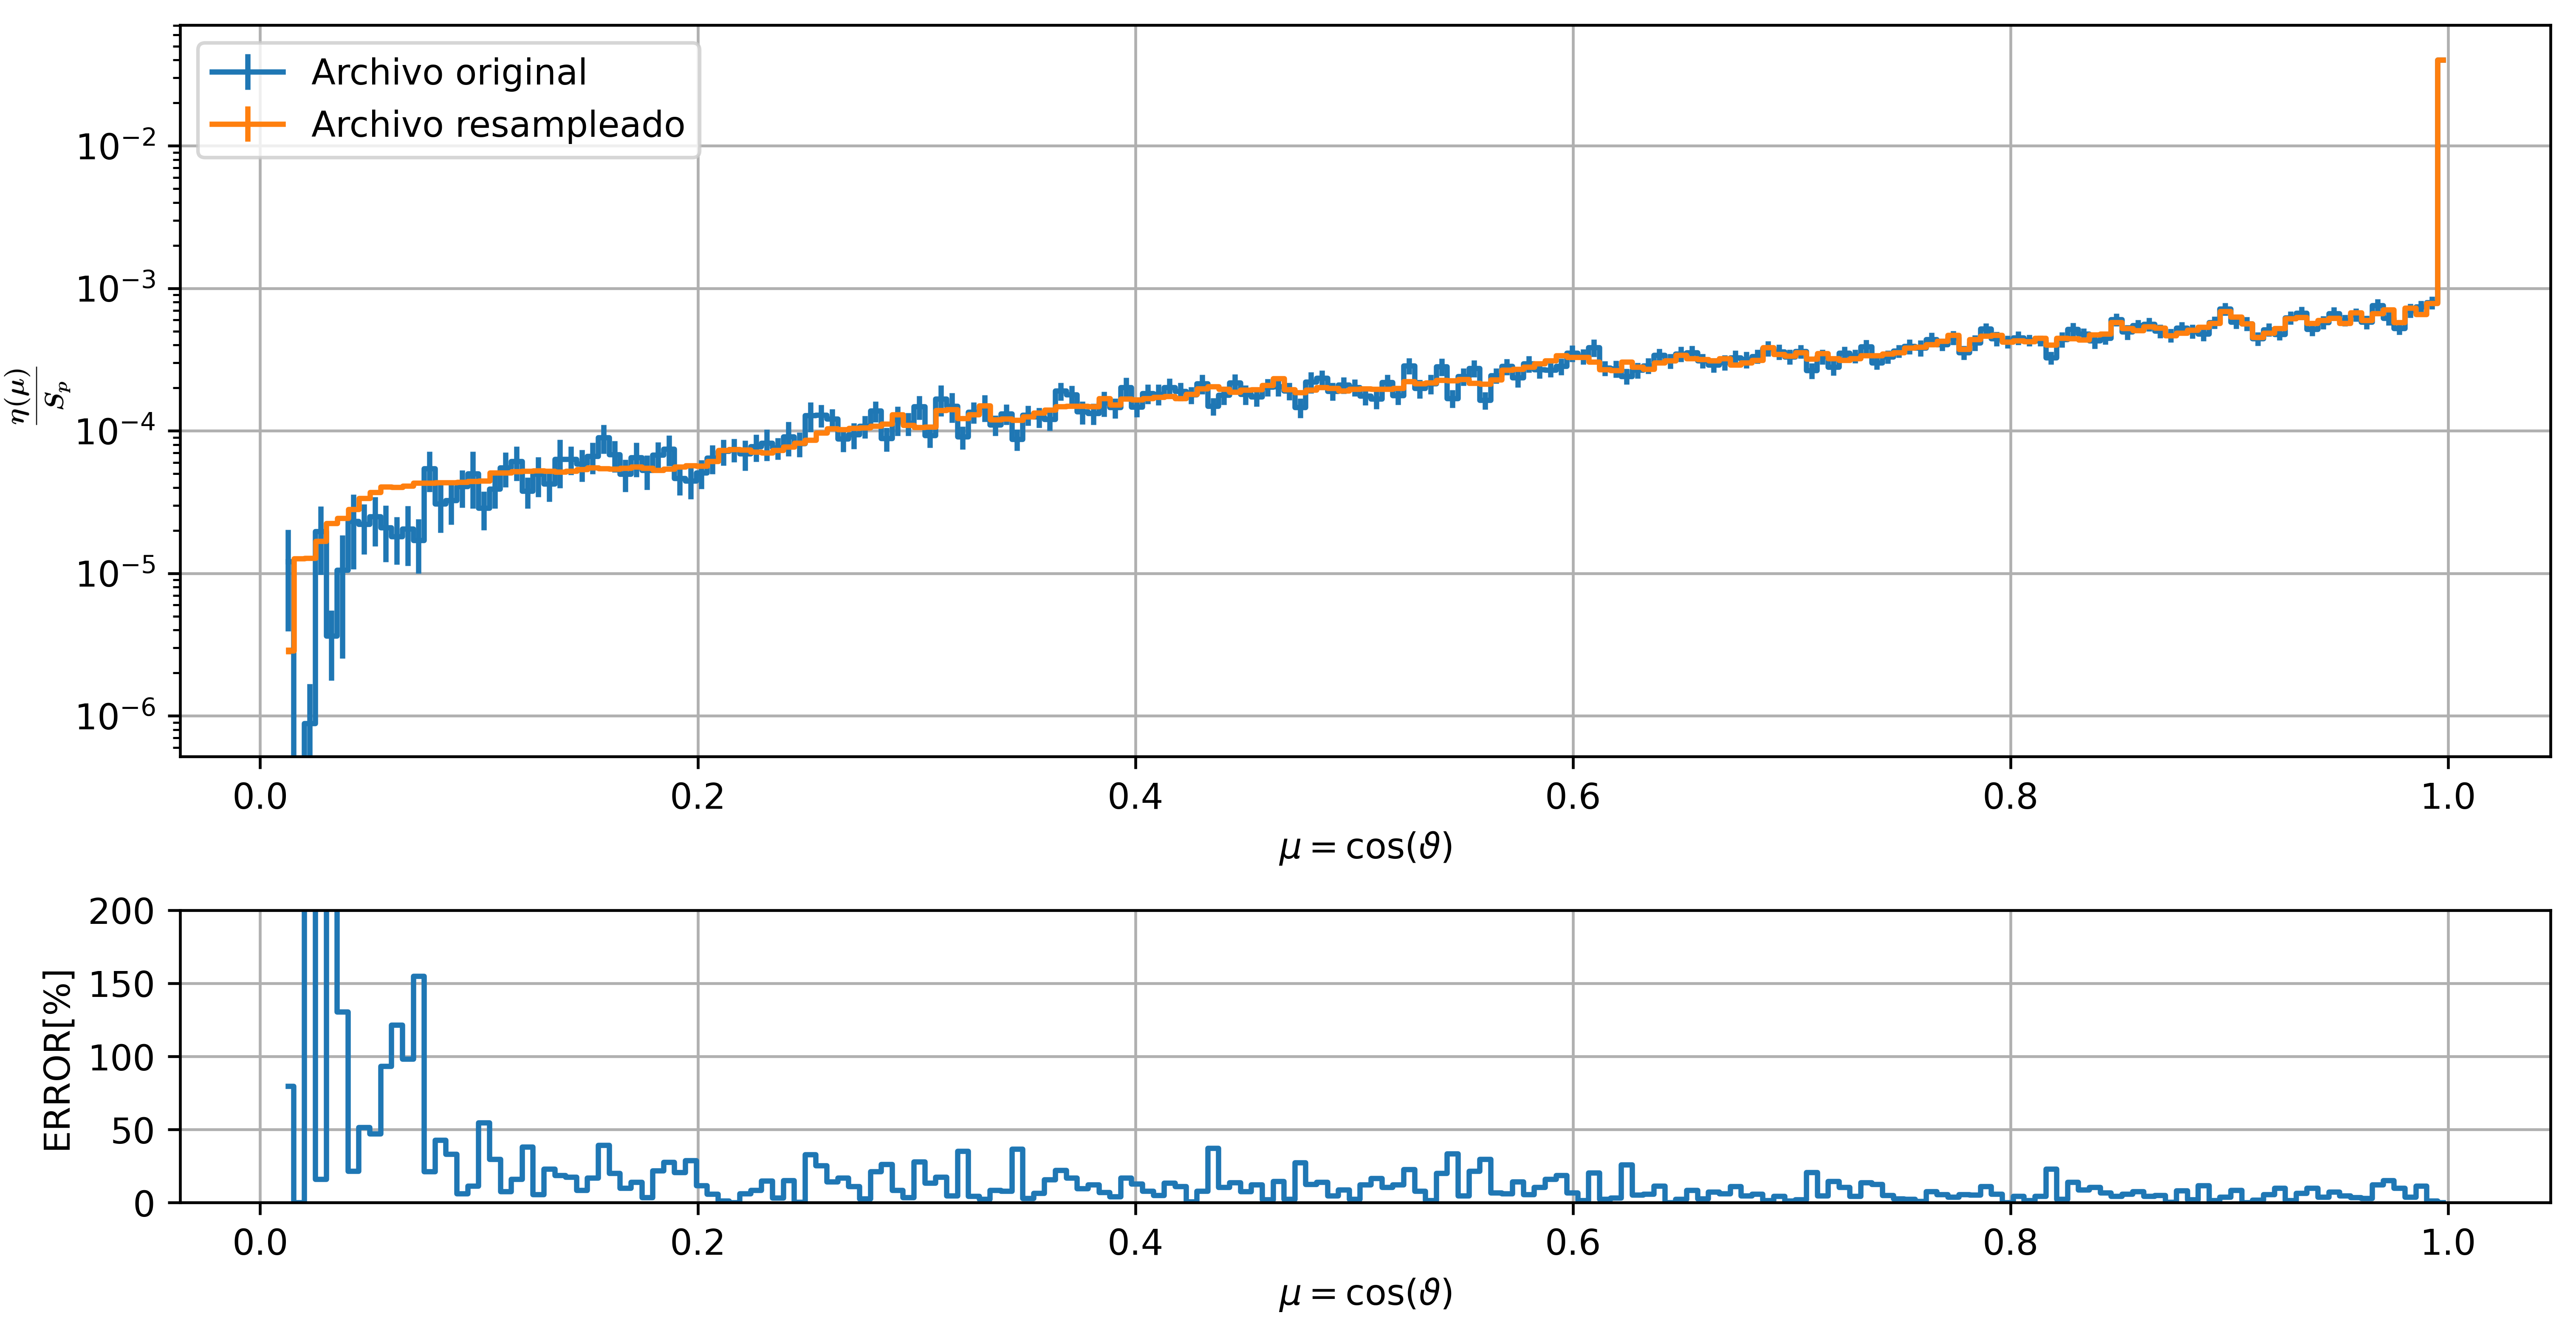
\includegraphics[width=\textwidth]{mu_5.png}
    \caption{Distribución remuestreada de $\mu$ utilizando la configuración optimizada.}
    \label{fig:mu_5}
\end{figure}

La Figura \ref{fig:xy_5} presenta la distribución espacial en el plano $X$-$Y$. Se observa una representación precisa del canal de vacío, sin generación espuria de partículas en el agua. Sin embargo, la resolución en la región del agua es inferior a la alcanzada en configuraciones con mayor cantidad de macrogrupos. Este efecto refleja el compromiso asumido: evitar segmentar en exceso regiones con baja estadística para preservar la calidad aguas abajo.

\begin{figure}[H]
    \centering
    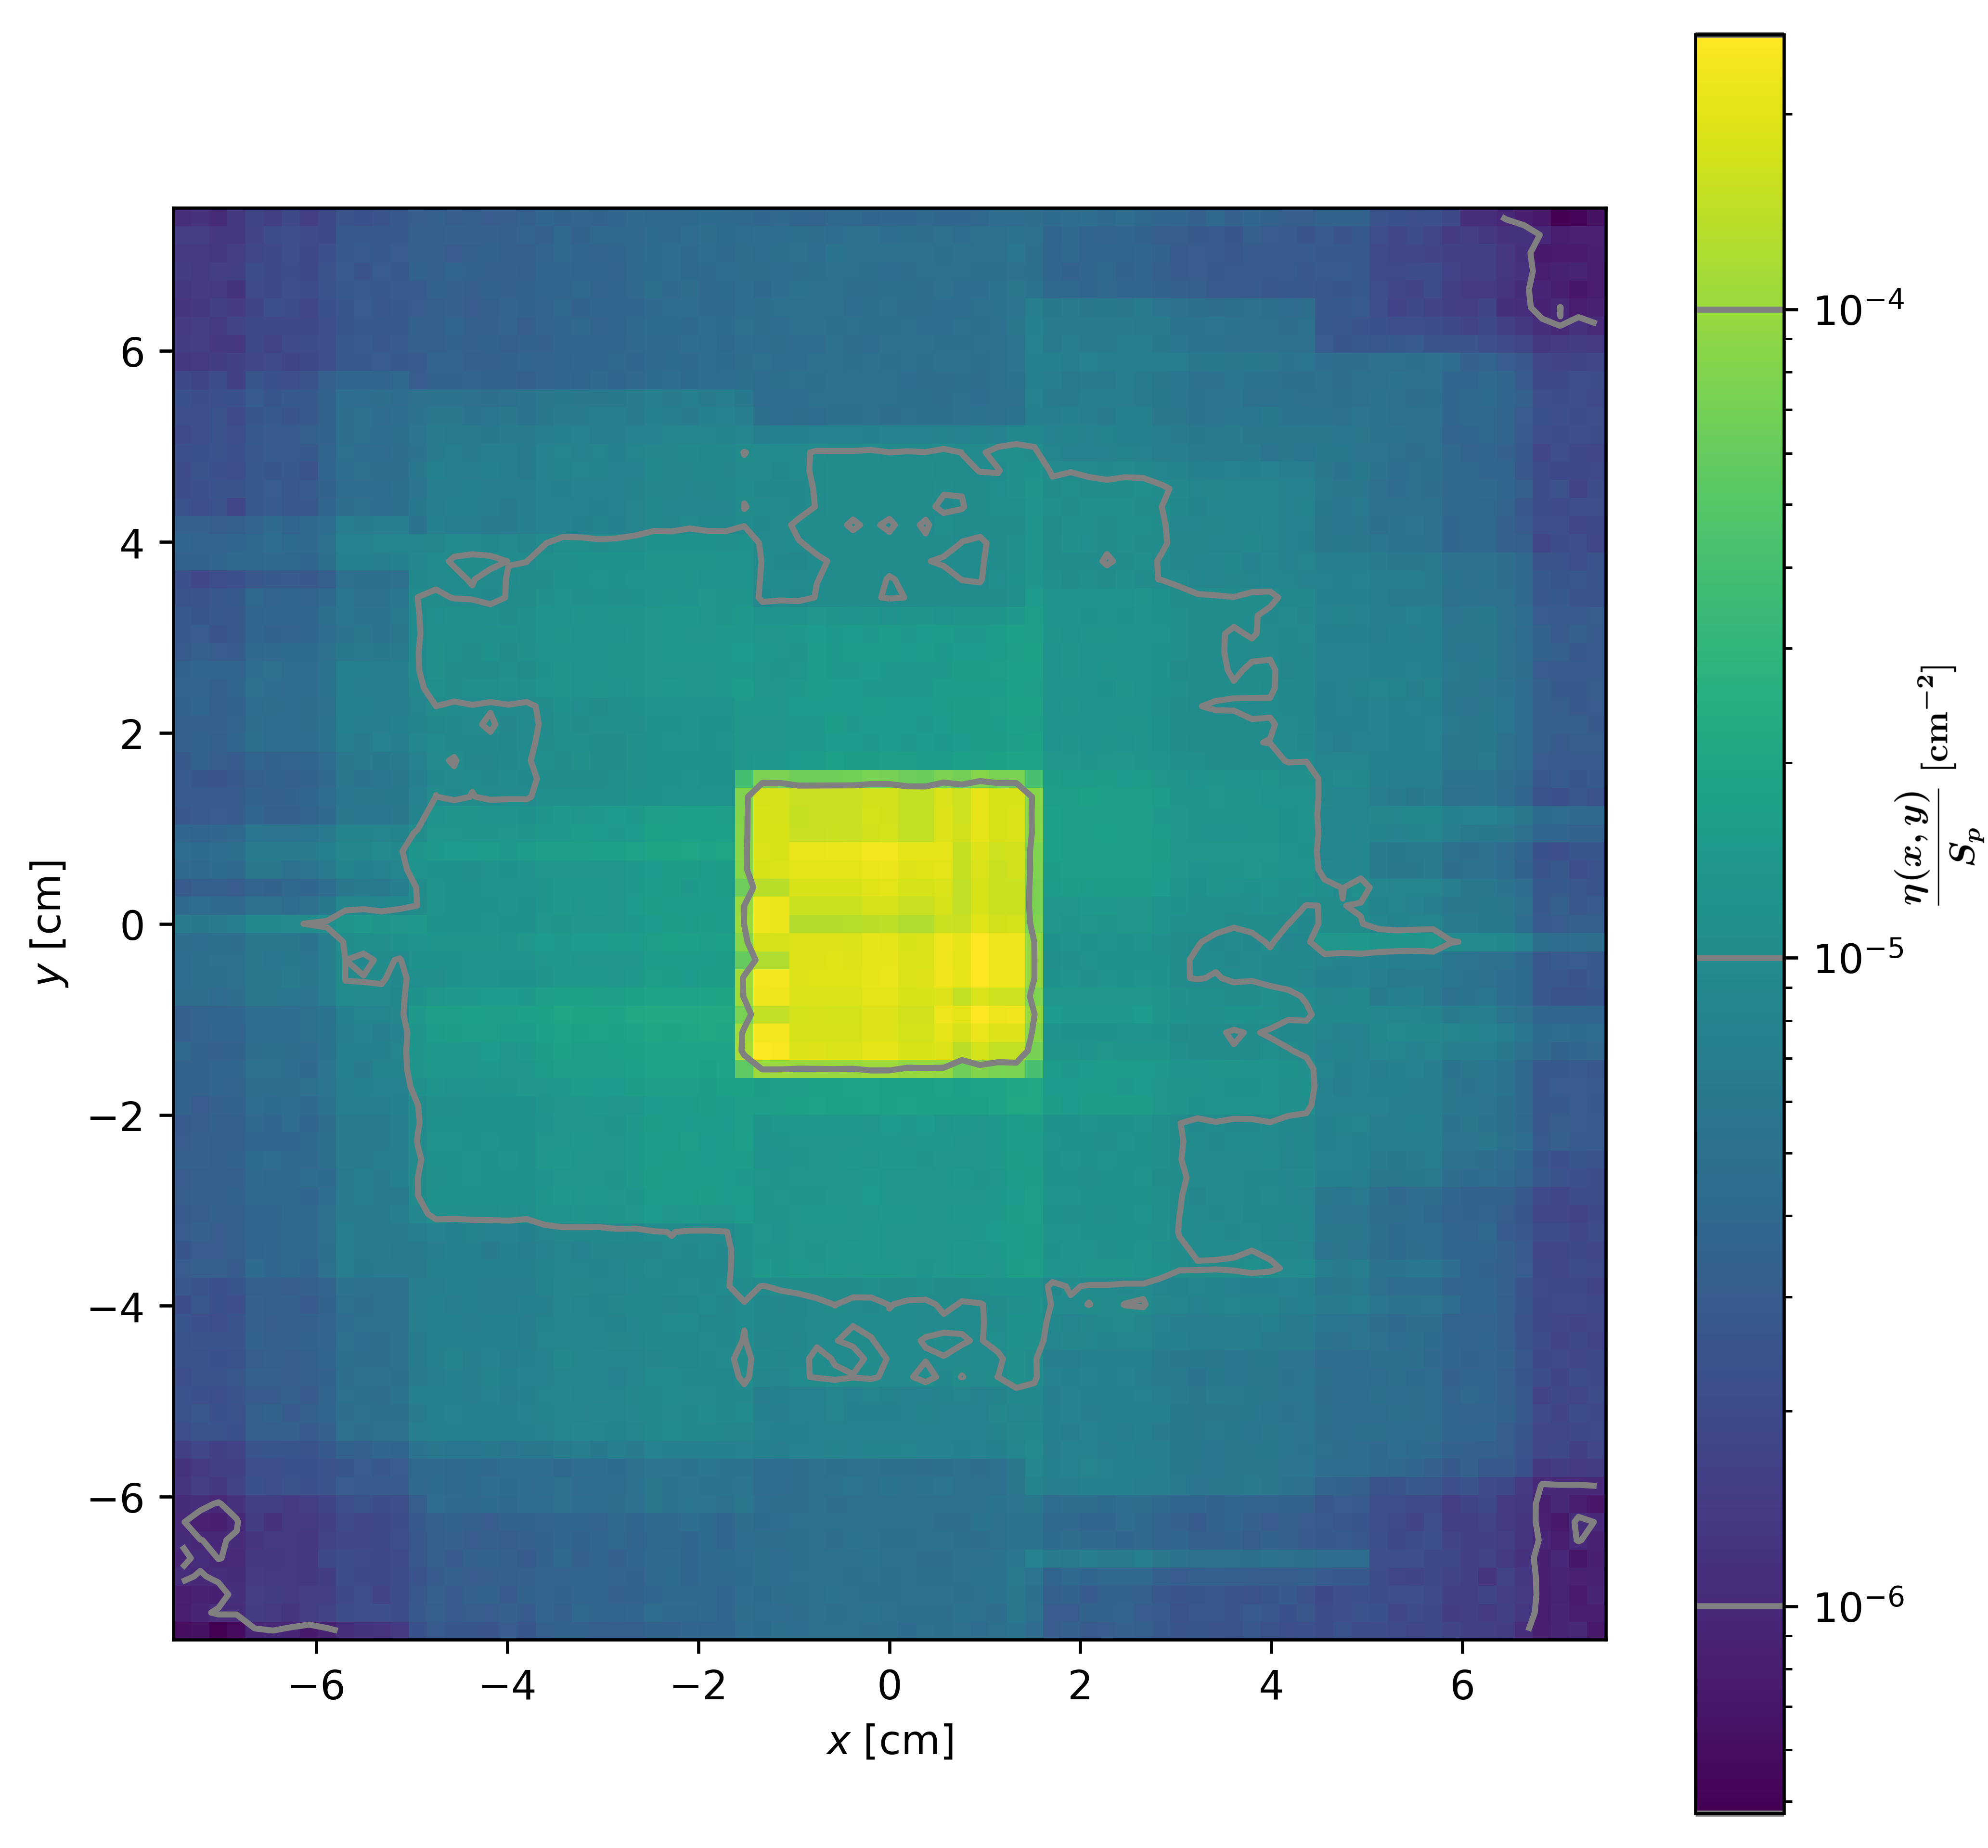
\includegraphics[width=0.6\textwidth]{xy_5.png}
    \caption{Distribución remuestreada en el plano $X$-$Y$ con configuración final optimizada.}
    \label{fig:xy_5}
\end{figure}


La configuración descrita será utilizada como base para realizar la simulación definitiva desde la superficie de acople en adelante. En la próxima sección se presentan los resultados obtenidos y se comparan contra la simulación original de referencia, ejecutada con una mayor cantidad de partículas.

\section{Resultados de la simulación comparativa}

Para validar los resultados se evaluaron distintas magnitudes físicas a lo largo del eje del sistema:

\begin{itemize}
    \item Flujo escalar a lo largo del tubo: en agua, y en vacío.
    \item Espectro energético sobre una superficie a $z = 80\,\text{cm}$.
    \item Corriente sobre una superficie a $z = 80\,\text{cm}$.
\end{itemize}

A su vez se aplicó el metodo de reducción de varianza de ventanas de peso implementado en \texttt{OpenMC} para mejorar la estadística en el agua.

\subsection{Comparación del perfil de flujo a lo largo del canal}

Con el objetivo de validar la fuente distribucional generada, se realizó una simulación de referencia desde el inicio del conducto, utilizando una cantidad elevada de partículas para asegurar una buena convergencia estadística, según se muestra en la Figura~\ref{fig:esquema_remuestreo}. A partir de esta simulación se obtuvo el perfil de flujo original a lo largo del canal.

Posteriormente, se utilizó la fuente distribucional construida en la sección anterior y se ejecutó una nueva simulación iniciando desde la superficie ubicada a $z = 15$cm. Esta corrida fue llevada adelante hasta alcanzar también una buena convergencia, permitiendo así una comparación directa entre ambos resultados.

La Figura \ref{fig:flujo_comparacion} muestra los perfiles de flujo escalar obtenidos en ambas regiones del conducto: la región de agua moderadora (\ref{fig:flujo_agua}) y el canal de vacío (\ref{fig:flujo_vacio}), junto con el error relativo porcentual.

\begin{figure}[H]
    \centering
    \begin{subfigure}[t]{0.48\textwidth}
        \centering
        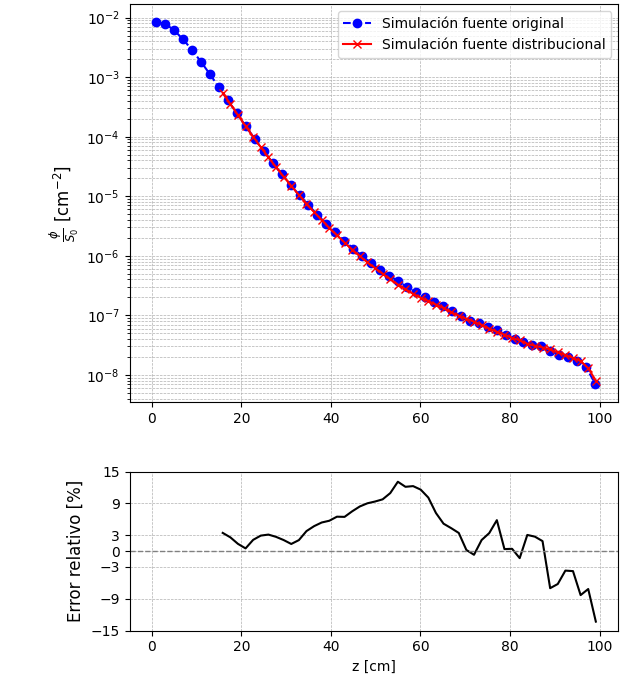
\includegraphics[width=\textwidth]{flujo_agua.png}
        \caption{Región de agua.}
        \label{fig:flujo_agua}
    \end{subfigure}
    \hfill
    \begin{subfigure}[t]{0.48\textwidth}
        \centering
        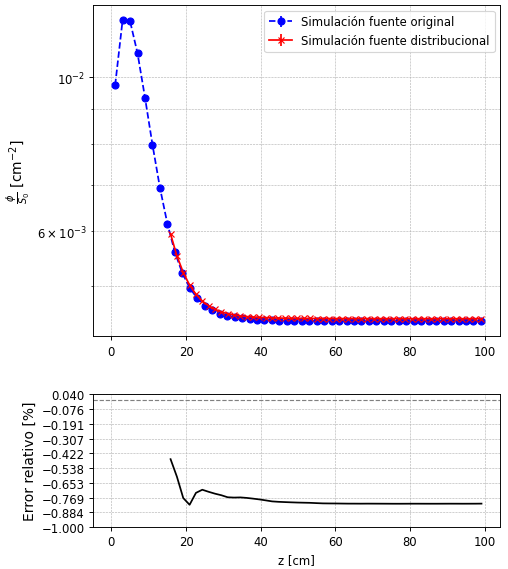
\includegraphics[width=\textwidth]{flujo_vacio.png}
        \caption{Canal de vacío.}
        \label{fig:flujo_vacio}
    \end{subfigure}
    \caption{Comparación entre los perfiles de flujo escalar obtenidos mediante la fuente original (simulación larga desde el inicio del conducto) y mediante la fuente distribucional (simulación desde la superficie intermedia). En ambas regiones se muestra también el error relativo porcentual.}
    \label{fig:flujo_comparacion}
\end{figure}
% \begin{figure}[H]
%     \centering
%     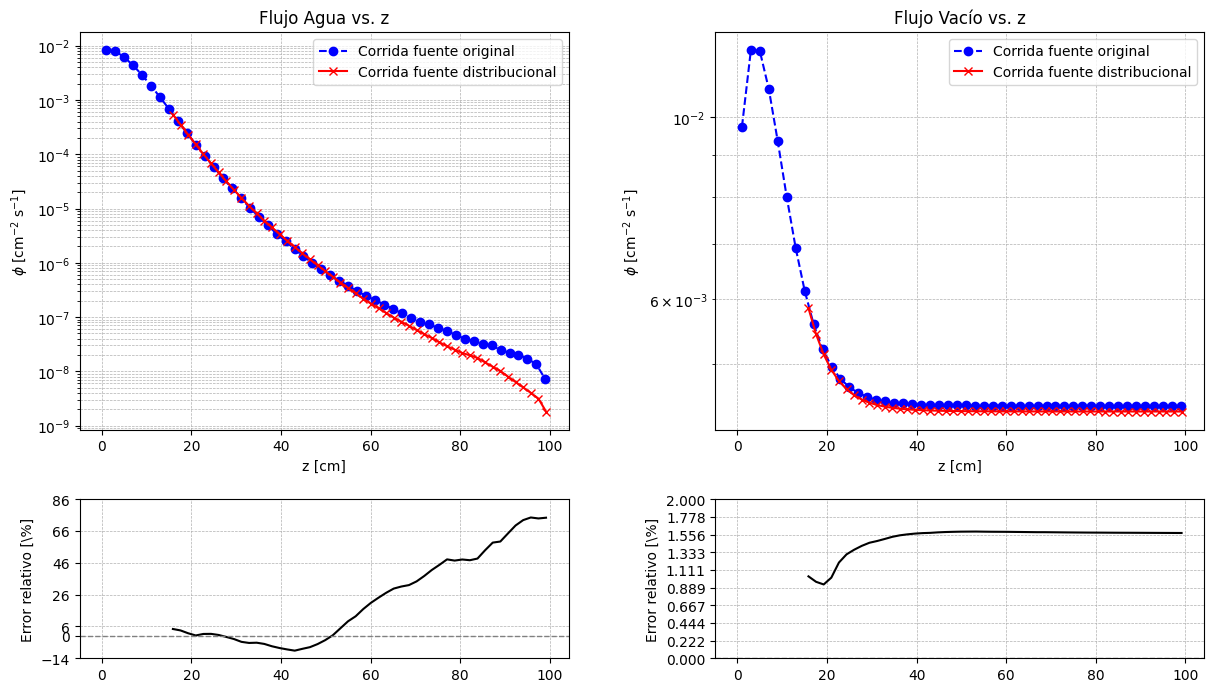
\includegraphics[width=\textwidth]{flujo_1.png}
%     \caption{Comparación entre los perfiles de flujo escalar obtenidos mediante la fuente original (simulación larga desde el inicio del conducto) y mediante la fuente distribucional (simulación desde la superficie intermedia). A la izquierda: región de agua; a la derecha: canal de vacío. En ambos casos se muestra el error relativo.}
%     \label{fig:flujo_comparacion}
% \end{figure}

En la región de agua (Figura \ref{fig:flujo_agua}), se observa un error relativo que no converge con la distancia al origen de la fuente. Este comportamiento se explica por la escasa densidad de peso estadístico presente originalmente en esta región del archivo de partículas original (ver Tabla~\ref{tab:particulas_pesos}), lo cual dificultó la reconstrucción adecuada de su distribución.

En cambio, en el canal de vacío (Figura \ref{fig:flujo_vacio}), se logra una reconstrucción de mayor precisión del perfil original. El error relativo se mantiene por debajo del 1\% en todo el tramo analizado, lo que indica una adecuada correspondencia entre la fuente generada y el perfil de referencia. Cabe destacar que parte del error observado se debe a diferencias entre las distribuciones de corriente presentes en el archivo de partículas original —limitado en estadística— y la simulación larga de referencia. No obstante, las formas del perfil en ambas simulaciones muestran concordancia, validando el enfoque implementado.

\subsection{Comparación del espectro en la salida del canal}

Además del perfil de flujo, se analizó el espectro registrado en la superficie ubicada a $z = 80$~cm. En ambas simulaciones —la original desde el inicio del conducto y la simulación utilizando la fuente distribucional— se registró el espectro de neutrones incidentes sobre dicha superficie. La Figura \ref{fig:espectro_comparacion} muestra los espectros normalizados por neutrón de fuente obtenidos para ambas simulaciones. 

En la Figura \ref{fig:espectro_agua}, correspondiente a la región de agua, se observa que el espectro generado por la fuente distribucional presenta una buena aproximación en las regiones de alta letargía, donde se encuentran los neutrones termalizados. El error relativo en esa zona es bajo, lo que indica que la fuente remuestreada logró capturar adecuadamente la estructura del espectro original.

En la Figura \ref{fig:espectro_vacio} se observa una correcta aproximación en la región de letargía correspondiente a $E = 1~MeV$, donde el error relativo es muy bajo. Esto indica que el remuestreo de los neutrones colimados que se propagan por el canal de vacío se realizó correctamente. Este resultado está en concordancia con lo observado previamente en el perfil de flujo en dicha región (ver Figura \ref{fig:flujo_vacio}), donde el error se mantuvo por debajo del 1\%. En cambio para regiones de mayor letargía, correspondientes a neutrones que han colisionado y se propagan por la región de vacío, se observa un error relativo mayor. 

\begin{figure}[H]
    \centering
    \begin{subfigure}[t]{0.48\textwidth}
        \centering
        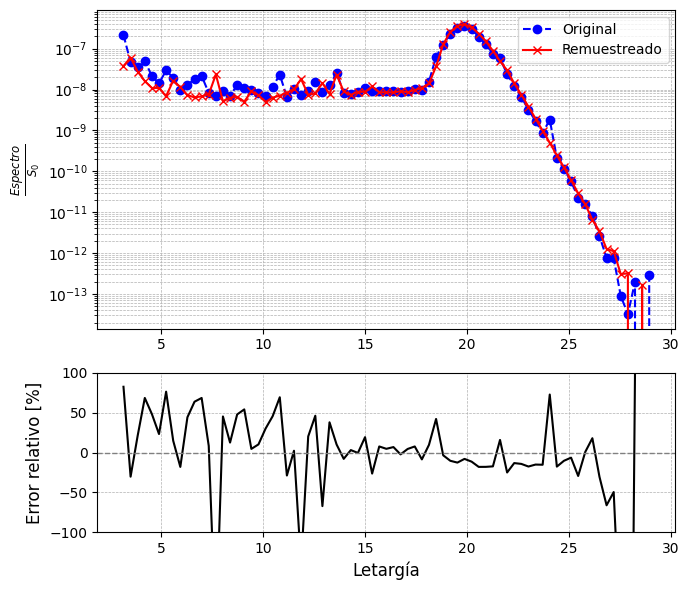
\includegraphics[width=\textwidth]{espectro_agua.png}
        \caption{Región de agua.}
        \label{fig:espectro_agua}
    \end{subfigure}
    \hfill
    \begin{subfigure}[t]{0.48\textwidth}
        \centering
        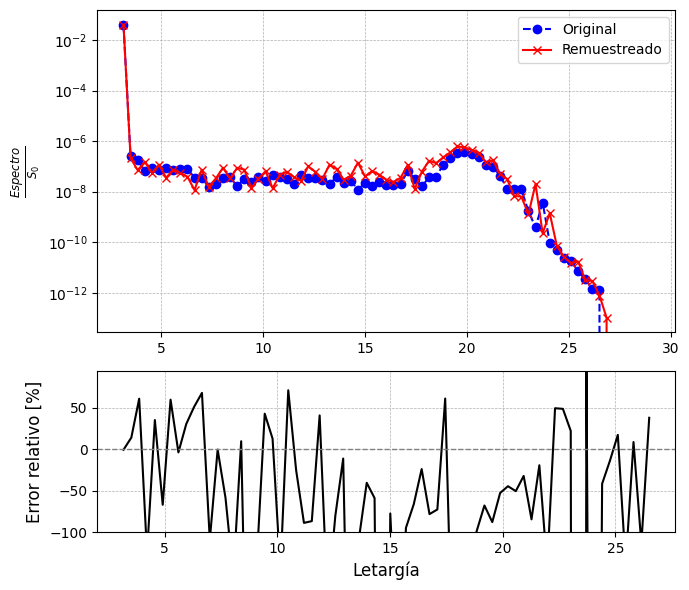
\includegraphics[width=\textwidth]{espectro_vacio.png}
        \caption{Canal de vacío.}
        \label{fig:espectro_vacio}
    \end{subfigure}
    \caption{Comparación del espectro de neutrones en la superficie a $z = 80$~cm para las simulaciones original y remuestreada. En ambos casos se incluye también el error relativo porcentual.}
    \label{fig:espectro_comparacion}
\end{figure}


% En cambio, para regiones de mayor letargía, correspondientes a neutrones presentes en el agua, se observa una subestimación en el espectro generado por la fuente distribucional. Este efecto se explica por la baja estadística disponible originalmente en el agua, lo que dificultó capturar adecuadamente dicha contribución. Tal como se mencionó en la sección anterior, el perfil de flujo en la región de agua mostró una atenuación progresiva con la distancia (ver Figura \ref{fig:flujo_comparacion}, izquierda), fenómeno que se reproduce aquí en forma espectral.

% A pesar de esta diferencia en magnitud, se destaca que la forma general del espectro se mantiene coherente entre ambas simulaciones. Esto sugiere que, si bien el contenido total en la región del agua fue subrepresentado, el método logró capturar correctamente la estructura cualitativa del espectro original.

\subsection{Comparación de la corriente}

Se analizó la corriente total de neutrones atravesando la superficie ubicada a $z = 80$~cm para ambas simulaciones. En la simulación original, ejecutada desde el inicio del canal con alta estadística, se obtuvo una corriente normalizada de
\[
J_{\text{original}} = (4.005 \pm 0.003) \times 10^{-2} \; \text{neutrones por neutrón fuente}.
\]

Por otro lado, la simulación realizada con la fuente remuestreada arrojó un valor de
\[
J_{\text{remuestreada}} = (4.037 \pm 0.008) \times 10^{-2} \; \text{neutrones por neutrón fuente}.
\]

Esto representa un 100.8\% del valor original, lo cual indica una aceptable conservación de la corriente total. 


\section{Conclusiones preliminares}

El estudio aplicado al caso de un canal de vacío rodeado por agua permitió evaluar el desempeño del método de generación de fuentes distribucionales basado en histogramas multidimensionales. Este caso representa una situación física relevante y sensible, ya que involucra la coexistencia de poblaciones de neutrones con comportamientos distintos: una colimada y monoenergética en el vacío, y otra dispersa y moderada en el agua.

Los principales resultados obtenidos son:

\begin{itemize}
    \item Se logró reconstruir el flujo escalar y el espectro en el canal de vacío. La región colimada de neutrones sin colisiones fue correctamente representada por el método propuesto.
    
    % \item La reconstrucción del flujo y el espectro en el agua presentó limitaciones más marcadas, debidas a la poca estadistica en el agua en el archivo de particulas original.

    \item Se observó que el uso de histogramas adaptativos permite una representación más equilibrada y autónoma del espacio de fases, sin necesidad de intervención manual. No obstante, la incorporación de bordes definidos por el usuario sigue siendo una herramienta útil cuando se dispone de información a priori sobre el sistema, especialmente para evitar mezclas artificiales entre poblaciones diferenciadas.

    \item La implementación de una reducción progresiva en la resolución de los histogramas macro y micro resultó eficaz para evitar el sobreajuste en conjuntos de poca estadística, evitando amplificar el ruido estadístico.
\end{itemize}

% Sin embargo, es importante destacar que la calidad de la fuente generada depende de la calidad estadística del archivo de partículas original. Este punto se discute en mayor profundidad en el Apéndice \ref{app:B}, donde se analiza el mismo caso utilizando un archivo de partículas con mayor estadística. En dicho análisis se obtienen mejoras significativas en la reconstrucción de la región de agua.


